%! Author = sriadityavedantam
%! Date = 3/25/26

\part{Real Analysis}

\chapter{Introduction}
\epigraph{AI is like how a chocolate croissant is... Irresistible}{\textit{Joseph H.G Fu}}

\epigraph{The natural numbers are the work of God.}{\textit{Leopold Kronecker}}

\epigraph{Sets are like machine code, its one of the ways you can have it, but you will never catch me talking about categories.}{\textit{Joseph H.G Fu}}

\epigraph{You can't get anywhere in life without desire.}{\textit{Joseph H.G Fu}}

\newpage

\epigraph{Do not have a belabored proof. If you are able to convince yourself and show you understand what is happening, then there is nothing more that is needed. Many undergraduates write too much that it makes me less convinced.}{\textit{Joseph H.G Fu}}

\newpage
\begin{itemize}
    \item First part: Undergraduate Studies. We follow Abbott Chapter 1-7.
    \item We follow Abbott `Understanding Analysis':
    \begin{itemize}
        \item Chap 1 `The Real Numbers'
        \item Chap 2 `Sequences and Series'
        \item Chap 3 `Basic Topology of $\r$'
        \item Chap 4 `Functional Limits and Continuity'
        \item Chap 5 `The Derivative'
        \item Chap 6 `Sequences and Series of Functions'
        \item Chap 7 `The Riemann Integral'
    \end{itemize}
    \item Second part: Semi-Graduate Studies. We follow Abbott Chapter 8 only.
    \item 20 graduate problems (solve them during the semester) No feedback during the semester, but asking questions is allowed. Working together is allowed.
    \item Exam (1 paged cheat-sheet, closed book, fresh dissimilar questions)
\end{itemize}

\chapter{The Real Numbers}

%! Author = sriadityavedantam
%! Date = 3/25/26

\section{Some Preliminaries}

\lesson{1}{Wednesday 13 August 2025 09:10}{Day 1}

Though things arise naturally out of studies like Algebra, some claim that we need to go beyond
such, and apply some intuition and \('\)analytical\('\) prowess to find ideas from what may seem
abstract or uncorrelated.
Real Analysis gave foundation and birth to many different fields we
know today, including most of the applied math workforce, such as Chemists, Physicists,
Biologists, Meteorologists, and so forth.
But within math, also optimization, complex analysis,
differential equations, differential geometry, and so forth.
It is essentially a cornerstone of
mathematics, regarded by many.

\begin{definition}[Real Numbers]
	\textbf{The complete ordered} field that contains $\q$.
\end{definition}

\begin{definition}[Rational Numbers]
    \[\q = \{\dfrac{a}{b} : a,b\in\z, b\neq 0\}\]
\end{definition}

\begin{definition}[Integers]
	\[\z = \{\pm n : n\in\n\}\cup\{0\}\]
\end{definition}

\begin{definition}[Naturals]
	\[\n = \{1,2,\ldots\}\]
\end{definition}

\begin{example}[Another Defintion of Rationals]
    It can be said that the rationals can be defined like the following.
	\[\q = \z\times (\z\setminus\{0\})\]
\end{example}

\begin{remark}
    Note that when were asserting $\q$, then we were unable to use the defining operator : $\coloneqq$.
\end{remark}

\begin{corollary}{
    Suppose we have $(a,b), (\alpha,\beta)\in\z\times(\z\setminus\{0\})$. Then $(a,b)\sim(\alpha,\beta)$ if and only if $\alpha b = a\beta$.
}
\end{corollary}

\begin{definition}[Equivalence Relation]
    Equivalence relations have three properties.
    Reflexivity, Symmetry, and Transitivity.
	The reflexive property holds $(a,b)\sim(a,b)$ is true.
	The symmetric property holds if $(a,b)\sim(\alpha,\beta)$, then $(\alpha,\beta)\sim(a,b)$.
	The transitive property holds if $(a,b)\sim(\alpha, \beta)$ and $(\alpha,\beta)\sim(c,d)$, then $(a,b)\sim(c,d)$.
	Prove this property for Exercise 1.
\end{definition}

\begin{remark}
Hence, we can define the rationals as the following.
	\[\q \coloneqq \dfrac{\z\times(\z\setminus\{0\})}{\sim}\]
\end{remark}

\begin{definition}[Equivalence Class]
	\[[(a,b)] + [(\alpha,\beta)] = [(a\beta + \alpha b, b\beta)]\].
\end{definition}

\begin{proposition*}[Addition is well-defined.]{
	Given $(a,b)\sim(c,d)$ and $(\alpha,\beta)\sim(\gamma,\delta)$, then $(a \beta + \alpha b, b\beta)\sim(c \delta + \beta d, d\delta)$. Prove this for Exercise 2.
}
\end{proposition*}

\begin{lemma}[Irrationality Proof]{
	There is no $q\in\q$ such that $q^2 = 2$. We call this, $\sqrt{2}$ irrational.
}
	Suppose for the sake of contradiction, if $q = \dfrac{a}{b}$ $a,b\in\z$ and $a,b$ coprime, then $q^2 = \dfrac{a^2}{b^2} = 2$.
	Thus $a^2 = 2b^2$, then $a^2$ is even.
	Furthermore, $a = 2k$ for some $k\in\z$, therefore $a^2 = 4k^2$.
	Hence, $b^2$ is even, which contradicts our coprime assumption.
\end{lemma}

\begin{remark}
	The direct statement of this lemma is:
	\begin{displayquote}
		If $q^2 = 2$, then $q\notin\q$.
	\end{displayquote}
	A contrapositive of this lemma is:
	\begin{displayquote}
		If $q\in\q$, then $q^2\neq 2$.
	\end{displayquote}
\end{remark}
%! Author = sriadityavedantam
%! Date = 3/25/26

\section{Axiom of Completness}

\lesson{2}{Friday 15 August 2025 9:10}{Day 2}

\begin{definition}[Ordering Property]
	Given $a,b\in\r$, either
	\begin{align*}
		a &> b\\
		a &= b\\
		a &< b.
	\end{align*}
\end{definition}

\begin{remark}
	Field $\r$ is complete, which means it has the least upper bound (l.u.b) property.
\end{remark}

\begin{definition}[l.u.b Property]
	If $S\subset\r$ and $S$ is bounded above, i.e.\ there is a $C\in\r$ such that $C\geq x$ for all $x\in S$, then there is some $\alpha\in\r$ which is the least upper bound for $S$.
	This means $\alpha\leq C$ for all upper bounds $C$ of $S$.
	\[
	\alpha \coloneqq \sup(S)
	\]
\end{definition}

\begin{corollary}
{The greatest lower bound property follows.}
	\[\beta \coloneqq \inf(S)\]
\end{corollary}

\begin{corollary}
{\[\inf(S) = -\sup\{-x : x\in S\}.\]}
	Prove this as an Exercise.
\end{corollary}

\begin{remark}
	This is a convincing proof for Dr. Fu, but for now we must still be able to prove it.
\end{remark}

\begin{corollary}
{The Archimedian Property of $\r$ states:
    \begin{displayquote}
        For any $x\in\r$, there exists $n\in\n$ such that $n > x$.
    \end{displayquote}}
	Suppose for the sake of contradiction, there is no $n > x$.
	Then $\n$ is bounded above.
	Let $\alpha \coloneqq\sup(\n)$.
	Since $\alpha - 1 < \alpha$, then $\alpha - 1$ cannot be an upper bound for $\n$, so there is a $m\in\n$ such that $\alpha - 1 < m$.
	Thus $\alpha < m + 1$, which contradicts that $\alpha$ is an upper bound.
\end{corollary}

\begin{remark}
	The direct statement of this corollary is:
	\begin{displayquote}
		If $x\in\r$, then there exists $n\in\n$ such that $n>x$.
	\end{displayquote}
	A contrapositive of this lemma is:
	\begin{displayquote}
		If there is no $n\in\n$ such that $n>x$, then $x\notin\r$.
	\end{displayquote}
\end{remark}

\begin{corollary}{
	For every real $\epsilon > 0$, there is an $n\in\n$ such that $\dfrac{1}{n} < \epsilon$.
}
	By the archimedian principle, there exists $n\in\n$ such that $n > \dfrac{1}{\epsilon}$ thus $\dfrac{1}{n} < \epsilon$.
\end{corollary}

\begin{remark}
	The direct statement of this corollary is:
	\begin{displayquote}
		If $\eps > 0$ is real, then there exists $n\in\n$ such that $\dfrac{1}{n} < \eps$.
	\end{displayquote}
	A contrapositive of this lemma is:
	\begin{displayquote}
		If $\dfrac{1}{n} \geq \eps$ for all $n\in\n$, then $\eps \leq 0$.
	\end{displayquote}
\end{remark}

\begin{lemma}[Ordering of Squares]{
	$a,b\in\r$, $a,b > 0$, $a < b$ if and only if $a^2 < b^2$.
}
	Prove this as an Exercise.
\end{lemma}

\begin{corollary}{
	There is a real number $x > 0$ such that $x^2 = 2$.
}
	Define $S \coloneqq \{y\in\r : y^2 < 2\}$.
	By the previous lemma, $S$ is bounded above.
	Suppose $\alpha\coloneqq\sup(S)$.
	Suppose $\alpha^2 < 2$.
	Then there is $\epsilon > 0$ such that $(\alpha + \epsilon)^2 < 2$.
	Then:
	\begin{align*}
		(\alpha + \epsilon)^2 &= \alpha^2 + 2\alpha\epsilon + \epsilon^2 < 2.
	\end{align*}
	Thus $\alpha + \epsilon \in S$, contradicting that $\alpha$ is an upper bound.
	Suppose $\alpha^2 > 2$.
	Then there is $\epsilon > 0$ such that $(\alpha - \epsilon)^2 > 2$.
	Then:
	\begin{align*}
		(\alpha - \epsilon)^2 &= \alpha^2 - 2\alpha\epsilon + \epsilon^2 > 2.
	\end{align*}
	Thus $\alpha - \epsilon$ is still an upper bound smaller than $\alpha$, contradicting minimality.
	Hence $\alpha^2 = 2$.
	Uniqueness follows from the ordering of squares.
\end{corollary}
%! Author = sriadityavedantam
%! Date = 3/25/26

\section{Consequences of Completeness}

\lesson{4}{Wednesday 20 August 2025 9:10}{Day 4}

\begin{theorem}[Complete Exponential Theorem]{
    Define $S\coloneqq\{x\in\r : x^n < c\}$, $S$ is bounded above, then set $\alpha \coloneqq \sup(S)$ and $\alpha^n = c$.
}
    Suppose $\alpha^n < c$.
    Then there exists $\epsilon > 0$ such that $(\alpha + \epsilon)^n < c$.
    Then $\alpha + \epsilon \in S$, contradicting that $\alpha$ is an upper bound.
    Suppose $\alpha^n > c$.
    Then there exists $\epsilon > 0$ such that $(\alpha - \epsilon)^n > c$.
    Then $\alpha - \epsilon$ is still an upper bound of $S$ smaller than $\alpha$, contradicting minimality.
    Hence $\alpha^n = c$.
\end{theorem}

\begin{definition}[Cardinality of Sets]
    It is the number of elements in set $S$.
\end{definition}

\begin{definition}[Equal Cardinality]
    Sets have the same cardinality if there is a bijective function $f: A\leftrightarrow B$.
\end{definition}

\begin{definition}[Countably Infinite]
    A set is countably infinite if it has the same cardinality as $\n$.
\end{definition}

\begin{definition}[Countable]
    A set is countable if it is either finite, or countably infinite.
    Set $S$ is also countable if its elements can be listed as a sequence.
\end{definition}

\begin{theorem}{
    $\z,\q$ are both countably infinite.
}
    $\z$ -- Define
    \begin{align*}
        f(2n) &= n\\
        f(2n-1) &= -n.
    \end{align*}
    This defines a bijection $f:\n\to\z$.

    $\q$ -- Enumerate $\q$ by arranging fractions $\frac{a}{b}$ in a grid and traversing diagonally, skipping duplicates.
\end{theorem}

\begin{theorem}[Nested Interval Theorem]{
    Suppose $[a_1,b_1], [a_2,b_2],\ldots$ is a sequence of closed bounded intervals in $\r$, which is nested.
    \[
        [a_n,b_n]\supset [a_{n+1},b_{n+1}], \forall n\in\n
    \]
    Then:
    \[
        \bigcap\limits_{i=1}^{\infty} [a_i,b_i] \neq \varnothing
    \]
}
    Let $A\coloneqq \{a_1,a_2,\ldots\},\ B\coloneqq \{b_1,b_2,\ldots\}$.
    For any $b\in B$, $b$ is an upper bound of $A$.
    Thus $\sup(A)\leq\inf(B)$.
    Since $\sup(A)\geq a_i$ for all $i$ and $\sup(A)\leq b_i$ for all $i$, we have $\sup(A)\in[a_i,b_i]$ for all $i$.
    Hence $\sup(A)\in \bigcap_{i=1}^\infty [a_i,b_i]$.
\end{theorem}

\begin{remark}
    The direct statement of this corollary is:
    \begin{displayquote}
        If $[a_1,b_1], [a_2,b_2],\ldots$ is a sequence of closed bounded intervals in $\r$ is nested, then $\bigcap_{i=1}^{\infty} [a_i,b_i]\neq\varnothing$.
    \end{displayquote}
    A contrapositive of this lemma is:
    \begin{displayquote}
        If $\bigcap_{i=1}^{\infty} [a_i,b_i] = \varnothing$, then the intervals are not nested.
    \end{displayquote}
\end{remark}

\section{Cardinality}

\begin{theorem}{
    $\r$ is uncountable.
}
    Suppose $\r$ is countable, so $\r=\{x_1,x_2,x_3,\ldots\}$.
    Construct nested intervals $[a_n,b_n]$ such that $x_n\notin[a_n,b_n]$ for each $n$, and $[a_{n+1},b_{n+1}]\subset[a_n,b_n]$.
    By the Nested Interval Theorem,
    \[
        \bigcap_{n=1}^\infty [a_n,b_n]\neq \varnothing.
    \]
    Let $x$ be in the intersection.
    Then $x\neq x_n$ for all $n$, contradicting that the sequence lists all real numbers.
    Hence, $\r$ is uncountable.
\end{theorem}

\begin{theorem*}{
    If $A\subseteq B$ and $B$ is countable, then $A$ is either countable or finite.
}
\end{theorem*}

\begin{remark}
    A contrapositive of this lemma is:
    \begin{displayquote}
        If $A$ is uncountable, then $A\nsubseteq B$ or $B$ is uncountable.
    \end{displayquote}
\end{remark}

\begin{theorem*}{
    If $A_i$ are each countable sets for $i\in\n$, then $\bigcup_{i\in\n} A_i$ is countable.\label{thm:1.5.8}
}
\end{theorem*}

\begin{remark}
    A contrapositive of this lemma is:
    \begin{displayquote}
        If $\bigcup_{i\in\n} A_i$ is uncountable, there exists an $A_i$ that is uncountable.
    \end{displayquote}
\end{remark}

%! Author = sriadityavedantam
%! Date = 3/25/26

\section{Cantor's Theorem}

\lesson{5}{Friday 22 August 2025 9:10}{Day 5}

\begin{theorem}[Cantor's Diagonalization Argument]{
    Interval $C\subset\rr$ is uncountable.
}
	Suppose for the sake of contradiction, $C$ is countable, and let $c_1,c_2,\ldots$ enumerate $C$ such that each $c_i$ is written in decimal expansion:
    \begin{align*}
        c_1 &= (c_{11},c_{12},c_{13},\ldots)\\
        c_2 &= (c_{21},c_{22},\ldots)\\
        c_3 &= (c_{31},\ldots)\\
        &\vdots
    \end{align*}
    Construct $\gamma\in\rr$ such that $\gamma\neq c_i$ for all $i$
    \[
        \gamma_j \coloneqq
        \begin{cases}
            1 &, c_{jj} \neq 1\\
            0 &, c_{jj} = 1
        \end{cases}
    \]
    Then $\gamma$ differs from each $c_k$ in the $k$-th digit, so $\gamma\neq c_k$ for all $k$.
    This contradicts that $\{c_i\}$ enumerates $C$.
    Hence $C$ is uncountable.
\end{theorem}

\chapter{Sequences and Series}

%! Author = sriadityavedantam
%! Date = 3/25/26

\section{The Limit of a Sequence}
\lesson{6}{Monday 25 August 2025 9:10}{Day 6}

\begin{definition}[Sequence]
    A sequence on $\rr$ is a function $\n\to\rr$.
\end{definition}

\begin{definition}[Sequence Convergence]
    A sequence $(x_n)$ converges to $L\in\rr$ if for every $\epsilon >0$ there exists $N\in\n$ such that for all $n > N$,
    \[
        \abs{x_n - L} < \epsilon.
    \]
\end{definition}

\begin{corollary}{
    This is true if and only if for every $m\in\n$, there exists $N\in\n$ such that for all $n > N$,
    \[
        \abs{x_n- L} < \dfrac{1}{m}.
    \]
}
    From the original definition of sequence convergence, one direction is immediate.
    For the converse, let $\epsilon > 0$.
    By the Archimedian property, there exists $m\in\n$ such that $\dfrac{1}{m} < \epsilon$.
    Then for sufficiently large $n$, $\abs{x_n - L} < \dfrac{1}{m} < \epsilon$
\end{corollary}

\setcounter{section}{2}
\section{The Monotone Convergence Theorem and a First Look at Infinite Series}

\begin{definition}[Monotonically Increasing/Decreasing]
    A sequence $(x_n)$ is monotonically increasing if:
    \[
        x_1\leq x_2\leq x_3\leq \ldots
    \]
    Or $x_n\leq x_{n+1}$ for all $n\in\n$.
    Similarly, for monotonically decreasing if $x_n\geq x_{n+1}$.
    A function is monotonic if any of these hold.
\end{definition}

\begin{definition}[Bounded]
    $(x_n)$ is bounded if there exists $C\in\rr$ such that $\abs{x_n}\leq C$ for all $n\in\n$.
\end{definition}

\begin{theorem}[Monotonic Convergence Theorem]{
    A bounded monotonic sequence converges.
}
    Assume without loss of generality that $(x_n)$ is increasing.
    Let $S\coloneqq\{x_n : n\in\n\}$.
    Then $S$ is bounded above.
    Let $L\coloneqq\sup(S)$.
    We show $(x_n)\to L$.
    Let $\epsilon > 0$.
    Then there exists $x_N\in S$ such that $x_N > L - \epsilon$, otherwise $L-\epsilon$ is an upper bound for $S$.
    For all $n > N$, since $(x_n)$ is increasing, $x_n\geq x_N > L - \epsilon$.
    Also $x_n\leq L$ for all $n$, so
    \[
        \abs{L - x_n} = L - x_n < \epsilon.
    \]
\end{theorem}

\begin{proposition}{
    If $(x_n)\to L$, then $(-x_n)\to -L$.
}
    Given $\epsilon > 0$, there exists $N\in\n$ such that for all $n > N$, $\abs{x_n - L} < \epsilon$.
    Then for all $n > N$,
    \[
        \abs{(-x_n) - (-L)} = \abs{x_n - L} < \epsilon.
    \]
\end{proposition}

\begin{proposition}{
    If $(x_n)\to L$, and $(x_n)\to M$, then $L = M$.
}

    Given $\epsilon > 0$, there exist $N_1,N_2\in\n$ such that for all $n > N_1$, $\abs{x_n - L} < \dfrac{\eps}{2}$ and for all $n > N_2$, $\abs{x_n - M} < \dfrac{\eps}{2}$.
    Set $N\coloneqq\max\{N_1,N_2\}$.
    Then for $n >N$:
    \begin{align*}
        \abs{L - M} &= \abs{(L - x_n) + (x_n - M)}\\
        &\leq \abs{L - x_n} + \abs{x_n - M}\\
        &< \dfrac{\eps}{2} + \dfrac{\eps}{2}\\
        &= \eps.
    \end{align*}
    Since $\eps$ is arbitrary, $L = M$.
\end{proposition}

\begin{proposition}{
    If $(x_n)\to L$ and $(y_n)\to M$, then $(x_n + y_n)\to L + M$.
}
    Let $N_1,N_2\in\n$ such that for all $n > N_1$, $\abs{x_n - L} < \dfrac{\eps}{2}$ and for all $n > N_2$, $\abs{y_n - M} < \dfrac{\eps}{2}$.
    Set $N\coloneqq\max\{N_1,N_2\}$.
    Then for all $n>N$:
    \begin{align*}
        \abs{(x_n + y_n) - (L + M)} &= \abs{(x_n - L) + (y_n - M)}\\
        &\leq \abs{x_n - L} + \abs{y_n - M}\\
        &< \dfrac{\eps}{2} + \dfrac{\eps}{2}\\
        &= \eps.
    \end{align*}
\end{proposition}

\begin{definition}[Triangle Inequality]
    \begin{align*}
        \abs{a + b} &\leq \abs{a} + \abs{b}\\
        \abs{\abs{a} - \abs{b}} &\leq \abs{a - b}.
    \end{align*}
\end{definition}

\begin{proposition}{
    If $x_n\to L$, then $(\abs{x_n})\to \abs{L}$.
}
    Let $\epsilon > 0$.
    Then there exists $N\in\n$ such that for all $n > N$, $\abs{x_n - L} < \epsilon$.
    For all $n > N$:
    \begin{align*}
        \abs{\abs{x_n} - \abs{L}} &\leq \abs{x_n - L}\\
        &< \epsilon.
    \end{align*}
\end{proposition}
%! Author = sriadityavedantam
%! Date = 3/25/26

\lesson{7}{Wednesday 27 August 2025 9:10}{Day 7}

\begin{proposition}{
    Any convergent sequence is bounded.\label{thm:2.3.2}
}
    Prove this as an exercise.
\end{proposition}

\begin{proposition}{
    Convergence is a "tail phenomenon".
    If $(x_n) = (z_n)$ for $n > C$, there exists $C\in\n$ such that $(x_n)\to L$ if and only if $(z_n)\to L$.
}
    Prove this as an exercise.
\end{proposition}

\begin{proposition}{
    For $(x_n)\to L$ and $(y_n)\to M$, then $(x_{n}y_n)\to LM$.
}
    Let $\epsilon > 0$ be given.
    Then:
    \begin{align*}
        x_{n}y_n - LM &= x_{n}y_n - x_{n}M + x_{n}M - LM\\
        &= x_n(y_n - M) + M(x_n - L)
    \end{align*}
    Let $0 < C\in\rr$ such that $\abs{x_n}\leq C$ for all $n\in\n$.
    By the first proposition, take $N_1,N_2\in\n$ such that $n > N_1$, then $\abs{x_n - L} < \dfrac{\eps}{2(\abs{M} + 1)}$.
    Since $M$ may be $0$, we add $1$.
    For all $n > N_2$, then $\abs{y_n - M} < \dfrac{\eps}{2(\abs{C} + 1)}$.
    For all $n > N \coloneqq \max(N_1,N_2)$:
    \begin{align*}
        \abs{x_{n}y_n - LM} &= \abs{x_n(y_n - M) + M(x_n - L)}\\
        &\leq \abs{x_n}\abs{y_n - M} + \abs{M}\abs{x_n - L}\\
        &< \abs{C}\dfrac{\eps}{2(\abs{C} + 1)} + \abs{M}\dfrac{\eps}{2(\abs{M} + 1)}\\
        &= \eps\dfrac{\abs{C}}{2(\abs{C} + 1)} + \eps\dfrac{\abs{M}}{2(\abs{M} + 1)}\\
        &< \eps\left(\dfrac{1}{2} + \dfrac{1}{2}\right)\\
        &= \eps.
    \end{align*}
\end{proposition}

\begin{proposition}{
    For $(x_n)\to L$, $(y_n)\to M$, if $M\neq 0$ and $y_n\neq 0$ for all $n\in\n$ then $\left(\dfrac{x_n}{y_n}\right)\to \dfrac{L}{M}$.
}
    Prove this as an exercise.
    It suffices to show $\left(\dfrac{1}{y_n}\right)\to\dfrac{1}{M}$, then use the product property.
\end{proposition}

\begin{proposition}{
    If $(y_n)\to M\neq 0$, then there exists $N\in\n$ such that for all $n > N$, $y_n\neq 0$.
}
    Prove this as an exercise.
\end{proposition}

\begin{proposition}{
    If $(y_n)$ is a convergent sequence with $M\neq 0$, and $y_n > 0$ for all $n\in\n$, then there exists $\epsilon > 0$ such that $\abs{y_n} > \epsilon$.
}
    Let $N\in\n$ such that $n > N$, $\abs{y_n - M} < \dfrac{\abs{M}}{2} > 0$ since $M\neq 0$.
    Then $\abs{y_n} > \dfrac{\abs{M}}{2}$.
    Now let:
    \[
        \epsilon \coloneqq \dfrac{1}{2}\min\{\abs{y_1},\abs{y_2},\ldots,\abs{y_N},\dfrac{\abs{M}}{2}\},
    \]
    which is a finite list of positive numbers.
    Hence the minimum is also positive.
\end{proposition}

%! Author = sriadityavedantam
%! Date = 3/25/26

\lesson{8}{Friday 29 August 2025 9:10}{Day 8}

\begin{proposition}{
    If $y_n\neq 0$ for all $n\in\n$ and $y_n\to M\neq 0$, then there exists $\epsilon > 0$ such that $\abs{y_n}\geq \epsilon$ for all $n\in\n$.
}
    Let $N\in\n$ such that for all $n > N$, $\abs{y_n - M} < \dfrac{\abs{M}}{2}$.
    Then for all $n > N$, $\abs{y_n} > \dfrac{\abs{M}}{2}$.
    Let
    \[
        \epsilon \coloneqq \min\{\abs{y_1},\abs{y_2},\ldots,\abs{y_N},\dfrac{\abs{M}}{2}\}.
    \]
    This is a finite list of positive numbers.
    Hence $\epsilon > 0$.
    Therefore $\abs{y_n} \geq \epsilon$ for all $n\in\n$.
\end{proposition}

\begin{remark}
    An aside from Dr. Fu, not verbatim:
    \begin{displayquote}
        Something I have noticed upon teaching this class [$\ldots$] there seems to be a struggle with understanding negation in mathematics.
        [$\ldots$] It is fine if you have never seen it or properly learned it, best to come to office hours to quickly fix this for the rest of this course. $\sim$ \textit{Joseph H.G Fu}
    \end{displayquote}
    The negation of the statement $(x_n)\to 4$:
    \[
        (x_n \to 4) \iff \forall \epsilon > 0,\ \exists N\in\n,\ \forall n > N,\ \abs{x_n - 4} < \epsilon.
    \]
    Its negation is:
    \[
        \exists \epsilon > 0,\ \forall N\in\n,\ \exists n > N \text{ such that } \abs{x_n - 4} \geq \epsilon.
    \]
\end{remark}

\begin{theorem}[Bolzano-Weierstrass]{
    Any bounded sequence in $\rr$ has a convergent subsequence.
}
    The proof will be given next class.
\end{theorem}
%! Author = sriadityavedantam
%! Date = 3/25/26

\section{Subsequences and the Bolzano–Weierstrass Theorem}

\lesson{9}{Wednesday 3 September 2025 9:10}{Day 9}

\begin{example}[Examples of Sequences]
    \begin{align}
        x_n &= n, \quad \text{or} && 1,2,3,\ldots.\nonumber\\
        x_n &= \dfrac{1}{n},\quad\text{or}&& 1,\dfrac{1}{2},\dfrac{1}{3},\ldots.\label{eq:8.1.1}\\
        x_n &= (-1)^n,\quad\text{or}&& -1,1,-1,1,\ldots.\label{eq:8.1.2}\\
        x_n &= (-1)^n + \dfrac{1}{n}, \quad\text{or}&& 0,\dfrac{3}{2}, -\dfrac{2}{3},\dfrac{5}{4},\ldots.\label{eq:8.1.3}\\
        x_n &= n - \mu(n), \quad\text{or}&&0,1,0,1,2,0,1,2,3,\ldots.\nonumber\\
        \mu(n)&\coloneqq \max\left\{ {m\choose 2} : {m\choose 2}\leq n \right\}.\nonumber\\
        x_n &= \dfrac{1}{n+1 - \mu(n)},\quad\text{or}&&1,\dfrac{1}{2},1,\dfrac{1}{2},\dfrac{1}{3},\ldots.\nonumber\\
        x_n&=\dfrac{n - {m\choose 2}}{m}, \quad {m-1\choose 2}< n\leq {m\choose 2},\ m \geq 2,\nonumber\\
        &\text{ where } {m\choose 2}\coloneqq\begin{cases}
                                                 \dfrac{m(m-1)}{2}, & m\geq 2\\
                                                 0, & m = 1,
        \end{cases}\quad\text{or} && \dfrac{1}{2},\dfrac{1}{3},\dfrac{2}{3},\dfrac{1}{4},\dfrac{1}{2},\dfrac{3}{4},\ldots.\label{eq:8.1.4}
    \end{align}
    Both $\limsup$ and $\liminf$ are limits of convergent subsequences.
\end{example}

\begin{theorem}[Bolzano-Weierstrass]{
    Any bounded sequence of real numbers admits a convergent subsequence.
}
    For each $n\in\n$, define $y_n \coloneqq \sup\{x_m : m\geq n\}$.
    Then $(y_n)$ is monotonically decreasing and bounded below.
    Define
    \[
        \limsup x_n \coloneqq \lim y_n.
    \]
    Define $\liminf x_n$ similarly.
    Suppose $L$ is the limit of some subsequence $(x_{n_k})$.
    Then
    \[
        \liminf x_n \leq L \leq \limsup x_n.
    \]
    Let $L^\upstar \coloneqq \limsup x_n$.
    By construction of $y_k$, for each $k\in\n$, we may find $m_k\geq k$ such that
    \[
        x_{m_k} > y_k - \dfrac{1}{k}.
    \]
    Since $y_k \geq x_{m_k}$ and
    \[
        \lim_{k\to\infty}\left(y_k - \dfrac{1}{k}\right) = \lim y_k,
    \]
    the Squeeze Theorem implies that $x_{m_k}\to L^\upstar$.
    The sequence $(x_{m_k})$ is not necessarily a subsequence since $(m_k)$ may not be increasing.
    This is fixed using the lemma below.
\end{theorem}

\begin{lemma}{
Let $m_1, m_2,\ldots$ be a sequence of natural numbers such that $m_k\to\infty$.
Then there exists a subsequence $(m_{n_k})$ that is strictly increasing.
}
Let $n_1 \coloneqq 1$.
Suppose $n_1 < \cdots < n_j$ have been chosen.
Since $m_k\to\infty$, for any $C$ there exists $K$ such that $k \geq K \implies m_k > C$.
Take $C \coloneqq m_{n_j}$.
Define $n_{j+1} \coloneqq K$.
Then $m_{n_{j+1}} > m_{n_j}$.
\end{lemma}

\begin{example}
    \begin{enumerate}[label={(\arabic*)}]
        \item For any enumeration $(x_n)$ of $\q$, every real number is the limit of some subsequence of $(x_n)$.
        \item For any enumeration $(x_n)$ of $(0,1)$,
        \[
        \limsup x_n = 1,\quad \liminf x_n = 0.
        \]
    \end{enumerate}
\end{example}
%! Author = sriadityavedantam
%! Date = 3/25/26

\lesson{10}{Friday 5 September 2025 9:10}{Day 10}

\begin{theorem}[Squeeze Theorem]{
    Suppose $(x_n),(y_n)$, and $(z_n)$ are sequences such that
    \[
        z_n\leq x_n\leq y_n \quad \forall n \geq N
    \]
    and $z_n, y_n \to L$.
    Then $\lim x_n = L$.
}
    Let $\epsilon > 0$ be given.
    There exists $N_1\in\n$ such that for all $n > N_1$, $\abs{y_n - L} < \epsilon$.
    There exists $N_2\in\n$ such that for all $n > N_2$, $\abs{z_n - L} < \epsilon$.
    Let $N \coloneqq \max\{N_1,N_2\}$.
    Then for all $n > N$, $y_n, z_n \in (L-\epsilon, L+\epsilon)$.
    Hence $[z_n, y_n] \subset (L-\epsilon, L+\epsilon)$.
    Since $x_n \in [z_n, y_n]$, we have $\abs{x_n - L} < \epsilon$.
\end{theorem}

\begin{theorem}{
    The sequence $(x_n)$ converges if and only if $\liminf x_n = \limsup x_n$.
}
    $(\impliedby)$.
    Suppose $\liminf x_n = \limsup x_n = L$.
    Then for all $n$, $\liminf x_n \leq x_n \leq \limsup x_n$.
    By the Squeeze Theorem, $x_n \to L$.
    $(\implies)$.
    Suppose $x_n \to L$.
    Let $\epsilon > 0$.
    Then there exists $N\in\n$ such that for all $n > N$, $\abs{x_n - L} < \epsilon$.
    Hence for all $n > N$, $L - \epsilon < x_n < L + \epsilon$.
    Thus for all $n > N$,
    \[
        \{x_m : m \geq n\} \subset (L - \epsilon, L + \epsilon).
    \]
    Let $y_n \coloneqq \sup\{x_m : m \geq n\}$ and $z_n \coloneqq \inf\{x_m : m \geq n\}$.
    Then for all $n > N$,
    \[
        L - \epsilon \leq z_n \leq y_n \leq L + \epsilon.
    \]
    Hence $\abs{y_n - L} < \epsilon$ and $\abs{z_n - L} < \epsilon$.
    Therefore $y_n \to L$ and $z_n \to L$.
    Thus $\limsup x_n = \liminf x_n = L$.
\end{theorem}

\begin{definition}[Diverges]
    A sequence $(x_n)$ diverges to $+\infty$ if for every $C\in\r$, there exists $N\in\n$ such that for all $n > N$, $x_n > C$.
    Similarly for $x_n \to -\infty$.
\end{definition}

\begin{lemma*}{
    Let $(x_n)$ be any sequence in $\r$.
    Suppose there is a sequence $(m_k)\subset\n$ such that $m_k \to +\infty$ and $(x_{m_k}) \to L$.
    Then there exists a subsequence of $(x_n)$ that converges to $L$.
}
\end{lemma*}

\begin{example}{
    For $n_k\in\n$ with $n_1 < n_2 < \ldots$, then $n_k \to +\infty$.
    Choose $n_k \geq k$ for all $k\in\n$.
}
\end{example}

\begin{proposition*}{
    $x_n \to \infty$ if and only if $x_{n_k} \to \infty$ for every subsequence $(x_{n_k})$.
}
\end{proposition*}
%! Author = sriadityavedantam
%! Date = 3/25/26

\lesson{12}{Wednesday 10 September 2025 9:10}{Day 12}

\begin{theorem}[Bolzano-Weierstrass]{
    If $(x_n)$ is bounded, then there exists a subsequence converging to $\limsup x_n = L$.
}
    To construct a sequence $(m_k)$ in $\n$ such that $m_k\to\infty$ and $x_{m_k}\to L$, let
    \[
        y_k \coloneqq \sup\{x_m : m\geq k\}.
    \]
    Then $y_k\to L$, by definition.
    For each $k$, choose $m_k\geq k$ such that
    \[
        y_k\geq x_{m_k}\geq y_k - \dfrac{1}{k}.
    \]
    Since $y_k\to L$, then
    \begin{align*}
        \lim\left(y_k - \dfrac{1}{k}\right) &= \lim y_k - \lim \dfrac{1}{k}\\
        &= L - 0\\
        &= L.
    \end{align*}
    Hence, by the Squeeze Theorem, $x_{m_k}\to L$.
\end{theorem}

\section{The Cauchy Criterion}

\begin{definition}[Cauchy Sequences]
    A sequence $(x_n)$ in $\r$ is Cauchy if for all $\eps > 0$, there exists $N\in\n$ such that if $m,n\geq N$, then $\abs{x_m - x_n} < \eps$.
\end{definition}

\begin{proposition}{
    Any convergent sequence is Cauchy.
}
    Let $\eps > 0$ and choose $N\in\n$ such that:
    \begin{align*}
        n > N&\implies \abs{x_n - L} < \dfrac{\eps}{2}\\
        m > N&\implies \abs{x_m - L} < \dfrac{\eps}{2}.
    \end{align*}
    Then $m,n > N$ implies:
    \begin{align*}
        \abs{x_m - x_n} &= \abs{x_m - L + L - x_n}\\
        &\leq \abs{x_m - L} + \abs{x_n - L}\\
        &< \dfrac{\eps}{2} + \dfrac{\eps}{2} = \eps.
    \end{align*}
\end{proposition}

\begin{lemma}{
    Any Cauchy sequence is bounded.
}
    Let $N\in\n$ such that if $m,n \geq N$, then $\abs{x_m - x_n}<1$.
    Then for $m\geq N$,
    \[
        \abs{x_m} = \abs{x_m - x_N + x_N} \leq \abs{x_m - x_N} + \abs{x_N} < 1 + \abs{x_N}.
    \]
    Hence, for any $m\in\n$, we have
    \[
        \abs{x_m} \leq\max\{\abs{x_N} + 1, \abs{x_1},\abs{x_2}, \ldots, \abs{x_N}\}.
    \]
\end{lemma}

\begin{theorem}{
    Any Cauchy sequence converges.
}
    Define
    \[
        y_n \coloneqq \sup\{x_m : m\geq n\}
        \quad\text{and}\quad
        z_n \coloneqq \inf\{x_m : m\geq n\}.
    \]
    Let $\eps > 0$.
    Choose $N\in\n$ such that if $m,n\geq N$, then $\abs{x_n - x_m} < \eps$.
    Set $S_N \coloneqq \{x_n : n\geq N\}$.
    Then for all $a,b\in S_N$, we have
    \[
        \abs{a-b}<\eps.
    \]
    Hence
    \[
        y_N - z_N = \sup(S_N) - \inf(S_N) \leq \eps.
    \]
    Therefore, for all $n\geq N$,
    \[
        0\leq y_n - z_n \leq y_N - z_N \leq \eps.
    \]
    So $\lim (y_n - z_n) = 0$.
    Since $z_n \leq x_n \leq y_n$ for all $n$, and since $(y_n)$ is decreasing while $(z_n)$ is increasing, both are monotone and bounded, hence convergent.
    Let
    \[
        \lim y_n = A
        \quad\text{and}\quad
        \lim z_n = B.
    \]
    Since $\lim (y_n-z_n)=0$, we have $A-B=0$, so $A=B$.
    Hence, by the Squeeze Theorem, $(x_n)$ converges.
\end{theorem}
%! Author = sriadityavedantam
%! Date = 3/25/26

\section{Properties of Infinite Series}

\lesson{13}{Friday 12 September 2025 9:10}{Day 13}

\begin{definition}[Infinite Series]
    Given a sequence $(a_1,a_2,a_3,\ldots)$, consider:
    \[
        \sum_{n=1}^\infty a_n.
    \]
\end{definition}

\begin{definition}[Convergence of Series]
    The series $\sum_{n=1}^\infty a_n$ converges if the sequence of partial sums
    \[
        S_N \coloneqq \sum_{n=1}^N a_n
    \]
    converges.
    If $S_N\to L$ as $N\to \infty$, then $\sum_{n=1}^\infty a_n = L$.
\end{definition}

\begin{definition}[Cauchy Criterion]
    The series $\sum a_n$ converges if for all $\eps > 0$, there exists $N\in\n$ such that for all $m\geq n\geq N$,
    \[
        \abs{\sum_{k=n+1}^m a_k} < \eps.
    \]
\end{definition}

\begin{theorem*}{
    If $\sum a_n$ converges, then $a_n\to 0$.
}
\end{theorem*}

\begin{definition}[Harmonic Series]
    \[
        \sum_{n=1}^\infty \dfrac{1}{n}
    \]
    diverges.
\end{definition}

\begin{theorem*}{
    If all $a_n\geq 0$, then $\sum a_n$ converges if and only if the sequence of partial sums $(S_N)$ is bounded.
}
\end{theorem*}

\begin{definition}[Geometric Series]
    A series is geometric if for some $r\neq 0$ and $a_0\neq 0$,
    \[
        \dfrac{a_{n+1}}{a_n} = r.
    \]
\end{definition}

\begin{remark}
    That is
    \[
        a_0 + ra_0 + r^2 a_0 + \ldots = a_0(1 + r + r^2 + \ldots).
    \]
    Also take $r = \dfrac{1}{2}$:
    \[
        1 + \dfrac{1}{2} + \dfrac{1}{4} + \dfrac{1}{8} + \ldots = 2.
    \]
\end{remark}

\begin{lemma}{
    If $\abs{r} < 1$, then $r^n\to 0$.
}
    This is equivalent to $\abs{r}^n\to 0$.
    For $0 < r < 1$, we have
    \[
        1 = r^0 > r > r^2 > r^3 > \ldots \geq 0.
    \]
    Thus $(r^n)$ is bounded and monotonic, so it converges.
    Let $r^n \to L$.
    Then $r^{n+1}\to L$ implies $rL = L$, so $(1-r)L = 0$.
    Since $r\neq 1$, we have $L = 0$.
\end{lemma}

\begin{lemma}{
    \[
        \sum_{n=0}^N r^n = \dfrac{1 - r^{N+1}}{1-r}.
    \]
}
    \begin{align*}
        \left(\sum_{n=0}^N r^n\right) (1-r)
        &= (1 + r + r^2 + \ldots + r^N)(1 - r)\\
        &= (1 + r + r^2 + \ldots + r^N) - (r + r^2 + \ldots + r^N + r^{N+1})\\
        &= 1 - r^{N+1}.
    \end{align*}
    Hence
    \[
        \sum_{n=0}^N r^n = \dfrac{1 - r^{N+1}}{1-r}.
    \]
\end{lemma}

\begin{theorem}[Geometric Series Convergence]{
    $\sum r^n$ converges if and only if $\abs{r} < 1$.
}
    If $\abs{r}\geq 1$, then $r^n \not\to 0$, so the series diverges.
    If $\abs{r} < 1$, then
    \begin{align*}
        S_N = \dfrac{1 - r^{N+1}}{1-r}
        &\to \dfrac{1}{1-r} - \dfrac{\lim\limits_{N\to\infty} r^{N+1}}{1 -r}\\
        &= \dfrac{1}{1-r}.
    \end{align*}
    Hence the series converges.
\end{theorem}

\begin{definition}[Absolute Convergence]
    If $\sum \abs{a_n}$ converges, then $\sum a_n$ converges absolutely.
\end{definition}

\begin{definition}
    If $\sum a_n$ converges but $\sum \abs{a_n}$ diverges, then the series converges conditionally.
\end{definition}

\begin{theorem}{
    If $\sum a_n$ converges absolutely, then it converges.
}
    Apply the Cauchy Criterion.
    Let $\eps > 0$.
    Then there exists $N\in\n$ such that for $m > n > N$,
    \[
        \sum_{k=n+1}^m \abs{a_k} < \eps.
    \]
    Thus
    \[
        \abs{\sum_{k=n+1}^m a_k}\leq \sum_{k=n+1}^m \abs{a_k} < \eps.
    \]
\end{theorem}

\begin{example}
    \begin{gather*}
        \sum_{n=1}^\infty \dfrac{(-1)^n}{n} \quad\text{converges conditionally}\\
        \sum_{n=1}^\infty \dfrac{(-1)^n}{n^2}\quad\text{converges absolutely}\\
    \end{gather*}
    Any convergent geometric series converges absolutely.
    \[
        \sum \abs{r^n} = \sum \abs{r}^n = \dfrac{1}{1 - \abs{r}}.
    \]
\end{example}
%! Author = sriadityavedantam
%! Date = 3/25/26

\lesson{14}{Friday 12 September 2025 9:10}{Day 14}

\begin{theorem}[Comparison Test]{
    Given $\abs{a_n}\leq\abs{b_n}$ for all $n$, if $\sum b_n$ converges absolutely, then $\sum a_n$ converges absolutely.
}
    Given $\eps > 0$, there exists $N\in\n$ such that for all $m\geq n\geq N$,
    \[
        \sum_{k=n}^m \abs{b_k} < \eps.
    \]
    This exists by the Cauchy Criterion.
    But
    \[
        \abs{\sum_{k=n}^m a_k}\leq \sum_{k=n}^m\abs{a_k}\leq \sum_{k=n}^m\abs{b_k} < \eps.
    \]
    Hence $\sum a_n$ converges absolutely.
\end{theorem}

\begin{lemma}[Lemma A]{
    If $a < \limsup x_n < b$, then there exists $N\in\n$ such that $n > N$ implies $x_n < b$.
}
    Let $L \coloneqq \limsup x_n$.
    Let $N\in\n$ such that for $n > N$,
    \[
        \abs{y_n - L} < \dfrac{b-L}{2}.
    \]
    Thus
    \[
        y_n < \dfrac{b + L}{2} < b.
    \]
    But if $m\geq n$, then $x_m\leq y_n$.
    Hence for all $m\geq n > N$, we have $x_m < b$.
\end{lemma}

\begin{lemma}[Lemma B]{
    If $a < \limsup x_n$, then for all $N\in\n$ there exists $n > N$ such that $a < x_n$.
}
    Let $L \coloneqq \limsup x_n$.
    Let $N\in\n$.
    Since $y_N \geq L > a$, there exists $m\geq N$ such that $x_m > a$.
    Taking $n \coloneqq m$ proves the claim.
\end{lemma}

\begin{theorem}[Root Test]{
    A series $\sum a_n$ converges absolutely if
    \[
        L \coloneqq \limsup \abs{a_n}^{\dfrac{1}{n}} < 1.
    \]
    It diverges if
    \[
        \limsup \abs{a_n}^{\dfrac{1}{n}} > 1.
    \]
}
    Suppose $L < 1$.
    Let
    \[
        L < r \coloneqq \dfrac{1 + L}{2} < 1.
    \]
    By Lemma A, there exists $N\in\n$ such that $n\geq N$ implies
    \[
        \abs{a_n}^{\dfrac{1}{n}} < r.
    \]
    Hence
    \[
        \abs{a_n} < r^n.
    \]
    Then $\sum \abs{a_n}$ converges by the Comparison Test, since $\sum r^n$ converges.
    Therefore $\sum a_n$ converges absolutely.
    Now suppose
    \[
        \limsup \abs{a_n}^{\dfrac{1}{n}} > 1.
    \]
    Let
    \[
        R \coloneqq \dfrac{1 + \limsup \abs{a_n}^{\dfrac{1}{n}}}{2} > 1.
    \]
    By Lemma B, for all $N\in\n$ there exists $n\geq N$ such that
    \[
        \abs{a_n}^{\dfrac{1}{n}} > R.
    \]
    Thus
    \[
        \abs{a_n} > R^n > 1.
    \]
    Hence $a_n\not\to 0$.
    Therefore $\sum a_n$ diverges.
\end{theorem}

\begin{theorem}[Ratio Test]{
    If
    \[
        \limsup \abs{\dfrac{a_{n+1}}{a_n}} = L < 1,
    \]
    then $\sum a_n$ converges absolutely.
    If
    \[
        \liminf \abs{\dfrac{a_{n+1}}{a_n}} = M > 1,
    \]
    then $\sum a_n$ diverges.
}
    Suppose
    \[
        \limsup \abs{\dfrac{a_{n+1}}{a_n}} = L < 1.
    \]
    Let
    \[
        r \coloneqq \dfrac{1 + L}{2} < 1.
    \]
    By Lemma A, there exists $N\in\n$ such that $n\geq N$ implies
    \[
        \abs{\dfrac{a_{n+1}}{a_n}} < r.
    \]
    Then
    \[
        \abs{a_{N+1}} < r\abs{a_N},
    \]
    and inductively for all $n\geq N$,
    \[
        \abs{a_n}\leq r^{n-N}\abs{a_N}.
    \]
    By the Comparison Test, $\sum \abs{a_N}r^{n-N}$ converges.
    Thus $\sum \abs{a_n}$ converges.
    Hence $\sum a_n$ converges absolutely.
    Now suppose
    \[
        \liminf \abs{\dfrac{a_{n+1}}{a_n}} = M > 1.
    \]
    Let
    \[
        R \coloneqq \dfrac{1 + M}{2} > 1.
    \]
    Then there exists $N\in\n$ such that $n\geq N$ implies
    \[
        \abs{\dfrac{a_{n+1}}{a_n}} > R.
    \]
    Hence
    \[
        \abs{a_{n+1}} > R\abs{a_n}
    \]
    for all $n\geq N$.
    Therefore for all $k\geq N$,
    \[
        \abs{a_k} \geq R^{k-N}\abs{a_N}.
    \]
    Since $R>1$, the sequence $(a_n)$ does not converge to $0$.
    Hence $\sum a_n$ diverges.
\end{theorem}

\lesson{17}{Friday 19 September 2025 9:10}{Day 17}

Test One Day.

%! Author = sriadityavedantam
%! Date = 3/25/26

\section{Double Summations and Products of Infinite Series}

\lesson{19}{Wednesday 24 September 2025 9:10}{Day 19}

\begin{definition}[Cauchy Product]
    The Cauchy product of two series $\sum a_n$ and $\sum b_n$ is the series
    \[
        \sum_{N=0}^\infty c_N, \quad \text{where } c_N \coloneqq \sum_{i+j = N} a_i b_j.
    \]
\end{definition}

\begin{theorem}[Cauchy Product Convergence]{
    If both series converge absolutely, then the Cauchy product converges absolutely and
    \[
        \sum_{N=0}^\infty c_N = \left(\sum_{n=0}^\infty a_n\right)\left(\sum_{m=0}^\infty b_m\right) = AB.
    \]
}
    Consider
    \begin{align}
        \abs{\sum_{\substack{i+j > N\\0\leq i,j}} a_i b_j}
        &\leq \sum \abs{a_i}\abs{b_j}\nonumber\\
        &\leq \sum_{i > N/2} \abs{a_i}\sum_{j=0}^\infty \abs{b_j}
        + \sum_{i=0}^\infty \abs{a_i}\sum_{j > N/2} \abs{b_j}.\label{eq:18.1}
    \end{align}
    Let
    \[
        A\uptick \coloneqq \sum \abs{a_i}, \quad B\uptick \coloneqq \sum \abs{b_j}.
    \]
    Let $\eps > 0$.
    Since $\sum \abs{a_i}$ and $\sum \abs{b_j}$ converge, there exists $M\in\n$ such that
    \[
        \sum_{i > M} \abs{a_i} < \dfrac{\eps}{2B\uptick}
        \quad\text{and}\quad
        \sum_{j > M} \abs{b_j} < \dfrac{\eps}{2A\uptick}.
    \]
    If $A\uptick = 0$ or $B\uptick = 0$, then there is nothing to prove.
    For $N > 2M$, we have
    \[
        \sum_{i > N/2} \abs{a_i} < \dfrac{\eps}{2B\uptick}
        \quad\text{and}\quad
        \sum_{j > N/2} \abs{b_j} < \dfrac{\eps}{2A\uptick}.
    \]
    Substituting into \eqref{eq:18.1}, we obtain
    \[
        \abs{\sum_{\substack{i+j > N}} a_i b_j} < \eps.
    \]
    Hence the Cauchy product converges absolutely.
\end{theorem}

\chapter{Topology of $\r$}

%! Author = sriadityavedantam
%! Date = 3/25/26

\section{Open and Closed Sets}

\lesson{21}{Monday 29 September 2025 9:10}{Day 21}

\begin{definition}[$\eps$-Neighbourhood]
    Let $\eps > 0$.
    The neighborhood of $x\in\r$ is:
    \[
        \vee_{\eps}(x)\coloneqq \{y : \abs{x-y} < \eps\} = (x-\eps,x+\eps).
    \]
\end{definition}

\begin{definition}[Open Set]
    A set $U\subset\r$ is open if for every $x\in U$, there exists $\eps > 0$ such that $\vee_{\eps}(x)\subset U$.
\end{definition}

\begin{example}[Any open interval is open]
    If $x\in(a,b)$, take $\eps \coloneqq\min\{b-x, x-a\} > 0$.
    Then $\vee_{\eps}(x) \subset (a,b)$.
\end{example}

\begin{theorem}[Union of Open Sets]{
    The union of any family of open sets is open.
}
                 Let $\{U_\alpha\}_{\alpha\in I}$ be open and suppose $x\in\bigcup_{\alpha\in I} U_\alpha$.
                 Then $x\in U_{\alpha_0}$ for some $\alpha_0\in I$.
                 Since $U_{\alpha_0}$ is open, there exists $\eps > 0$ such that $\vee_{\eps}(x)\subset U_{\alpha_0}\subset\bigcup_{\alpha\in I} U_\alpha$.
\end{theorem}

\begin{example}[Examples of Open Sets]
    $\{0\}$ is not open.

    $(0,1]$ is not open.

    $\varnothing$ is open.
\end{example}

\begin{example}
    Let $I = \n$, and $\{q_1,q_2,\ldots\}$ be an enumeration of $\q$.
    For $n\in\n$, define
    \[
        U_n\coloneqq\vee_{1/2^n}(q_n).
    \]
    Then $U\coloneqq \bigcup_{n=1}^\infty U_n$ is open, and the total length satisfies
    \[
        \sum_{n=1}^\infty \frac{1}{2^{n-1}} = 4.
    \]
\end{example}

\begin{theorem}[Intersection of Open Sets]{
    The intersection of any finite collection of open sets is open.
}
                 Let $U_1,\ldots, U_N$ be open and $x\in\bigcap_{i=1}^N U_i$.
                 Then for each $i$, there exists $\eps_i > 0$ such that $\vee_{\eps_i}(x)\subset U_i$.
                 Let $\eps\coloneqq\min\{\eps_1,\ldots,\eps_N\} > 0$.
                 Then $\vee_{\eps}(x)\subset U_i$ for all $i$, hence $\vee_{\eps}(x)\subset\bigcap_{i=1}^N U_i$.
\end{theorem}

\begin{definition}[Limit Point]
    Let $E\subset\r$.
    A point $x_0\in\r$ is a limit point of $E$ if for every $\eps > 0$,
    \[
        (\vee_{\eps}(x_0)\cap E)\setminus\{x_0\} \neq \varnothing.
    \]
\end{definition}

\begin{example}
    If $E = (0,1)$, then every $x_0\in[0,1]$ is a limit point.
\end{example}

\begin{example}
    $\{c\}$ is a singleton set, which has no limit points.
\end{example}

\begin{definition}[Isolated Point]
    Given $E\subset\r$, $x_0\in E$ is an isolated point if it is not a limit point.
\end{definition}

\begin{proposition}{
    Given $E\subset\r$, $x_0\in\r$ is a limit point of $E$ if and only if there exists a sequence $(x_n)$ in $E\setminus\{x_0\}$ such that $x_n\to x_0$.
}
              Suppose $x_0$ is a limit point of $E$.
              For each $n\in\n$, choose $x_n\in \vee_{1/n}(x_0)\cap (E\setminus\{x_0\})$.
              Then $x_n\to x_0$.
              Conversely, if $x_n\to x_0$ with $x_n\in E\setminus\{x_0\}$, then every neighborhood of $x_0$ contains some $x_n$, hence $x_0$ is a limit point.
\end{proposition}

\begin{definition}[Closed]
    $E\subset\r$ is closed if it contains all its limit points.
\end{definition}

\begin{example}
    $(0,1)$ is not closed.

    $\{0\}$ is closed.

    $\varnothing$ is closed.

    $\z$ is closed.

    $\left\{\dfrac{1}{n} : n\in\n\right\}$ is not closed since $0$ is a limit point not contained in the set.
\end{example}

\begin{definition}[Closure]
    The closure of $E$, denoted $\overline{E}$ or $\cl(E)$, is the union of $E$ with all its limit points.
\end{definition}

\begin{example}
    $\overline{(0,1)} = [0,1]$.

    $\overline{\{0\}} = \{0\}$.
\end{example}

\begin{proposition}{
    $E$ is closed if and only if $E = \cl(E)$.
}
              If $E$ is closed, it contains all its limit points, so $\cl(E)=E$.

              Conversely, if $E=\cl(E)$, then $E$ contains all its limit points, hence is closed.
\end{proposition}
%! Author = sriadityavedantam
%! Date = 3/25/26

\lesson{22}{Wedesday 1 October 2025 9:10}{Day 22}

\begin{theorem}{
    $U$ is closed if and only if $U^c$ is open.
}
    Suppose $U$ is open.
    For all $\eps > 0$, $\vee_{\eps} (x)\cap U^c\setminus\{x\}\neq\varnothing$.
    If $x\in U$, then there exists $\eps_0 > 0$ such that $\vee_{\eps_0} (x)\subset U$.
    Take $\eps = \eps_0$, we want $\vee_{\eps}(x)\cap U\neq \varnothing$, but $\vee_{\eps} (x)\subset U$, so a contradiction arises.

    Suppose $U^c$ is closed, then let $x\in (U^c)^c = U$.
    Then $x\notin U^c$ implies there is not a point of $U$ such that there is an $\eps > 0$ such that $\vee_{\eps} (x)\cap U^c\setminus\{x\} = \varnothing$.
    Hence, $\vee_{\eps} (x)\subset U$, since $x\in U$ to begin with.
\end{theorem}
%! Author = sriadityavedantam
%! Date = 3/25/26

\section{Compact Sets}

\lesson{23}{Friday 3 October 2025 9:10}{Day 23}

\begin{definition}[Open Cover]
    An open cover of $C$ is a family of open sets $\{U_\alpha\}_{\alpha\in A}$ such that
    \[
        C\subset \bigcup_{\alpha\in A} U_\alpha.
    \]
\end{definition}

\begin{example}
    Is $\rr$ a subcover of $\rr$? No.
    A subcover is a family of sets, not a single set.
\end{example}

\begin{example}
    If $A = \z$, then $U_n \coloneqq (n-1, n+1)$.
    Then $\{U_n\}_{n\in\z}$ is an open cover of $\rr$.
\end{example}

\begin{example}
    If $U_0 \coloneqq (-\infty, 1)$ and $U_1 \coloneqq (-1,\infty)$, then $\{U_0,U_1\}$ is an open cover of $\rr$.
\end{example}

\begin{example}
    $C\coloneqq\left\{\dfrac{1}{n} : n\in\n\right\}$ has no finite subcover by sets of the form
    \[
        U_n \coloneqq \left(\dfrac{1}{n+1}, \dfrac{1}{n-1}\right)\cap \rr
    \]
    for $n\geq 2$, together with a suitable open set containing $1$.
\end{example}

\begin{theorem}[Heine-Borel]
    Given $C\subset\rr$, the following are equivalent.
    \begin{enumerate}
        \item $C$ is closed and bounded.
        \item Every sequence $(x_n)$ in $C$ admits a convergent subsequence whose limit lies in $C$.
        \item Every open cover of $C$ admits a finite subcover.
        \item $C$ is compact.
    \end{enumerate}
\end{theorem}

\begin{example}
    C\uptick \coloneqq \{0\}\cup C.
\end{example}
%! Author = sriadityavedantam
%! Date = 3/25/26

\lesson{24}{Monday 6 October 2025 9:10}{Day 24}

Restatement of Heine-Borel.

\begin{theorem}[Heine-Borel]{
    Let $C\subset\r$. The following are equivalent:
    \begin{enumerate}
        \item $C$ is closed and bounded.
        \item Every sequence in $C$ admits a convergent subsequence whose limit lies in $C$.
        \item Every open cover of $C$ admits a finite subcover.
        \item $C$ is compact.
    \end{enumerate}
}
	\textbf{((1)$\implies$(2)).}
    Given $(x_n)$ a sequence in $C$, it is bounded.
    Hence by Bolzano-Weierstrass, there is a convergent subsequence $x_{n_k}\to x\upstar$.

    \begin{remark}
        Since $C$ is closed, every limit point of $C$ belongs to $C$.
    \end{remark}

    Either $x\upstar = x_{n_k}$ for some $k$, or $x\upstar$ is a limit point of $C$.
    In either case, $x\upstar\in C$.

    \textbf{((2)$\implies$(1)).}
    If $C$ is unbounded, then for each $n\in\n$, there exists $x_n\in C$ such that $\abs{x_n} > n$.
    Then no subsequence of $(x_n)$ can converge, a contradiction.
    Hence $C$ is bounded.

    If $z$ is a limit point of $C$, then there exists a sequence $(x_n)$ in $C$ such that $x_n\to z$.
    By (2), there exists a subsequence $(x_{n_k})$ converging to some point of $C$.
    Since every subsequence of a convergent sequence converges to the same limit, we have $x_{n_k}\to z$.
    Hence $z\in C$.
    Therefore $C$ is closed.

    \begin{remark}
        Here we take a break from connecting (3).
    \end{remark}
\end{theorem}

\begin{example}
    If $C = [0,1]$, for each $x\in C$, let $\eps > 0$, then put $U_x \coloneqq \vee_{\eps} (x)$.
    Hence, $\{U_x\}$ is an open cover of $[0,1]$.
\end{example}

\begin{lemma}[How to find an open cover of $C$.]{
    Let $\{U_\alpha\}_{\alpha\in A}$ be some family of open sets in $\r$.
    Then there exists a countable set $\{\alpha_1,\alpha_2,\ldots\}\subset A$, such that
    \[
        \bigcup_{i=1}^\infty U_{\alpha_i} = \bigcup_{\alpha\in A} U_\alpha.
    \]
}
    \begin{remark}
        This lemma was confusing to the majority of the class, however, I will try my best to explain as I feel confident in my understanding.
    \end{remark}

    Let $\mathcal{Q} \coloneqq \{(p,q) : p,q\in\q, p < q\}$.
    Then $\mathcal{Q}$ is countable.

    Let
    \[
        \mathcal{Q}\uptick \coloneqq \{(p,q)\in\mathcal{Q} : \exists \alpha\in A,\ (p,q)\subset U_\alpha\}.
    \]
    Then $\mathcal{Q}\uptick$ is countable.

    Given $(p,q)\in\mathcal{Q}\uptick$, select $\phi(p,q)\in A$ such that $(p,q)\subset U_{\phi(p,q)}$.
    Thus $\{U_{\phi(p,q)}\}_{(p,q)\in\mathcal{Q}\uptick}$ is countable.

    \begin{remark}
        Given that $\mathcal{Q}$ is countable, we are trying to find an open cover that can be comprised of subcovers.
        Since we have found a countable set of intervals, then we take a subset of $\mathcal{Q}$ with more restrictions.
        Hence we now have countable subcovers.
    \end{remark}

    If $x\in\bigcup_{\alpha\in A} U_\alpha$, then $x\in U_{\alpha_0}$ for some $\alpha_0\in A$.
    Since $U_{\alpha_0}$ is open, there exists $\eps > 0$ such that $\vee_{\eps} (x)\subset U_{\alpha_0}$.

    Choose $p\in\q\cap (x-\eps, x)$ and $q\in\q\cap (x, x + \eps)$.
    Then
    \[
        x\in (p,q)\subset \vee_{\eps} (x)\subset U_{\alpha_0}.
    \]
    Thus $(p,q)\in\mathcal{Q}\uptick$ and $x\in U_{\phi(p,q)}$.

    Hence,
    \[
        x\in\bigcup_{(p,q)\in\mathcal{Q}\uptick} U_{\phi(p,q)}.
    \]

    Therefore
    \[
        \bigcup_{\alpha\in A} U_\alpha \subset \bigcup_{(p,q)\in\mathcal{Q}\uptick} U_{\phi(p,q)}.
    \]

    The reverse inclusion is immediate.
    So
    \[
        \bigcup_{(p,q)\in\mathcal{Q}\uptick} U_{\phi(p,q)} = \bigcup_{\alpha\in A} U_\alpha.
    \]
\end{lemma}
%! Author = sriadityavedantam
%! Date = 3/25/26

\lesson{25}{Wednesday 8 October 2025 9:10}{Day 25}

\begin{proof}[Continuation of Heine-Borel Proof]
	\textbf{((2)$\implies$(3)).}
    Let $\{U_\alpha\}_{\alpha\in A}$ be an open cover of $C$.
    By the lemma, we may assume $A = \n$.
    We claim that there exists $N\in\n$ such that
    \[
        C\subset \bigcup_{i=1}^N U_i.
    \]
    Suppose not.
    Then for each $n\in\n$, we have
    \[
        C\setminus\bigcup_{i=1}^n U_i \neq \varnothing.
    \]
    Choose $x_n\in C$ such that $x_n\notin\bigcup_{i=1}^n U_i$.
    By (2), there exists a subsequence $(x_{n_k})$ such that $x_{n_k}\to x\in C$.
    Since $C\subset \bigcup_{i=1}^\infty U_i$, there exists $M\in\n$ such that $x\in U_M$.
    Since $U_M$ is open, there exists $\eps > 0$ such that $\vee_\eps(x)\subset U_M$.
    Since $x_{n_k}\to x$, there exists $K\in\n$ such that $k\geq K$ implies $x_{n_k}\in \vee_\eps(x)\subset U_M$.
    Choose $k$ large enough such that $n_k > M$.
    Then $x_{n_k}\in U_M \subset \bigcup_{i=1}^{n_k} U_i$.
    This contradicts the construction of $x_{n_k}$.
    Hence a finite subcover exists.
    \textbf{((3)$\implies$(1)).}
    Suppose $C$ is unbounded.
    Let $U_n \coloneqq (-n,n)$ for $n\in\n$.
    Then $\{U_n\}$ is an open cover of $C$.
    If there exists a finite subcover, then there exists $N\in\n$ such that
    \[
        C\subset (-N,N),
    \]
    which contradicts unboundedness.
    Hence $C$ must be bounded.
    Suppose $C$ is not closed.
    Then there exists a limit point $x\notin C$.
    Let
    \[
        U_n \coloneqq \r\setminus (x - \tfrac{1}{n}, x + \tfrac{1}{n}).
    \]
    Then each $U_n$ is open.
    We claim $\{U_n\}$ covers $C$.
    Let $y\in C$.
    Since $y\neq x$, there exists $n\in\n$ such that $\tfrac{1}{n} < \abs{y-x}$.
    Hence $y\in U_n$.
    Thus $\{U_n\}$ is an open cover of $C$.
    Since $x$ is a limit point of $C$, for every $N\in\n$, there exists $z\in C\cap \vee_{1/N}(x)$.
    Hence $z\notin U_N$.
    Therefore no finite subcollection $\{U_1,\ldots,U_N\}$ covers $C$.
    This contradicts (3).
    Hence $C$ is closed.
\end{proof}

\begin{theorem}[Nested Compact Sets Property]{
    If $C_1\supset C_2\supset\cdots$ are non-empty compact sets, then
    \[
        \bigcap_{i=1}^\infty C_i \neq \varnothing.
    \]
}
    Choose $x_n\in C_n$ for each $n\in\n$.
    Since $C_1$ is compact, there exists a subsequence $(x_{n_k})$ such that $x_{n_k}\to x\in C_1$.
    Fix $N\in\n$.
    For all sufficiently large $k$, we have $n_k\geq N$, hence $x_{n_k}\in C_{n_k}\subset C_N$.
    Since $C_N$ is closed and $x_{n_k}\to x$, we have $x\in C_N$.
    Since $N$ was arbitrary, we conclude
    \[
        x\in \bigcap_{i=1}^\infty C_i.
    \]
\end{theorem}
%! Author = sriadityavedantam
%! Date = 3/25/26

\section{Perfect Sets and Connected Sets}

\lesson{26}{Friday 10 October 2025 9:10}{Day 26}

\begin{theorem}[Nested Compact Sets Property]{
    If $C_1\supset C_2\supset\cdots$ are all compact, non-empty, then
    \[
        \bigcap_{i=1}^\infty C_i\neq\varnothing.
    \]
}
    Suppose
    \[
        \bigcap_{i=1}^\infty C_i = \varnothing.
    \]
    Then
    \[
        C_1\cap\left(\bigcap_{i=2}^\infty C_i\right)=\varnothing.
    \]
    Thus
    \[
        C_1\subset\left(\bigcap_{i=2}^\infty C_i\right)^c=\bigcup_{i=2}^\infty C_i^c.
    \]
    Hence $\{C_i^c\}_{i=2}^\infty$ is an open cover of $C_1$.
    Since $C_1$ is compact, there is $N\in\n$ such that
    \[
        C_1\subset\bigcup_{i=2}^N C_i^c.
    \]
    Therefore
    \[
        C_1\cap\bigcap_{i=2}^N C_i=\varnothing.
    \]
    But since $C_1\supset C_2\supset\cdots\supset C_N$, we have
    \[
        \bigcap_{i=2}^N C_i = C_N.
    \]
    So
    \[
        C_N=\varnothing,
    \]
    a contradiction.
\end{theorem}

\begin{definition}[Cantor Set]
    Take
    \begin{gather*}
        C_1 \coloneqq [0,1],\\
        C_2 \coloneqq \left[0, \dfrac{1}{3}\right]\cup \left[\dfrac{2}{3}, 1\right],\\
        C_3 \coloneqq \left[0,\dfrac{1}{9}\right]\cup\left[\dfrac{2}{9},\dfrac{1}{3}\right]\cup\left[\dfrac{2}{3},\dfrac{7}{9}\right]\cup\left[\dfrac{8}{9},1\right].\\
    \end{gather*}
    Hence,
    \[
        C_{n+1} \coloneqq \dfrac{1}{3}C_n\cup\left(\dfrac{2}{3} + \dfrac{1}{3}C_n\right).
    \]
    All $C_i$ are compact since they are closed and bounded.
    Also $C_i\neq\varnothing$.
    Then
    \[
        \C \coloneqq \bigcap_{i=1}^\infty C_i\neq\varnothing.
    \]
\end{definition}

\begin{remark}
    \begin{enumerate}
        \item $\C = \dfrac{1}{3}\C\cup\left(\dfrac{2}{3} + \dfrac{1}{3}\C\right)$.
        \item Length of $[0,1]\setminus \C$ is
        \[
            \dfrac{1}{3} + \dfrac{2}{9} + \dfrac{4}{27} + \ldots = \sum_{n=0}^\infty \dfrac{1}{3}\left(\dfrac{2}{3}\right)^n = 1.
        \]
    \end{enumerate}
\end{remark}

\begin{definition}[Perfect]
    $S\subset\r$ is perfect if $S$ is closed and every point of $S$ is a limit point of $S$.
\end{definition}

\begin{remark}
    Every point of $S$ is a limit point of $S$ if and only if $S$ contains no isolated points.
\end{remark}

\begin{proposition}{
    The Cantor Set is perfect.
}
\end{proposition}

\begin{example}[Non-example and Example of Perfect Sets]
    \begin{enumerate}
        \item $\left\{\dfrac{1}{n} : n\in\n\right\}\cup\{0\}$ is closed, but not perfect.
        \item $[a,b]$ is perfect.
        \item The Cantor Set is perfect.
    \end{enumerate}
\end{example}
%! Author = sriadityavedantam
%! Date = 3/25/26

\lesson{27}{Monday 13 October 2025 9:10}{Day 27}

\begin{theorem}{
    Any non-empty perfect set is uncountable.
}
    Suppose $P\neq\varnothing$ is perfect and let $x_1,x_2,\ldots$ be any sequence of points in $P$.
    We will show
    \[
        P\setminus\{x_1,x_2,\ldots\}\neq\varnothing.
    \]
    We construct closed intervals
    \[
        J_1 \supset J_2 \supset J_3 \supset \cdots
    \]
    such that:
    \begin{enumerate}
        \item $J_n\cap P\neq\varnothing$,
        \item $x_n\notin J_n$,
        \item $J_{n+1}\subset J_n$.
    \end{enumerate}

    Since $P$ is perfect, every point of $P$ is a limit point of $P$.
    Choose $z_1\in P$ with $z_1\neq x_1$.
    Let
    \[
        \eps_1 \coloneqq \frac{1}{2}\abs{z_1-x_1}.
    \]
    Set
    \[
        J_1 \coloneqq [z_1-\eps_1,z_1+\eps_1].
    \]
    Then $x_1\notin J_1$.
    Also $J_1\cap P\neq\varnothing$ since $z_1\in J_1\cap P$.
    Suppose $J_n$ has been chosen with $J_n\cap P\neq\varnothing$ and $x_n\notin J_n$.
    Since $J_n\cap P$ is non-empty and every point of $P$ is a limit point of $P$, we may choose
    \[
        z_{n+1}\in (J_n\cap P)\setminus\{x_{n+1}\}.
    \]
    Because $J_n$ is a closed interval and $z_{n+1}\in J_n$, there exists $\delta_{n+1}>0$ such that
    \[
        [z_{n+1}-\delta_{n+1},z_{n+1}+\delta_{n+1}] \subset J_n.
    \]
    Let
    \[
        \eps_{n+1} \coloneqq \frac{1}{2}\min\{\abs{z_{n+1}-x_{n+1}},\delta_{n+1}\}.
    \]
    Define
    \[
        J_{n+1} \coloneqq [z_{n+1}-\eps_{n+1},z_{n+1}+\eps_{n+1}].
    \]
    Then $J_{n+1}\subset J_n$ and $x_{n+1}\notin J_{n+1}$.
    Also $J_{n+1}\cap P\neq\varnothing$ since $z_{n+1}\in J_{n+1}\cap P$.
    Thus the construction is complete.
    Since each $J_n$ is closed and bounded, it is compact.
    Since $P$ is closed, each $J_n\cap P$ is compact.
    Also
    \[
        J_1\cap P \supset J_2\cap P \supset J_3\cap P \supset \cdots
    \]
    is a nested sequence of non-empty compact sets.
    Hence
    \[
        \bigcap_{n=1}^\infty (J_n\cap P)\neq\varnothing.
    \]
    Let
    \[
        y\in \bigcap_{n=1}^\infty (J_n\cap P).
    \]
    Then $y\in P$.
    Also, for each $n$, since $x_n\notin J_n$ and $y\in J_n$, we have $y\neq x_n$.
    Therefore
    \[
        y\in P\setminus\{x_1,x_2,\ldots\}.
    \]
    Hence no sequence can exhaust $P$.
    Therefore $P$ is uncountable.
\end{theorem}

\begin{definition}[Limit of a Function]
    Let $A\subset\r$, $x_0$ be a limit point of $A$, and $f:A\to\r$.
    We say
    \[
        \lim_{x\to x_0} f(x) = L
    \]
    if for every $\eps > 0$, there exists $\delta > 0$ such that
    \[
        0 < \abs{x-x_0} < \delta,\ x\in A
    \]
    implies
    \[
        \abs{f(x)-L} < \eps.
    \]
\end{definition}

\chapter{Functional Limits and Continuity}

%! Author = sriadityavedantam
%! Date = 3/25/26

\section{Functional Limits}

\lesson{28}{Wednesday 15 October 2025 9:10}{Day 28}

\begin{problem}{
    \[
        \lim_{x\to 3} x^2 = 9.
    \]
}
    Let $\eps > 0$ be given.
    We want to show $\abs{x^2 - 9} = \abs{x - 3}\abs{x + 3} < \eps$.
    Take $\delta \coloneqq \min\{1, \frac{\eps}{7}\}$.
    If $\abs{x-3}<\delta$, then $2 < x < 4$.
    Thus $\abs{x+3} < 7$.
    Hence
    \begin{align*}
        \abs{x^2 - 9} &= \abs{x-3}\abs{x+3}\\
        &< 7\abs{x-3}\\
        &< 7\delta\\
        &\leq \eps.
    \end{align*}
\end{problem}
\begin{theorem}{
    \[
        \lim_{x\to x_0} f(x) = L
    \]
    if and only if for every sequence $x_n\in A$, $x_n\neq x_0$, with $x_n\to x_0$, we have
    \[
        \lim_{n\to\infty} f(x_n) = L.
    \]
}
    \textbf{($\implies$).}
    Let $x_n\to x_0$ with $x_n\neq x_0$.
    Given $\eps > 0$, there exists $\delta > 0$ such that
    \[
        0 < \abs{x-x_0} < \delta \implies \abs{f(x)-L} < \eps.
    \]
    Since $x_n\to x_0$, there exists $N\in\n$ such that $n\geq N$ implies $\abs{x_n-x_0}<\delta$.
    Hence $\abs{f(x_n)-L}<\eps$.

    \textbf{($\impliedby$).}
    We prove the contrapositive.
    Suppose $\lim_{x\to x_0} f(x) \neq L$.
    Then there exists $\eps > 0$ such that for every $\delta > 0$, there exists $x\in A$, $x\neq x_0$, with
    \[
        0 < \abs{x-x_0} < \delta
    \]
    and
    \[
        \abs{f(x)-L} \geq \eps.
    \]
    For each $n\in\n$, choose $x_n\in A$ such that
    \[
        0 < \abs{x_n-x_0} < \frac{1}{n}.
    \]
    Then $x_n\to x_0$ and $\abs{f(x_n)-L} \geq \eps$.
    Hence $f(x_n)\not\to L$.
\end{theorem}

\begin{theorem}{
    Suppose $f,g : A\to\r$ and $c\in\r$.
    If
    \[
        \lim_{x\to c} f(x) = L,\quad \lim_{x\to c} g(x) = M,
    \]
    then:
    \begin{enumerate}
        \item $\lim_{x\to c} (f(x) + g(x)) = L + M$.
        \item $\lim_{x\to c} f(x)g(x) = LM$.
        \item $\lim_{x\to c} cf(x) = cL$.
        \item If $M\neq 0$, then $\lim_{x\to c} \dfrac{f(x)}{g(x)} = \dfrac{L}{M}$.
    \end{enumerate}
}
\end{theorem}

\begin{definition}[One-Sided Limits]
    Given $A\subset\r$, $c$ is a right limit point of $A$ if for all $\eps > 0$,
    \[
        (c, c+\eps)\cap A\neq\varnothing.
    \]
    Similarly, $c$ is a left limit point if for all $\eps > 0$,
    \[
        (c-\eps,c)\cap A\neq\varnothing.
    \]
\end{definition}

\begin{definition}[Right-Hand Limit]
    Suppose $c$ is a right limit point of $A$.
    We write
    \[
        \lim_{x\to c^+}f(x) = L
    \]
    if for every $\eps > 0$, there exists $\delta > 0$ such that
    \[
        c < x < c + \delta,\ x\in A \implies \abs{f(x) - L} < \eps.
    \]
\end{definition}

\begin{proposition}
    \[
        \lim_{x\to c^+}f(x) = L
    \]
    if and only if for every sequence $x_n\in A$ with $x_n > c$ and $x_n\to c$, we have
    \[
        \lim_{n\to\infty} f(x_n) = L.
    \]
\end{proposition}

\begin{proposition}
    Suppose $c$ is both a right and left limit point of $A$.
    Then
    \[
        \lim_{x\to c}f(x) = L \iff \lim_{x\to c^+} f(x)= \lim_{x\to c^-}f(x) = L.
    \]
\end{proposition}

\section{Continuous Functions}

\begin{definition}[Continuous]
    Suppose $A\subset\r$, $f:A\to \r$, and $c\in A$.
    We say $f$ is continuous at $c$ if for every $\eps > 0$, there exists $\delta > 0$ such that
    \[
        \abs{x - c} < \delta \implies \abs{f(x) - f(c)} < \eps.
    \]
\end{definition}

\begin{remark}
    Any function is continuous at any isolated point of $A$.
\end{remark}

\begin{definition}[One-Sided Continuity]
    $f$ is continuous from the right at $c$ if for every $\eps > 0$, there exists $\delta > 0$ such that
    \[
        0 < x-c < \delta \implies \abs{f(x) - f(c)}<\eps.
    \]
\end{definition}

\begin{example}
    \[
        f(x) = \begin{cases}
                   \dfrac{x}{\abs{x}}, &x\neq 0\\
                   1, &x = 0.
        \end{cases}
    \]
    Not left continuous at $0$, but right continuous at $0$.
\end{example}

\begin{example}
    \[
        S \coloneqq \left\{\dfrac{1}{n} : n\in\n\right\}.
    \]
    $0$ is a right limit point of $S$, but not a left limit point.
\end{example}

\begin{remark}
    If $c$ is a limit point of $A$ and $c\in A$, then $f:A\to\r$ is continuous at $c$ if and only if
    \[
        \lim_{x\to c} f(x) = f(c).
    \]
\end{remark}

\begin{example}
    \[
        f(x) = \lfloor x \rfloor.
    \]
    It is continuous at all $x\notin\z$.
    It is right continuous everywhere.
    It is not left continuous at integers.
\end{example}

\begin{example}
    \[
        f(x) = \begin{cases}
                   x\sin(1/x), &x\neq 0\\
                   0, &x = 0.
        \end{cases}
    \]
    Continuous for all $c\in\r$.
\end{example}

\begin{proposition}{
    This function is continuous at $0$.
}
    Let $\eps > 0$.
    If $\abs{x}<\eps$, then
    \[
        \abs{x\sin(1/x)} \leq \abs{x} < \eps.
    \]
\end{proposition}

\begin{theorem}{
    Suppose $f:A\to \r$, $f(A)\subset B$, and $g:B\to\r$.
    If $f$ is continuous at $c\in A$ and $g$ is continuous at $f(c)$, then $g\circ f$ is continuous at $c$.
}
    Let $\eps > 0$.
    Since $g$ is continuous at $f(c)$, there exists $\delta_1 > 0$ such that
    \[
        \abs{y - f(c)} < \delta_1 \implies \abs{g(y) - g(f(c))} < \eps.
    \]
    Since $f$ is continuous at $c$, there exists $\delta > 0$ such that
    \[
        \abs{x-c} < \delta \implies \abs{f(x)-f(c)} < \delta_1.
    \]
    Hence
    \[
        \abs{g(f(x)) - g(f(c))} < \eps.
    \]
\end{theorem}

\begin{definition}[Continuous]
    A function $f:A\to\r$ is continuous if it is continuous at every $c\in A$.
\end{definition}

\section{Continuous Functions on Compact Sets}

\begin{theorem}[Continuous Functions on Compact Sets]{
    Suppose $C\subset\r$ is compact and $f:C\to \r$ is continuous.
    Then $f(C)$ is compact.
}
    Let $y_n\in f(C)$ with $y_n = f(x_n)$ and $x_n\in C$.
    Since $C$ is compact, there exists a subsequence $x_{n_k}\to x\in C$.
    By continuity of $f$, we have
    \[
        f(x_{n_k}) \to f(x).
    \]
    Hence $y_{n_k}\to f(x)\in f(C)$.
\end{theorem}

\begin{corollary}
    $f$ is continuous at $c$ if and only if whenever $x_n\to c$ with $x_n\in A$, we have $f(x_n)\to f(c)$.
\end{corollary}
%! Author = sriadityavedantam
%! Date = 3/25/26

\section{The Intermediate Value Theorem}

\lesson{29}{Friday 17 October 2025 9:10}{Day 29}

\begin{lemma}{
    Suppose $S\subseteq\r$ is nonempty, closed, and bounded.
    Then $S$ contains $\sup(S)$.
}
    Let $s\coloneqq \sup(S)$.
    Then there exists a sequence $x_n\in S$ such that $x_n\to s$.
    Since $S$ is closed and $x_n\to s$, we have $s\in S$.
\end{lemma}
\begin{theorem}{
    Let $[a,b]\subset\r$ and suppose $f:[a,b]\to\r$ is continuous.
    Then $f$ attains its maximum and minimum on $[a,b]$.
}
    Let $V\coloneqq f([a,b])$.
    Since $[a,b]$ is compact and $f$ is continuous, $V$ is compact.
    Hence $V$ is closed and bounded.
    By the lemma, $V$ contains $\sup(V)$.
    So there exists $x_1\in[a,b]$ such that
    \[
        f(x_1)=\sup(V).
    \]
    Then for all $x\in[a,b]$, we have $f(x)\leq f(x_1)$.
    Similarly, $V$ contains $\inf(V)$.
    So there exists $x_2\in[a,b]$ such that
    \[
        f(x_2)=\inf(V).
    \]
\end{theorem}

\begin{theorem}[Intermediate Value Theorem]{
    Let $X$ be connected and $f:X\to\r$ continuous.
    If $y_1,y_2\in f(X)$ and $r$ lies between them, then $r\in f(X)$.
}
    Suppose $r\notin f(X)$.
    Let
    \[
        A\coloneqq (-\infty,r), \quad B\coloneqq (r,\infty).
    \]
    Then
    \[
        X = f^{-1}(A)\cup f^{-1}(B).
    \]
    Since $f$ is continuous, $f^{-1}(A)$ and $f^{-1}(B)$ are open.
    They are disjoint and nonempty.
    This contradicts connectedness of $X$.
    Hence $r\in f(X)$.
\end{theorem}

\begin{theorem}{
    Let $C\subseteq\r$ be compact.
    Suppose $f:C\to\r$ is continuous.
    Then $f$ is uniformly continuous on $C$.
}
    Assume for contradiction that $f$ is not uniformly continuous.
    Then there exists $\eps >0$ such that for all $n\in\n$, there exist $x_n,y_n\in C$ with
    \[
        \abs{x_n-y_n} < \frac{1}{n}, \quad \abs{f(x_n)-f(y_n)}\geq \eps.
    \]
    Since $C$ is compact, there exists a subsequence $x_{n_k}\to x\in C$.
    Then
    \[
        y_{n_k} = x_{n_k} + (y_{n_k}-x_{n_k}) \to x.
    \]
    Since $f$ is continuous,
    \[
        f(x_{n_k})\to f(x), \quad f(y_{n_k})\to f(x).
    \]
    Hence
    \[
        \abs{f(x_{n_k})-f(y_{n_k})}\to 0,
    \]
    which contradicts $\abs{f(x_{n_k})-f(y_{n_k})}\geq \eps$.
    Hence $f$ is uniformly continuous.
\end{theorem}
%! Author = sriadityavedantam
%! Date = 3/25/26

\lesson{30}{Monday 20 October 2025 9:10}{Day 30}

\begin{definition}[Uniform Continuity]
    Let $S\subset\r$.
    A function $f : S\to\r$ is uniformly continuous on $S$ if
    \[
        (\forall\eps>0)(\exists\delta>0)(\forall x,y\in S)\bigl(\abs{x-y}<\delta \implies \abs{f(x)-f(y)}<\eps\bigr).
    \]
\end{definition}

\begin{example}
    Let $f(x) = \dfrac{1}{x}$ on $(0,1]$.
    It is continuous at every point of $(0,1]$.

    Let
    \[
        x_n \coloneqq \dfrac{1}{n}
    \]
    for $n\in\n$.
    Then
    \begin{align*}
        \abs{x_n - x_{n+1}}
        &= \abs{\dfrac{1}{n} - \dfrac{1}{n+1}}\\
        &= \abs{\dfrac{(n+1)-n}{n(n+1)}}\\
        &= \dfrac{1}{n(n+1)}\\
        &< \dfrac{1}{n}.
    \end{align*}

    Also,
    \begin{align*}
        \abs{f(x_n)-f(x_{n+1})}
        &= \abs{n-(n+1)}\\
        &= 1.
    \end{align*}

    So $f(x) = \dfrac{1}{x}$ is continuous but not uniformly continuous on $(0,1]$.
\end{example}

\begin{theorem}{
    Let $C\subseteq\r$ be compact.
    Suppose $f:C\to\r$ is continuous at each point of $C$.
    Then $f$ is uniformly continuous on $C$.
}
	Assume for the sake of contradiction that the uniform continuity condition fails at some $\eps > 0$.

    Then for every $n\in\n$, there exist $x_n,y_n\in C$ such that
    \[
        \abs{x_n - y_n}< \dfrac{1}{n}
    \]
    and
    \[
        \abs{f(x_n) - f(y_n)}\geq\eps.
    \]

    We can extract a convergent subsequence $(x_{n_k})$ from $(x_n)$, say $x_{n_k}\to x\in C$.

    Notice
    \[
        y_{n_k} = x_{n_k} + (y_{n_k} - x_{n_k})\to x,
    \]
    so $y_{n_k}\to x$.

    Since $f$ is continuous, we have
    \[
        f(x_{n_k})\to f(x)
    \]
    and
    \[
        f(y_{n_k})\to f(x).
    \]

    So
    \[
        f(x_{n_k}) - f(y_{n_k})\to f(x) - f(x) = 0.
    \]

    Hence
    \[
        \abs{f(x_{n_k}) - f(y_{n_k})}\to 0,
    \]
    which contradicts
    \[
        \abs{f(x_{n_k}) - f(y_{n_k})}\geq\eps.
    \]

    Therefore $f$ is uniformly continuous on $C$.
\end{theorem}
%! Author = sriadityavedantam
%! Date = 3/25/26

\section{Sets of Discontinuity}

\lesson{31}{Wednesday 22 October 2025 9:10}{Day 31}

\begin{definition}[Removable Discontinuity]
    If $\lim_{x\to x_0} f(x)$ exists, but $f$ is not continuous at $x_0$, then $f$ has a removable discontinuity at $x_0$.
\end{definition}

\begin{definition}[Jump Discontinuity]
    If $\lim_{x\to x_0^+} f(x)$ and $\lim_{x\to x_0^-} f(x)$ both exist, but are not equal, then $f$ has a jump discontinuity at $x_0$.
\end{definition}

\begin{definition}[Essential Discontinuity]
    If at least one of $\lim_{x\to x_0^+} f(x)$ or $\lim_{x\to x_0^-} f(x)$ does not exist, then $f$ has an essential discontinuity at $x_0$.
\end{definition}

\begin{theorem*}{
    A monotone function has only jump discontinuities.
    Furthermore, there are only countably many jump discontinuities.
}
\end{theorem*}
%! Author = sriadityavedantam
%! Date = 3/25/26

\lesson{32}{Friday 24 October 2025 9:10}{Day 32}

\begin{theorem}{
    If $f:\rr\to\rr$ is monotone, then
    \begin{enumerate}
        \item every discontinuity of $f$ is a jump discontinuity,
        \item the set of discontinuities of $f$ is countable.
    \end{enumerate}
}
    \textbf{(1).}
    Assume without loss of generality that $f$ is increasing.
    We want to show that for every $x_0\in\rr$, both $f(x_0^-)$ and $f(x_0^+)$ exist, and
    \[
        f(x_0^-)\leq f(x_0)\leq f(x_0^+).
    \]
    In fact, we claim that
    \[
        f(x_0^+) = \inf\{f(x) : x > x_0\}
    \]
    and
    \[
        f(x_0^-) = \sup\{f(x) : x < x_0\}.
    \]
    Since $f(x_0)\leq f(x)$ for all $x>x_0$, the set $\{f(x):x>x_0\}$ is bounded below.
    So its infimum exists.
    Let
    \[
        \iota \coloneqq \inf\{f(x):x>x_0\}.
    \]
    Let $\eps > 0$.
    Then there exists $x^\star > x_0$ such that
    \[
        \iota \leq f(x^\star) < \iota + \eps.
    \]
    If $x_0 < x < x^\star$, then since $f$ is increasing,
    \[
        \iota \leq f(x)\leq f(x^\star) < \iota + \eps.
    \]
    So if we take
    \[
        \delta \coloneqq x^\star - x_0,
    \]
    then
    \[
        0 < x-x_0 < \delta \implies \abs{f(x)-\iota}<\eps.
    \]
    Hence
    \[
        \lim_{x\to x_0^+} f(x) = \iota.
    \]
    Similarly,
    \[
        f(x_0^-) = \sup\{f(x):x<x_0\}
    \]
    exists.
    Therefore both one-sided limits exist at every point.
    So every discontinuity is a jump discontinuity.

    \textbf{(2).}
    Let $J\subset\rr$ be the set of discontinuities of $f$.
    If $x_0,x_1\in J$ and $x_0<x_1$, then for every $x$ with $x_0<x<x_1$,
    \[
        f(x_0^+)\leq f(x)\leq f(x_1^-).
    \]
    Hence
    \[
        f(x_0^+) \leq f(x_1^-).
    \]
    Since $x_0$ and $x_1$ are jump discontinuities,
    \[
        f(x_0^-) < f(x_0^+)
        \quad\text{and}\quad
        f(x_1^-) < f(x_1^+).
    \]
    Therefore
    \[
        (f(x_0^-),f(x_0^+))\cap (f(x_1^-),f(x_1^+)) = \varnothing.
    \]
    For each $x\in J$, choose
    \[
        q(x)\in \q\cap (f(x^-),f(x^+)).
    \]
    This defines an injective map
    \[
        q:J\to\q.
    \]
    Since $\q$ is countable, $J$ is countable.
\end{theorem}
\begin{lemma}{
    Let $S\subset\rr$.
    Then the set
    \[
        S\uptick \coloneqq \{x\in S : \text{$x$ is isolated in $S$}\}
    \]
    is countable.
}
    For each $x\in S\uptick$, since $x$ is isolated in $S$, there exists $\eps_x>0$ such that
    \[
        (x-\eps_x,x+\eps_x)\cap S = \{x\}.
    \]
    Choose rationals $p_x,q_x\in\q$ such that
    \[
        x\in (p_x,q_x)\subset (x-\eps_x,x+\eps_x).
    \]
    Define
    \[
        \phi(x)\coloneqq (p_x,q_x)\in \q\times\q.
    \]
    This map is injective.
    Indeed, if $\phi(x)=\phi(y)$, then $x,y\in (p_x,q_x)\cap S$.
    But
    \[
        (p_x,q_x)\cap S = \{x\},
    \]
    so $y=x$.
    Since $\q\times\q$ is countable, $S\uptick$ is countable.
\end{lemma}

\begin{theorem}{
    If $f:\rr\to\rr$ is any function, then the set of removable and jump discontinuities is countable.
}
    For $\alpha > 0$, define
    \[
        D_\alpha \coloneqq \left\{x\in\rr :
                               \begin{array}{l}
                                   f(x^-),f(x^+) \text{ both exist, and either}\\[4pt]
                                   \abs{f(x^+) - f(x^-)} > \alpha,\ \text{or}\\[4pt]
                                   \abs{f(x^+) - f(x)} > \alpha,\ \text{or}\\[4pt]
                                   \abs{f(x^-) - f(x)} > \alpha
                               \end{array}
        \right\}.
    \]
    Then
    \[
        \bigcup_{n=1}^\infty D_{1/n}
    \]
    is exactly the set of removable and jump discontinuities of $f$.
    We claim that every point of $D_\alpha$ is isolated in $D_\alpha$.
    Let $x_0\in D_\alpha$.
    Since $f(x_0^-)$ and $f(x_0^+)$ both exist, there exists $\delta > 0$ such that
    \begin{align*}
        -\delta < x-x_0 < 0 &\implies \abs{f(x)-f(x_0^-)} < \frac{\alpha}{3},\\
        0 < x-x_0 < \delta &\implies \abs{f(x)-f(x_0^+)} < \frac{\alpha}{3}.
    \end{align*}
    Now let $x$ satisfy
    \[
        0 < \abs{x-x_0} < \delta.
    \]
    Assume first that
    \[
        x_0 < x < x_0+\delta.
    \]
    Then if $y,z$ are sufficiently close to $x$ from either side, we still have $x_0<y,z<x_0+\delta$.
    Hence
    \[
        \abs{f(y)-f(x_0^+)} < \frac{\alpha}{3}
        \quad\text{and}\quad
        \abs{f(z)-f(x_0^+)} < \frac{\alpha}{3}.
    \]
    Therefore
    \[
        \abs{f(y)-f(z)} < \frac{2\alpha}{3}.
    \]
    It follows that
    \[
        \abs{f(x^+) - f(x^-)} \leq \frac{2\alpha}{3},
    \]
    and similarly
    \[
        \abs{f(x^+) - f(x)} \leq \frac{2\alpha}{3},
        \quad
        \abs{f(x^-) - f(x)} \leq \frac{2\alpha}{3}.
    \]
    So $x\notin D_\alpha$.
    The case
    \[
        x_0-\delta < x < x_0
    \]
    is analogous.
    Hence no point of $D_\alpha\setminus\{x_0\}$ lies in $(x_0-\delta,x_0+\delta)$.
    So $x_0$ is isolated in $D_\alpha$.
    Thus every point of $D_\alpha$ is isolated in $D_\alpha$.
    By the lemma, each $D_\alpha$ is countable.
    Since
    \[
        \bigcup_{n=1}^\infty D_{1/n}
    \]
    is a countable union of countable sets, it is countable.
    Hence the set of removable and jump discontinuities is countable.
\end{theorem}

\chapter{Derivatives}

%! Author = sriadityavedantam
%! Date = 3/25/26

\section{Derivatives and the Intermediate Value Property}

\lesson{33}{Monday 27 October 2025 9:10}{Day 33}

\begin{definition}[Derivative]
    Let $f: A\to\rr$, $c\in A$.
    Then
    \[
        f\uptick(c) = \lim_{x\to c} \dfrac{f(x) - f(c)}{x - c}.
    \]
    If this limit exists, then $f$ is differentiable at $c$.
\end{definition}

\begin{problem}{
    $f(x) = \abs{x}$ is differentiable at all $c\neq 0$.
}
    \begin{align*}
        \lim_{x\to c} \dfrac{\abs{x} - \abs{c}}{x-c}
        &= \begin{cases}
               \lim_{x\to c} \dfrac{x - c}{x-c} = 1,\quad c > 0\\
               \lim_{x\to c}\dfrac{-x + c}{x-c} = -1,\quad c < 0.
        \end{cases}
    \end{align*}

    At $c = 0$, the one-sided limits are not equal.
\end{problem}

\begin{proposition}{
    If $f$ is differentiable at $c$, then $f$ is continuous at $c$.
}
    We have
    \[
        \dfrac{f(x) - f(c)}{x-c}\to f\uptick(c)
    \]
    as $x\to c$.
    Also
    \[
        x-c\to 0.
    \]
    Hence
    \[
        f(x) - f(c) = \dfrac{f(x)-f(c)}{x-c}(x-c)\to f\uptick(c)\cdot 0 = 0.
    \]
    So
    \[
        f(x)\to f(c).
    \]
    Therefore $f$ is continuous at $c$.
\end{proposition}

\begin{theorem*)}{
    Derivative arithmetic is well defined with the usual conventions.
}
\end{theorem*}

\begin{theorem}[Linear Approximation Formula]{
    Suppose $f : A\to\rr$ and $c\in A$.
    Then $f$ is differentiable at $c$ with derivative $L$ if and only if
    \[
        f(x) = f(c) + L(x-c) + \e(x),
    \]
    where
    \[
        \lim_{x\to c} \dfrac{\e(x)}{x-c} = 0.
    \]
}
    \[
        f(x) = f(c) + L(x-c) + \e(x)
    \]
    if and only if
    \[
        \e(x) = f(x) - f(c) - L(x-c).
    \]
    Hence
    \[
        \dfrac{\e(x)}{x-c} = \dfrac{f(x) - f(c)}{x-c} - L.
    \]
    So
    \[
        \lim_{x\to c} \dfrac{\e(x)}{x-c} = 0
    \]
    if and only if
    \[
        \lim_{x\to c}\dfrac{f(x)-f(c)}{x-c} = L.
    \]
    Thus $f\uptick(c) = L$.
\end{theorem}

\begin{corollary}
    $f$ is differentiable at $c$ with derivative $L$ if and only if
    \[
        f(x) = f(c) + d(x)(x-c),
    \]
    where
    \[
        \lim_{x\to c} d(x) = L.
    \]
\end{corollary}

\begin{theorem}[Chain Rule]{
    Suppose $g:A\to\rr$ and $f:B\to \rr$, where $g(A)\subset B$.
    Suppose $g$ is differentiable at $c$ and $f$ is differentiable at $g(c)$.
    Then $f\circ g$ is differentiable at $c$ and
    \[
        (f\circ g)\uptick(c) = f\uptick(g(c))g\uptick(c).
    \]
}
    We will use the corollary.
    Write
    \[
        g(x) = g(c) + d(x)(x-c),
    \]
    where
    \[
        d(x)\to g\uptick(c)
    \]
    as $x\to c$.
    Also write
    \[
        f(y) = f(g(c)) + \delta(y)(y-g(c)),
    \]
    where
    \[
        \delta(y)\to f\uptick(g(c))
    \]
    as $y\to g(c)$.
    Substituting $y=g(x)$ gives
    \begin{align*}
        f(g(x))
        &= f(g(c)) + \delta(g(x))(g(x)-g(c))\\
        &= f(g(c)) + \delta(g(x))d(x)(x-c).
    \end{align*}
    Since $g$ is continuous at $c$, we have $g(x)\to g(c)$.
    Hence
    \[
        \delta(g(x))\to f\uptick(g(c)).
    \]
    Also
    \[
        d(x)\to g\uptick(c).
    \]
    Therefore
    \[
        \delta(g(x))d(x)\to f\uptick(g(c))g\uptick(c).
    \]
    So by the corollary,
    \[
        (f\circ g)\uptick(c) = f\uptick(g(c))g\uptick(c).
    \]
\end{theorem}

\section{Mean Value Theorems}

\begin{theorem}[Mean Value Theorem]
    Suppose $f$ is continuous on $[a,b]$ and differentiable on $(a,b)$.
    Then there exists $c\in(a,b)$ such that
    \[
        f(b) - f(a) = f\uptick(c)(b-a).
    \]
\end{theorem}

\begin{theorem}[Cauchy MVT]
    Suppose $f,g$ are continuous on $[a,b]$ and differentiable on $(a,b)$.
    Then there exists $c\in(a,b)$ such that
    \[
        f\uptick(c)(g(b) - g(a)) = g\uptick(c)(f(b) - f(a)).
    \]
\end{theorem}

\begin{theorem}[Rolle's Theorem]{
    Suppose $f$ is continuous on $[a,b]$ and differentiable on $(a,b)$, and $f(b) = f(a)$.
    Then there exists $c\in (a,b)$ such that $f\uptick(c) = 0$.
}
    We claim there exists $c\in (a,b)$ where $f$ attains either its maximum or its minimum.
    Since $f$ is continuous and $[a,b]$ is compact, the maximum and minimum are attained.
    If both are attained only at the endpoints, then since $f(a)=f(b)$, the function is constant.
    Otherwise, $f$ attains either a maximum or a minimum at some interior point $c\in(a,b)$.
    Say $f$ achieves its maximum at $c$.
    Then
    \[
        \lim_{x\to c^+}\dfrac{f(x) - f(c)}{x-c}\leq 0
    \]
    and
    \[
        \lim_{x\to c^-}\dfrac{f(x) - f(c)}{x-c}\geq 0.
    \]
    Since $f$ is differentiable at $c$, these one-sided limits are equal.
    Hence
    \[
        f\uptick(c)=0.
    \]
\end{theorem}
%! Author = sriadityavedantam
%! Date = 3/25/26

\lesson{34}{Wednesday 29 October 2025 9:10}{Day 34}

\begin{theorem}[Cauchy Mean Value Theorem]{
    Suppose $f,g$ are continuous on $[a,b]$ and differentiable on $(a,b)$.
    Then there exists $c\in(a,b)$ such that
    \[
        f\uptick(c)(g(b) - g(a)) = g\uptick(c)(f(b) - f(a)).
    \]
}
	Consider
    \[
        h(x) \coloneqq f(x)(g(b)-g(a)) - g(x)(f(b)-f(a)).
    \]
    Then $h$ is continuous on $[a,b]$ and differentiable on $(a,b)$.
    Also
    \[
        h\uptick(x) = f\uptick(x)(g(b)-g(a)) - g\uptick(x)(f(b)-f(a)).
    \]
    Now
    \begin{align*}
        h(a) &= f(a)(g(b)-g(a)) - g(a)(f(b)-f(a))\\
        &= f(a)g(b) - g(a)f(b),\\
        h(b) &= f(b)(g(b)-g(a)) - g(b)(f(b)-f(a))\\
        &= f(a)g(b) - g(a)f(b).
    \end{align*}
    Thus $h(a)=h(b)$.
    By Rolle's Theorem, there exists $c\in(a,b)$ such that
    \[
        h\uptick(c) = 0.
    \]
    Hence
    \[
        f\uptick(c)(g(b) - g(a)) = g\uptick(c)(f(b) - f(a)).
    \]
\end{theorem}

\begin{theorem}[L'H\^opital's Rule]{
    \begin{enumerate}
        \item Suppose $f,g : [a,b]\to\rr$ are continuous on $[a,b]$ and differentiable on $(a,b)$, with $g\uptick(x)\neq 0$ for all $x\in(a,b)$.
        If $f(a) = g(a) = 0$ and
        \[
            \lim_{x\to a^+}\dfrac{f\uptick(x)}{g\uptick(x)} = L,
        \]
        then
        \[
            \lim_{x\to a^+}\dfrac{f(x)}{g(x)} = L.
        \]
        \item Suppose $f,g$ are as above and
        \[
            \lim_{x\to a^+} g(x) = \pm\infty.
        \]
        If
        \[
            \lim_{x\to a^+}\dfrac{f\uptick(x)}{g\uptick(x)} = L,
        \]
        then
        \[
            \lim_{x\to a^+}\dfrac{f(x)}{g(x)} = L.
        \]
    \end{enumerate}
}
	\textbf{(1).}
    For $x\in(a,b)$, apply the Cauchy Mean Value Theorem to $f$ and $g$ on $[a,x]$.
    Then there exists $c_x\in(a,x)$ such that
    \[
        f\uptick(c_x)(g(x)-g(a)) = g\uptick(c_x)(f(x)-f(a)).
    \]
    Since $f(a)=g(a)=0$, this becomes
    \[
        \dfrac{f(x)}{g(x)} = \dfrac{f\uptick(c_x)}{g\uptick(c_x)}.
    \]
    As $x\to a^+$, we have $c_x\to a^+$.
    Hence
    \[
        \lim_{x\to a^+}\dfrac{f(x)}{g(x)}
        =
        \lim_{x\to a^+}\dfrac{f\uptick(c_x)}{g\uptick(c_x)}
        =
        L.
    \]
    \textbf{(2).}
    For $x\in(a,b)$, apply the Cauchy Mean Value Theorem to $f$ and $g$ on $[x,b]$.
    Then there exists $c_x\in(x,b)$ such that
    \[
        f\uptick(c_x)(g(b)-g(x)) = g\uptick(c_x)(f(b)-f(x)).
    \]
    Equivalently,
    \[
        \dfrac{f(x)-f(b)}{g(x)-g(b)} = \dfrac{f\uptick(c_x)}{g\uptick(c_x)}.
    \]
    As $x\to a^+$, we have $c_x\to a^+$.
    So
    \[
        \lim_{x\to a^+}\dfrac{f(x)-f(b)}{g(x)-g(b)} = L.
    \]
    Now
    \[
        \dfrac{f(x)}{g(x)} - \dfrac{f(x)-f(b)}{g(x)-g(b)}
        =
        \dfrac{f(b)g(x) - f(x)g(b)}{g(x)(g(x)-g(b))}.
    \]
    Since $g(x)\to \pm\infty$ and
    \[
        \dfrac{f(x)-f(b)}{g(x)-g(b)} \to L,
    \]
    the quantity
    \[
        \dfrac{f(x)}{g(x)}
    \]
    differs from
    \[
        \dfrac{f(x)-f(b)}{g(x)-g(b)}
    \]
    by a term tending to $0$.
    Hence
    \[
        \lim_{x\to a^+}\dfrac{f(x)}{g(x)} = L.
    \]
\end{theorem}
%! Author = sriadityavedantam
%! Date = 3/25/26

\lesson{35}{Monday 3 November 2025 9:10}{Day 35}

\begin{theorem}{
    Suppose $f,g : (a,b] \to\rr$ are differentiable, $g(x)\to \infty$ as $x\to a^+$, and $g\uptick(x)\neq 0$ for all $x\in(a,b]$.
    If
    \[
        \lim_{x\to a^+}\dfrac{f\uptick(x)}{g\uptick(x)} = L,
    \]
    then
    \[
        \lim_{x\to a^+}\dfrac{f(x)}{g(x)} = L.
    \]
}
	Let $0 < \eps < 1$ be given.
    Choose $\delta > 0$ such that
    \[
        0 < x-a < \delta \implies \abs{\dfrac{f\uptick(x)}{g\uptick(x)} - L} < \eps.
    \]
    Fix $y\in(a,a+\delta)$.
    Then
    \[
        \abs{\dfrac{f\uptick(y)}{g\uptick(y)} - L} < \eps.
    \]
    For $a < x < y$, the Cauchy Mean Value Theorem applied on $[x,y]$ implies there exists $c = c_{xy}$ such that $x < c < y$ and
    \[
        f\uptick(c)(g(y) - g(x)) = g\uptick(c)(f(y) - f(x)).
    \]
    Hence
    \[
        \dfrac{f\uptick(c)}{g\uptick(c)} = \dfrac{f(y) - f(x)}{g(y) - g(x)} = \dfrac{f(x) - f(y)}{g(x) - g(y)}.
    \]
    Since $x<c<y<a+\delta$, we have
    \[
        \abs{\dfrac{f(x) - f(y)}{g(x) - g(y)} - L} < \eps.
    \]
    Define
    \[
        \alpha(x) \coloneqq \dfrac{f(x)}{g(x)},
        \qquad
        \beta(x) \coloneqq \dfrac{f(x)-f(y)}{g(x)-g(y)}.
    \]
    Since $g(x)\to\infty$ as $x\to a^+$, there exists $\delta\uptick > 0$ such that $0 < x-a < \delta\uptick$ implies
    \[
        \abs{\dfrac{f(y)}{g(x)-g(y)}} < \eps
        \qquad\text{and}\qquad
        \abs{\dfrac{g(y)}{g(x)-g(y)}} < \eps.
    \]
    For such $x$, we have
    \begin{align*}
        \abs{\alpha(x) - \beta(x)}
        &= \abs{\dfrac{f(x)}{g(x)} - \dfrac{f(x)-f(y)}{g(x)-g(y)}}\\
        &= \abs{\dfrac{f(y)}{g(x)-g(y)} - \dfrac{f(x)}{g(x)}\dfrac{g(y)}{g(x)-g(y)}}\\
        &\leq \abs{\dfrac{f(y)}{g(x)-g(y)}} + \abs{\dfrac{f(x)}{g(x)}}\abs{\dfrac{g(y)}{g(x)-g(y)}}\\
        &\leq \eps + \eps\abs{\alpha(x)}.
    \end{align*}
    Thus
    \begin{align*}
        \abs{\alpha(x)-L}
        &\leq \abs{\beta(x)-L} + \abs{\alpha(x)-\beta(x)}\\
        &\leq \eps + \eps + \eps\abs{\alpha(x)}\\
        &= 2\eps + \eps\abs{\alpha(x)}.
    \end{align*}
    Also
    \[
        \abs{\alpha(x)} \leq \abs{\alpha(x)-L} + \abs{L}.
    \]
    So
    \begin{align*}
        \abs{\alpha(x)-L}
        &\leq 2\eps + \eps(\abs{\alpha(x)-L} + \abs{L})\\
        &= (2+\abs{L})\eps + \eps\abs{\alpha(x)-L}.
    \end{align*}
    Hence
    \[
        (1-\eps)\abs{\alpha(x)-L} \leq (2+\abs{L})\eps.
    \]
    Therefore
    \[
        \abs{\alpha(x)-L} \leq \dfrac{(2+\abs{L})\eps}{1-\eps}.
    \]
    Since the right-hand side tends to $0$ as $\eps\to 0$, it follows that
    \[
        \lim_{x\to a^+}\dfrac{f(x)}{g(x)} = L.
    \]
\end{theorem}
%! Author = sriadityavedantam
%! Date = 3/25/26

\lesson{36}{Wednesday 5 November 2025 9:10}{Day 36}

\begin{theorem}{
    If $f,g$ are continuous, then $\max\{f(x),g(x)\}$ is continuous.
}
	\[
        \max(a,b) = \dfrac{a + b + \abs{a - b}}{2}.
    \]
    So
    \[
        \max\{f,g\}(x) = \dfrac{f(x) + g(x) + \abs{f(x) - g(x)}}{2}.
    \]
    Since sums, differences, and absolute values of continuous functions are continuous, $\max\{f,g\}$ is continuous.
    A corollary is that if $f_1,\ldots,f_N$ are continuous, then $\max\{f_1,\ldots,f_N\}$ is continuous.
\end{theorem}

\begin{example}
    If $f_1,f_2,\ldots$ is a sequence of continuous functions with $f_i(x)\leq C$ for all $x$, define
    \[
        (\sup f_i)(x) \coloneqq \sup_{i} f_i(x).
    \]
    This function need not be continuous.
\end{example}

\begin{example}
    Let $f_m : [0,1]\to\rr$ be given by $f_m(x) = x^m$.
    Then
    \[
        \inf_{m\in\n} x^m =
        \begin{cases}
            0, & 0\leq x < 1,\\
            1, & x = 1.
        \end{cases}
    \]
\end{example}

\begin{example}
    What does
    \[
        \lim_{x\to\infty} f(x) = \infty
    \]
    mean?
\end{example}

\begin{problem}{
    Suppose $\abs{r}<1$.
    Prove that
    \[
        \sum_{n=0}^{\infty}(n+1)r^n
    \]
    converges absolutely and equals $\dfrac{1}{(1-r)^2}$.
}
    \begin{align*}
        \lim_{n\to\infty}
        \abs{\dfrac{(n+2)r^{n+1}}{(n+1)r^n}}
        &=
        \lim_{n\to\infty}
        \dfrac{(n+2)\abs{r}}{n+1}
        = \abs{r} < 1.
    \end{align*}
    So the series converges absolutely by the ratio test.
    Also
    \[
        \sum_{n=0}^{\infty}(n+1)r^n
        =
        \sum_{n=0}^{\infty}r^n \cdot \sum_{n=0}^{\infty}r^n
        =
        \left(\dfrac{1}{1-r}\right)^2.
    \]
\end{problem}

\begin{problem}{
    Prove there exists $c\in(1,2)$ such that $c^3 - c^2 = 1$.
}
    Define $f(x) \coloneqq x^3 - x^2 - 1$.
    Then $f$ is continuous.
    \[
        f(1) = -1, \qquad f(2) = 3.
    \]
    By the Intermediate Value Theorem, there exists $c\in(1,2)$ such that $f(c)=0$.
\end{problem}

\begin{problem}{
    Prove that the irrational numbers are dense in $\rr$.
}
    Given $a<b$, define
    \[
        s \coloneqq a + \dfrac{b-a}{\sqrt{2}}.
    \]
    Then $s\in(a,b)$ and $s\notin\q$.
    Hence $(a,b)\setminus\q \neq \varnothing$.
\end{problem}

\begin{problem}{
    Show that
    \[
        \rr \setminus A^{\circ} = \overline{\rr \setminus A}.
    \]
}
    \textbf{($\subseteq$).}
    If $x\notin A^{\circ}$, then for every $\eps>0$,
    \[
        \vee_\eps(x)\not\subset A.
    \]
    So there exists $y\in \vee_\eps(x)$ with $y\notin A$.
    Hence every neighborhood of $x$ intersects $\rr\setminus A$, so $x\in \overline{\rr\setminus A}$.
    \textbf{($\supseteq$).}
    If $x\in \overline{\rr\setminus A}$, then every neighborhood of $x$ intersects $\rr\setminus A$.
    So no neighborhood of $x$ is contained in $A$, hence $x\notin A^{\circ}$.
\end{problem}

\begin{problem}{
    What does
    \[
        \lim_{x\to\infty} f(x) = \infty
    \]
    mean?
}
    It means:
    For every $M > 0$, there exists $R > 0$ such that
    \[
        x > R \implies f(x) > M.
    \]
\end{problem}

\begin{example}
    Let $f$ be continuous on $\rr$ such that
    \[
        \lim_{x\to\infty} f(x) = \infty
        \quad\text{and}\quad
        \lim_{x\to -\infty} f(x) = \infty.
    \]
    Show $f$ attains a global minimum.
\end{example}

\begin{example}
    Suppose $f : [a,b]\to\rr$ is differentiable and $f\uptick$ is continuous.
    Show $f$ is uniformly differentiable.
\end{example}

\begin{example}
    Suppose $f : (a,b)\to\rr$ is differentiable with $f\uptick(c)=0$ and $f^{\prime\prime}(c)>0$.
    Show $c$ is a local minimum.
\end{example}

\begin{example}
    Suppose $f$ is continuous on $[a,b]$ and differentiable on $(a,b)$.
    If $c\in[a,b]$ is a global maximum, show $c=a$, $c=b$, or $f\uptick(c)=0$.
\end{example}

\chapter{Sequences and Series of Functions}

%! Author = sriadityavedantam
%! Date = 3/25/26

\section{Uniform Convergence of a Sequence of Functions}

\lesson{38}{Monday 10 November 2025 9:10}{Day 38}

\begin{definition}[Pointwise Convergence]
    Given functions $f_n, f_0 : A\to\rr$, we say $(f_n)$ converges pointwise to $f_0$ if for every $x\in A$,
    \[
        f_n(x)\to f_0(x).
    \]
\end{definition}

\begin{problem}{
    \[
        f_n(x) = x^n, \quad A = [0,1].
    \]
}
    \[
        x^n \to f_0(x) \coloneqq
        \begin{cases}
            0, & 0 \leq x < 1,\\
            1, & x = 1.
        \end{cases}
    \]
    So convergence is pointwise on $[0,1]$.
\end{problem}

\begin{problem}{
    \[
        f_n(x) = x^{1/n}, \quad A = [0,\infty).
    \]
}
    \[
        x^{1/n} \to g_0(x) \coloneqq
        \begin{cases}
            0, & x = 0,\\
            1, & x > 0.
        \end{cases}
    \]
    So convergence is pointwise on $[0,\infty)$.
\end{problem}

\begin{problem}{
    \[
        f_n(x) = \dfrac{x^2 + nx}{n}, \quad A = \rr.
    \]
}
    \[
        \dfrac{x^2 + nx}{n} = x + \dfrac{x^2}{n} \to x.
    \]
    So convergence is pointwise on $\rr$.
\end{problem}

\begin{problem}[Can limits be interchanged?]{
    \[
        \lim_{x\to a}\lim_{n\to\infty} f_n(x)
        \;\not=\;
        \lim_{n\to\infty}\lim_{x\to a} f_n(x).
    \]
}
    Define
    \[
        a_{m,n} =
        \begin{cases}
            1, & m \geq n,\\
            0, & m < n.
        \end{cases}
    \]
    Then
    \begin{align*}
        \lim_{m\to\infty}\lim_{n\to\infty} a_{m,n} &= \lim_{m\to\infty} 0 = 0,\\
        \lim_{n\to\infty}\lim_{m\to\infty} a_{m,n} &= \lim_{n\to\infty} 1 = 1.
    \end{align*}
\end{problem}

\begin{definition}[Pointwise Convergence (epsilon form)]
    $f_n \to f_0$ pointwise if for every $x\in A$ and every $\eps > 0$, there exists $N\in\n$ such that $n > N$ implies
    \[
        \abs{f_n(x) - f_0(x)} < \eps.
    \]
\end{definition}

\begin{definition}[Uniform Convergence]
    $(f_n)$ converges uniformly to $f_0$ on $A$ if for every $\eps > 0$, there exists $N\in\n$ such that for all $x\in A$, $n > N$ implies
    \[
        \abs{f_n(x) - f_0(x)} < \eps.
    \]
\end{definition}

\begin{corollary}
    Uniform convergence implies pointwise convergence, but not conversely.
\end{corollary}

\begin{theorem}{
    If $f_n \to f_0$ uniformly on $A$, and each $f_n$ is continuous, then $f_0$ is continuous.
}
    Omitted.
\end{theorem}

\begin{problem}{
    \begin{align*}
        f_n(x) &= x + \dfrac{x^2}{n},\\
        f_0(x) &= x.
    \end{align*}
}
    For $\abs{x} \leq C$,
    \[
        \abs{f_n(x) - f_0(x)} = \dfrac{x^2}{n} \leq \dfrac{C^2}{n}.
    \]
    Given $\eps > 0$, choose $N > \dfrac{C^2}{\eps}$, then for $n > N$,
    \[
        \abs{f_n(x) - f_0(x)} < \eps.
    \]
    So convergence is uniform on $[-C,C]$.
    However, on $\rr$, for $x=n$,
    \[
        \abs{f_n(n) - f_0(n)} = \dfrac{n^2}{n} = n \to \infty,
    \]
    so convergence is not uniform on $\rr$.
\end{problem}

\begin{problem}{
    $f_n(x) = x^n$ does not converge uniformly on $[0,1]$, where
    \[
        f_0(x) \coloneqq
        \begin{cases}
            0, & 0 \leq x < 1,\\
            1, & x = 1.
        \end{cases}
    \]
}
    Take $\eps = \tfrac{1}{2}$.
    For any $N\in\n$, choose $x = (1/2)^{1/N} \in (0,1)$.
    Then
    \[
        x^N = \tfrac{1}{2},
    \]
    so
    \[
        \abs{f_N(x) - f_0(x)} = \tfrac{1}{2}.
    \]
    Hence convergence is not uniform.
    However, on $[0,\gamma]$ with $\gamma < 1$, we have
    \[
        x^n \leq \gamma^n \to 0,
    \]
    so convergence is uniform on such intervals.
\end{problem}
%! Author = sriadityavedantam
%! Date = 3/25/26

\lesson{39}{Wednesday 12 November 2025 9:10}{Day 39}

\begin{theorem}[Uniform Convergence Theorem]{
    If $f_n \to f_0$ uniformly on $A$, and each $f_n$ is continuous, then $f_0$ is continuous.
}
    Let $c \in A$.

    We want to show
    \[
        \lim_{x \to c} f_0(x) = f_0(c).
    \]

    Let $\eps > 0$ be given.

    Choose $N \in \n$ such that
    \[
        \abs{f_N(x) - f_0(x)} < \frac{\eps}{3} \quad \forall x \in A.
    \]

    Since $f_N$ is continuous at $c$, there exists $\delta > 0$ such that
    \[
        \abs{x - c} < \delta \implies \abs{f_N(x) - f_N(c)} < \frac{\eps}{3}.
    \]

    Then for $\abs{x - c} < \delta$,
    \begin{align*}
        \abs{f_0(x) - f_0(c)}
        &\leq \abs{f_0(x) - f_N(x)} + \abs{f_N(x) - f_N(c)} + \abs{f_N(c) - f_0(c)} \\
        &< \frac{\eps}{3} + \frac{\eps}{3} + \frac{\eps}{3} = \eps.
    \end{align*}
\end{theorem}

\section{Power Series}

\begin{definition}[Power Series]
    A power series centered at $c$ is
    \[
        \sum_{n=0}^\infty a_n (x-c)^n,
    \]
    where $a_0,a_1,\ldots$ are constants.
\end{definition}

\begin{example}
    \begin{gather*}
        \exp(x) \coloneqq \sum_{n=0}^\infty \dfrac{x^n}{n!}, \quad R = \infty.\\
        \sin(x) \coloneqq \sum_{n=0}^\infty (-1)^n \dfrac{x^{2n+1}}{(2n+1)!}.\\
    \end{gather*}
\end{example}

\begin{definition}[Uniformly Cauchy]
    A sequence of functions $(f_n)$ is uniformly Cauchy on $A$ if for every $\eps > 0$, there exists $N \in \n$ such that for all $m,n \geq N$,
    \[
        \abs{f_m(x) - f_n(x)} < \eps \quad \forall x \in A.
    \]
\end{definition}

\begin{proposition}{
    A uniformly Cauchy sequence of functions converges uniformly to some function $g$.
}
    For each $x \in A$, $(f_n(x))$ is a Cauchy sequence in $\r$, hence converges.
    Define
    \[
        g(x) \coloneqq \lim_{n\to\infty} f_n(x).
    \]

    Given $\eps > 0$, choose $N$ such that for all $m,n \geq N$,
    \[
        \abs{f_n(x) - f_m(x)} < \eps \quad \forall x.
    \]

    Fix $n \geq N$ and let $m \to \infty$, then
    \[
        \abs{f_n(x) - g(x)} \leq \eps.
    \]

    So convergence is uniform.
\end{proposition}

\begin{theorem}[Radius of Convergence]{
    Let
    \[
        R \coloneqq \frac{1}{\limsup_{n\to\infty} \sqrt[n]{\abs{a_n}}} \in [0,\infty].
    \]

    Then:
    \begin{itemize}
        \item If $\abs{x-c} < R$, the series $\sum a_n(x-c)^n$ converges absolutely.
        \item If $\abs{x-c} > R$, the series diverges.
        \item If $0 < p < R$, then the series converges uniformly on $[c-p,c+p]$.
    \end{itemize}
}
    Fix $x$.

    By the Root Test,
    \[
        \limsup_{n\to\infty} \sqrt[n]{\abs{a_n(x-c)^n}}
        = \abs{x-c}\cdot \limsup_{n\to\infty} \sqrt[n]{\abs{a_n}}.
    \]

    So convergence occurs when $\abs{x-c} < R$.

    Now let $p < R$.
    Then
    \[
        p \cdot \limsup_{n\to\infty} \sqrt[n]{\abs{a_n}} < 1.
    \]

    So there exists $\gamma \in (0,1)$ and $N$ such that for $n \geq N$,
    \[
        \sqrt[n]{\abs{a_n} p^n} \leq \gamma.
    \]

    Hence
    \[
        \abs{a_n} p^n \leq \gamma^n.
    \]

    For $\abs{x-c} \leq p$,
    \begin{align*}
        \abs{\sum_{k=n}^m a_k (x-c)^k}
        &\leq \sum_{k=n}^m \abs{a_k} p^k \\
        &\leq \sum_{k=n}^m \gamma^k \\
        &= \frac{\gamma^n - \gamma^m}{1-\gamma}.
    \end{align*}

    This goes to $0$ uniformly, so the partial sums are uniformly Cauchy.

    Hence the series converges uniformly on $[c-p,c+p]$.
\end{theorem}
%! Author = sriadityavedantam
%! Date = 3/25/26

\lesson{40}{Friday 14 November 2025 9:10}{Day 40}

\begin{theorem}{
	Let $f_1, f_2, \ldots : [a,b] \to \rr$ be differentiable. Suppose
	\begin{itemize}
		\item $f_n' \to g$ uniformly on $[a,b]$,
		\item $f_n \to f$ pointwise on $[a,b]$.
	\end{itemize}
	Then $f$ is differentiable and $f' = g$.
}
	Fix $c \in [a,b]$ and let $\eps > 0$.
	We estimate:
	\[
		\abs{
			\frac{f(x)-f(c)}{x-c} - g(c)
		}
	\]
	Add and subtract $f_n$:
	\begin{align*}
		\abs{
			\frac{f(x)-f(c)}{x-c} - g(c)
		}
		&\leq
		\underbrace{
			\abs{
				\frac{f(x)-f(c)}{x-c}
				-
				\frac{f_n(x)-f_n(c)}{x-c}
			}
		}_{\text{I}}
		\\
		&\quad +
		\underbrace{
			\abs{
				\frac{f_n(x)-f_n(c)}{x-c} - f_n'(c)
			}
		}_{\text{II}}
		\\
		&\quad +
		\underbrace{
			\abs{
				f_n'(c) - g(c)
			}
		}_{\text{III}}.
	\end{align*}
	\textbf{Step 1 (Control III).}
	Since $f_n' \to g$ uniformly, choose $N$ such that for $n \geq N$,
	\[
		\abs{f_n'(x) - g(x)} < \frac{\eps}{3}
		\quad \forall x \in [a,b].
	\]
	In particular,
	\[
		\abs{f_n'(c) - g(c)} < \frac{\eps}{3}.
	\]
	\textbf{Step 2 (Control II).}
	Since $f_n$ is differentiable at $c$, there exists $\delta > 0$ such that
	\[
		0 < \abs{x-c} < \delta
		\implies
		\abs{
			\frac{f_n(x)-f_n(c)}{x-c} - f_n'(c)
		}
		< \frac{\eps}{3}.
	\]
	\textbf{Step 3 (Control I).}
	Note
	\[
		\frac{f(x)-f(c)}{x-c}
		=
		\lim_{m\to\infty}
		\frac{f_m(x)-f_m(c)}{x-c}.
	\]
	So
	\begin{align*}
		\text{I}
		&=
		\abs{
			\lim_{m\to\infty}
			\frac{f_m(x)-f_m(c)}{x-c}
			-
			\frac{f_n(x)-f_n(c)}{x-c}
		}\\
		&=
		\lim_{m\to\infty}
		\abs{
			\frac{
				(f_m-f_n)(x) - (f_m-f_n)(c)
			}{x-c}
		}.
	\end{align*}
	By the Mean Value Theorem, there exists $z$ between $x$ and $c$ such that
	\[
		\frac{
			(f_m-f_n)(x) - (f_m-f_n)(c)
		}{x-c}
		=
		(f_m' - f_n')(z).
	\]
	Since $(f_n')$ is uniformly Cauchy, for $m,n \geq N$,
	\[
		\abs{f_m'(z) - f_n'(z)} < \frac{\eps}{3}
		\quad \forall z \in [a,b].
	\]
	Taking $m \to \infty$,
	\[
		\abs{g(z) - f_n'(z)} \leq \frac{\eps}{3}.
	\]
	Hence
	\[
		\text{I} \leq \frac{\eps}{3}.
	\]
	\textbf{Conclusion.}
	For $n \geq N$ and $0 < \abs{x-c} < \delta$,
	\[
		\abs{
			\frac{f(x)-f(c)}{x-c} - g(c)
		}
		< \frac{\eps}{3} + \frac{\eps}{3} + \frac{\eps}{3}
		= \eps.
	\]
	So
	\[
		\lim_{x\to c}
		\frac{f(x)-f(c)}{x-c}
		= g(c),
	\]
	and hence $f'(c) = g(c)$.
\end{theorem}

\chapter{The Riemann Integral}

%! Author = sriadityavedantam
%! Date = 3/25/26

\section{Discussion}

\lesson{41}{Monday 17 November 2025 9:10}{Day 41}

\begin{example}[The Fundamental Theorem of Calculus]
    \begin{gather*}
        \textbf{(i) } \int_a^b F\uptick(x)\,dx = F(b) - F(a).\\
        \textbf{(ii) } \text{If } G(x) = \int_a^x f(t)\,dt,\text{ then } G\uptick(x) = f(x).\\
    \end{gather*}
    This is a statement about the inverse relationship between differentiation and integration.
\end{example}

\begin{remark}
    The best way to think of integration is not only as the inverse process of differentiation.
    Historically, it was viewed this way by mathematicians such as Leibniz and Newton.
    However, the modern definition of integration is built from limits of sums.
    For example,
    \[
        h(x) = \begin{cases}
                   1,&\text{for } 0\leq x<1\\
                   2,&\text{for } 1\leq x\leq 2
        \end{cases}
    \]
    is Riemann integrable on $[0,2]$, even though it is not continuous at $x=1$.
    In calculus, we study Riemann sums, often drawn graphically as rectangular areas:
    \[
        \sum_{k=1}^n \underbrace{f(c_k)}_{\text{height}} \underbrace{(x_k - x_{k-1})}_{\text{width}}.
    \]
    As the partition gets finer, these sums approach the integral.
    Hence
    \[
        \lim_{n\to\infty} \sum_{k=1}^n f(c_k)(x_k - x_{k-1}) = \int_a^b f(x)\,dx,
    \]
    when the function is Riemann integrable.
\end{remark}
%! Author = sriadityavedantam
%! Date = 3/25/26

\section{The Definition of the Riemann Integral}

\lesson{42}{Monday 17 November 2025 9:10}{Day 42}

\begin{remark}
    For $f:[a,b]\to\rr$, we assume $f$ is bounded on $[a,b]$.
\end{remark}

\begin{definition}[Partition]
    A partition $P$ of $[a,b]$ is a finite subset of $[a,b]$ with $a,b\in P$.
    We write
    \[
        P = \{x_0 = a < x_1 < \ldots < x_n = b\}.
    \]
\end{definition}

\begin{definition}[Upper Riemann Sum]
    \[
        \U(f, P)\coloneqq\sum_{i=1}^n \sup_{x\in[x_{i-1},x_i]} f(x)\,(x_i - x_{i-1}).
    \]
\end{definition}

\begin{definition}[Lower Riemann Sum]
    \[
        \L(f, P)\coloneqq\sum_{i=1}^n \inf_{x\in[x_{i-1},x_i]} f(x)\,(x_i - x_{i-1}).
    \]
\end{definition}

\begin{definition}[Refinement]
    A partition $Q$ is a refinement of $P$ if $P\subseteq Q$.
\end{definition}

\begin{lemma}{
    If $P\subseteq Q$ are partitions, then
    \[
        \U(f,P)\geq \U(f,Q)\geq\L(f,Q)\geq\L(f,P).
    \]
}
    It suffices to prove this when $Q = P\cup\{x\}$, where $x\in(x_{i-1},x_i)$ for some $i$.
    Let
    \[
        M_i \coloneqq \sup_{t\in[x_{i-1},x_i]} f(t), \quad
        M_i' \coloneqq \sup_{t\in[x_{i-1},x]} f(t), \quad
        M_i'' \coloneqq \sup_{t\in[x,x_i]} f(t).
    \]
    Then
    \[
        M_i'\leq M_i, \quad M_i''\leq M_i.
    \]
    So
    \begin{align*}
        \U(f,Q) - \U(f,P)
        &= M_i'(x-x_{i-1}) + M_i''(x_i-x) - M_i(x_i-x_{i-1})\\
        &\leq M_i(x-x_{i-1}) + M_i(x_i-x) - M_i(x_i-x_{i-1})\\
        &= 0.
    \end{align*}
    Hence
    \[
        \U(f,Q)\leq \U(f,P).
    \]
    Similarly,
    \[
        \L(f,Q)\geq \L(f,P).
    \]
    Since always
    \[
        \U(f,Q)\geq \L(f,Q),
    \]
    the result follows.
\end{lemma}

\begin{definition}[Upper Integral]
    Let $\mathcal{P}$ be the collection of all partitions of $[a,b]$.
    The upper integral of $f$ is
    \[
        \U(f)\coloneqq\inf_{P\in\mathcal{P}}\U(f,P).
    \]
\end{definition}

\begin{definition}[Lower Integral]
    Let $\mathcal{P}$ be the collection of all partitions of $[a,b]$.
    The lower integral of $f$ is
    \[
        \L(f)\coloneqq\sup_{P\in\mathcal{P}}\L(f,P).
    \]
\end{definition}

\begin{definition}[Riemann Integrable]
    A bounded function $f$ defined on $[a,b]$ is Riemann integrable if $\U(f)=\L(f)$.
    We define
    \[
        \int_a^b f(x)\,dx \coloneqq \U(f) = \L(f).
    \]
\end{definition}

\begin{theorem}{
    If $f$ is continuous on $[a,b]$, then $f$ is Riemann integrable on $[a,b]$.
}
	Let $\eps > 0$ be given.
    We want to find a partition $P$ such that
    \[
        \U(f,P) - \L(f,P) < \eps.
    \]
    Since $f$ is continuous on $[a,b]$, it is uniformly continuous.
    So there exists $\delta > 0$ such that
    \[
        \abs{x-x^\prime} < \delta \implies \abs{f(x) - f(x^\prime)} < \frac{\eps}{b-a}.
    \]
    Choose a partition $P$ such that every subinterval satisfies
    \[
        x_i - x_{i-1} < \delta.
    \]
    For each $i$, let
    \[
        M_i \coloneqq \sup_{x\in[x_{i-1},x_i]} f(x), \quad m_i \coloneqq \inf_{x\in[x_{i-1},x_i]} f(x).
    \]
    By the Extreme Value Theorem, there exist $z_i,w_i\in[x_{i-1},x_i]$ such that
    \[
        M_i = f(z_i), \quad m_i = f(w_i).
    \]
    Then
    \[
        \abs{z_i-w_i} \leq x_i-x_{i-1} < \delta,
    \]
    so
    \[
        M_i - m_i = f(z_i)-f(w_i) < \frac{\eps}{b-a}.
    \]
    Hence
    \begin{align*}
        \U(f,P) - \L(f,P)
        &= \sum_{i=1}^n (M_i - m_i)(x_i - x_{i-1})\\
        &< \frac{\eps}{b-a}\sum_{i=1}^n (x_i - x_{i-1})\\
        &= \frac{\eps}{b-a}(b-a)\\
        &= \eps.
    \end{align*}
\end{theorem}

\begin{section*}{Properties of the Integral}
\end{section*}

\begin{theorem}{
    Let $f:[a,b]\to\rr$ and $c\in(a,b)$.
    Then $f$ is Riemann integrable on $[a,b]$ if and only if $f$ is Riemann integrable on both $[a,c]$ and $[c,b]$.
    In that case,
    \[
        \int_a^b f(x)\,dx=\int_a^c f(x)\,dx+\int_c^b f(x)\,dx.
    \]
}
	\textbf{($\impliedby$).}
    Suppose $f$ is Riemann integrable on both $[a,c]$ and $[c,b]$.
    Let $\eps > 0$ be given.
    Choose partitions $P_1$ of $[a,c]$ and $P_2$ of $[c,b]$ such that
    \[
        \U(f,P_1)-\L(f,P_1)<\frac{\eps}{2}
    \]
    and
    \[
        \U(f,P_2)-\L(f,P_2)<\frac{\eps}{2}.
    \]
    Put
    \[
        P\coloneqq P_1\cup P_2.
    \]
    Then $P$ is a partition of $[a,b]$, and
    \[
        \U(f,P)=\U(f,P_1)+\U(f,P_2),
    \]
    and similarly
    \[
        \L(f,P)=\L(f,P_1)+\L(f,P_2).
    \]
    So
    \begin{align*}
        \U(f,P)-\L(f,P)
        &= (\U(f,P_1)-\L(f,P_1)) + (\U(f,P_2)-\L(f,P_2))\\
        &< \frac{\eps}{2}+\frac{\eps}{2}\\
        &= \eps.
    \end{align*}
    Hence $f$ is Riemann integrable on $[a,b]$.

    \textbf{($\implies$).}
    Suppose $f$ is Riemann integrable on $[a,b]$.
    Let $\eps > 0$.
    Choose a partition $P$ of $[a,b]$ with $c\in P$ such that
    \[
        \U(f,P)-\L(f,P)<\eps.
    \]
    Let $P_1$ and $P_2$ be the induced partitions of $[a,c]$ and $[c,b]$.
    Then
    \[
        \U(f,P)-\L(f,P)
        =
        (\U(f,P_1)-\L(f,P_1))
        +
        (\U(f,P_2)-\L(f,P_2)).
    \]
    So each term is at most $\eps$.
    Hence $f$ is Riemann integrable on both $[a,c]$ and $[c,b]$.
    The integral identity follows from the same decomposition of upper and lower sums.
\end{theorem}
%! Author = sriadityavedantam
%! Date = 3/25/26

\lesson{43}{Wednesday 19 November 2025 9:10}{Day 43}

\begin{proposition}{
    \[
        \abs{\int_a^b f(x)\,dx}\leq\int_a^b\abs{f(x)}\,dx.
    \]
}
    For all $x\in[a,b]$,
    \[
        -\abs{f(x)} \leq f(x) \leq \abs{f(x)}.
    \]

    By monotonicity of the integral,
    \[
        -\int_a^b \abs{f(x)}\,dx \leq \int_a^b f(x)\,dx \leq \int_a^b \abs{f(x)}\,dx.
    \]

    Hence
    \[
        \abs{\int_a^b f(x)\,dx}\leq\int_a^b\abs{f(x)}\,dx.
    \]
\end{proposition}
%! Author = sriadityavedantam
%! Date = 3/25/26

\lesson{44}{Friday 21 November 2025 9:10}{Day 44}

\begin{theorem}{
    Suppose $f:[a,b]\to\r$ is Riemann integrable.
    Then $\abs{f}$ is also Riemann integrable, and
    \[
        \abs{\int_a^b f(x)\,dx}\leq\int_a^b\abs{f(x)}\,dx.
    \]
}
    Let $\eps > 0$ be given.
    Choose a partition $P=\{x_i\}$ of $[a,b]$ such that
    \[
        \U(f,P) - \L(f,P) < \eps.
    \]
    For each subinterval $[x_{i-1},x_i]$, let
    \[
        M_i \coloneqq \sup_{x\in[x_{i-1},x_i]} f(x),
        \qquad
        m_i \coloneqq \inf_{x\in[x_{i-1},x_i]} f(x).
    \]
    Also let
    \[
        \overline{M_i} \coloneqq \sup_{x\in[x_{i-1},x_i]} \abs{f(x)},
        \qquad
        \overline{m_i} \coloneqq \inf_{x\in[x_{i-1},x_i]} \abs{f(x)}.
    \]
    For any $z,w$ in the same subinterval,
    \[
        \abs{\abs{f(z)}-\abs{f(w)}} \leq \abs{f(z)-f(w)} \leq M_i-m_i.
    \]
    Hence
    \[
        \overline{M_i}-\overline{m_i}\leq M_i-m_i.
    \]
    Therefore
    \begin{align*}
        \U(\abs{f},P)-\L(\abs{f},P)
        &= \sum_i (\overline{M_i}-\overline{m_i})(x_i-x_{i-1})\\
        &\leq \sum_i (M_i-m_i)(x_i-x_{i-1})\\
        &= \U(f,P)-\L(f,P)\\
        &< \eps.
    \end{align*}
    So $\abs{f}$ is Riemann integrable.
    Also, for all $x\in[a,b]$,
    \[
        -\abs{f(x)} \leq f(x) \leq \abs{f(x)}.
    \]
    By monotonicity of the integral,
    \[
        -\int_a^b \abs{f(x)}\,dx \leq \int_a^b f(x)\,dx \leq \int_a^b \abs{f(x)}\,dx.
    \]
    Hence
    \[
        \abs{\int_a^b f(x)\,dx}\leq\int_a^b\abs{f(x)}\,dx.
    \]
\end{theorem}

\section{The Fundamental Theorem of Calculus}

\begin{theorem}[Fundamental Theorem of Calculus]{
    Let $f:[a,b]\to\r$ be Riemann integrable.
    Define
    \[
        F(x) \coloneqq \int_a^x f(t)\,dt.
    \]
    Then:
    \begin{enumerate}
        \item $F$ is continuous on $[a,b]$.
        \item If $f$ is continuous at $c\in[a,b]$, then $F\uptick(c) = f(c)$.
        \item If $G:[a,b]\to\r$ is differentiable and $G\uptick = f$, then
        \[
            \int_a^b f(x)\,dx = G(b) - G(a).
        \]
    \end{enumerate}
}
    \textbf{(1).}
    Let $c\in[a,b]$.
    Since $f$ is Riemann integrable on $[a,b]$, it is bounded.
    So choose $C>0$ such that
    \[
        \abs{f(t)}\leq C \quad \text{for all } t\in[a,b].
    \]
    If $x\in[a,b]$, then
    \begin{align*}
        \abs{F(x)-F(c)}
        &= \abs{\int_a^x f(t)\,dt-\int_a^c f(t)\,dt}\\
        &= \abs{\int_c^x f(t)\,dt}\\
        &\leq \int_c^x \abs{f(t)}\,dt\\
        &\leq C\abs{x-c}.
    \end{align*}
    Hence $F$ is continuous at $c$.
    \textbf{(2).}
    Suppose $f$ is continuous at $c$.
    Let $\eps>0$ be given.
    Choose $\delta>0$ such that
    \[
        \abs{t-c}<\delta \implies \abs{f(t)-f(c)}<\eps.
    \]
    If $0<\abs{x-c}<\delta$, then
    \begin{align*}
        \abs{\frac{F(x)-F(c)}{x-c}-f(c)}
        &= \abs{\frac{1}{x-c}\int_c^x f(t)\,dt - f(c)}\\
        &= \abs{\frac{1}{x-c}\int_c^x (f(t)-f(c))\,dt}\\
        &\leq \frac{1}{\abs{x-c}} \int_c^x \abs{f(t)-f(c)}\,dt\\
        &< \frac{1}{\abs{x-c}} \int_c^x \eps\,dt\\
        &= \eps.
    \end{align*}
    So $F\uptick(c)=f(c)$.
    \textbf{(3).}
    Let $P=\{x_i\}$ be any partition of $[a,b]$.
    By the Mean Value Theorem, for each $i$ there exists $y_i\in(x_{i-1},x_i)$ such that
    \[
        G(x_i)-G(x_{i-1}) = G\uptick(y_i)(x_i-x_{i-1}) = f(y_i)(x_i-x_{i-1}).
    \]
    Summing,
    \begin{align*}
        G(b)-G(a)
        &= \sum_{i=1}^n \bigl(G(x_i)-G(x_{i-1})\bigr)\\
        &= \sum_{i=1}^n f(y_i)(x_i-x_{i-1}).
    \end{align*}
    So $G(b)-G(a)$ is a Riemann sum for $f$ with respect to $P$.
    Given $\eps>0$, choose a partition $P$ such that
    \[
        \U(f,P)-\L(f,P)<\eps.
    \]
    Then every Riemann sum $S$ with respect to $P$ satisfies
    \[
        \L(f,P)\leq S\leq \U(f,P).
    \]
    In particular,
    \[
        \L(f,P)\leq G(b)-G(a)\leq \U(f,P).
    \]
    Since
    \[
        \L(f,P)\leq \int_a^b f(x)\,dx \leq \U(f,P),
    \]
    we obtain
    \[
        \abs{G(b)-G(a)-\int_a^b f(x)\,dx}\leq \U(f,P)-\L(f,P)<\eps.
    \]
    Hence
    \[
        G(b)-G(a)=\int_a^b f(x)\,dx.
    \]
\end{theorem}

\chapter{Metric Spaces}

%! Author = sriadityavedantam
%! Date = 3/25/26

\section{More Preliminaries}

\lesson{45}{Self-Study One}{Day 45}

\begin{definition}[Euclidean Distance]
    Given $x,y\in\rr^n$, define
    \[
        \norm{x-y} \coloneqq \left(\sum_{i=1}^n \abs{x_i - y_i}^2\right)^{1/2}.
    \]
\end{definition}

\begin{definition}[Metric Space]
    A metric space is a set $X$ together with a function
    \[
        d:X\times X\to[0,\infty)
    \]
    such that for all $x,y,z\in X$:
    \begin{enumerate}
        \item $d(x,y)\geq 0$, and $d(x,y)=0$ if and only if $x=y$,
        \item $d(x,y)=d(y,x)$,
        \item $d(x,z)\leq d(x,y)+d(y,z)$.
    \end{enumerate}
\end{definition}

\begin{example}[$\ell^p$-metric]
    For $x,y\in\rr^n$ and $1\leq p<\infty$, define
    \[
        d_p(x,y) \coloneqq \left(\sum_{i=1}^n \abs{x_i - y_i}^p\right)^{1/p}.
    \]
\end{example}

\begin{example}[$L^p$-metric]
    For functions $f,g:[0,1]\to\rr$ and $1\leq p<\infty$, define
    \[
        d_p(f,g) \coloneqq \left(\int_0^1 \abs{f(x) - g(x)}^p\,dx\right)^{1/p}.
    \]
\end{example}

\begin{definition}[Sets of Continuous Functions]
    \begin{gather*}
        C^0([a,b]) \coloneqq \{\text{continuous functions } [a,b]\to\rr\}.\\
        C^k([a,b]) \coloneqq \{\text{$k$-times continuously differentiable functions } [a,b]\to\rr\}.\\
    \end{gather*}
\end{definition}

\begin{definition}[Smooth Functions]
    \[
        C^\infty([a,b]) \coloneqq \{\text{infinitely differentiable functions } [a,b]\to\rr\}.
    \]
\end{definition}

\begin{proposition}{
    \[
        \dfrac{d}{dx}: C^1([a,b])\to C^0([a,b])
    \]
    is continuous as a function between metric spaces, where
    \[
        d_{C^1}(f,g) \coloneqq \sup_{x\in[a,b]}\abs{f(x) - g(x)} + \sup_{x\in[a,b]}\abs{f\uptick(x) - g\uptick(x)}
    \]
    and
    \[
        d_{C^0}(f,g) \coloneqq \sup_{x\in[a,b]}\abs{f(x) - g(x)}.
    \]
}
    Let $f,g\in C^1([a,b])$.    If
    \[
        d_{C^1}(f,g) < \delta,
    \]
    then in particular
    \[
        \sup_{x\in[a,b]}\abs{f\uptick(x) - g\uptick(x)} < \delta.
    \]
    Hence
    \[
        d_{C^0}(f\uptick,g\uptick) = \sup_{x\in[a,b]} \abs{f\uptick(x) - g\uptick(x)} < \delta.
    \]
    Given $\eps > 0$, choose $\delta \coloneqq \eps$.
    Then
    \[
        d_{C^1}(f,g) < \delta
    \]
    implies
    \[
        d_{C^0}(f\uptick,g\uptick) < \eps.
    \]
    Therefore $\dfrac{d}{dx}$ is continuous.
\end{proposition}
%! Author = sriadityavedantam
%! Date = 3/25/26

\lesson{46}{Self-Study Two}{Day 46}

\begin{lemma}[Lebesgue Big Number Lemma]{
	If $(X,d)$ is sequentially compact and $\{U_i\}$ is an open cover of $X$, then there exists $r > 0$ such that for all $x\in X$, there exists $i$ with
	\[
		B_r(x)\subseteq U_i.
	\]
}
	Assume this is false.
	Then for every $r > 0$, there exists $x\in X$ such that for every $i$,
	\[
		B_r(x)\nsubseteq U_i.
	\]
	In particular, for each $n\in\n$, choose $x_n\in X$ such that
	\[
		B_{1/n}(x_n)\nsubseteq U_i
	\]
	for every $i$.
	Since $X$ is sequentially compact, there exists a subsequence $x_{n_k}\to x$.
	Since $\{U_i\}$ is an open cover, there exists $i_0$ such that $x\in U_{i_0}$.
	Because $U_{i_0}$ is open, there exists $r_0 > 0$ such that
	\[
		B_{r_0}(x)\subseteq U_{i_0}.
	\]
	Choose $K$ sufficiently large such that
	\[
		\frac{1}{n_K}<\frac{r_0}{2}
		\qquad\text{and}\qquad
		d(x,x_{n_K})<\frac{r_0}{2}.
	\]
	Now if $y\in B_{1/n_K}(x_{n_K})$, then
	\begin{align*}
		d(x,y)
		&\leq d(x,x_{n_K}) + d(x_{n_K},y)\\
		&< \frac{r_0}{2} + \frac{r_0}{2}\\
		&= r_0.
	\end{align*}
	So
	\[
		B_{1/n_K}(x_{n_K})\subseteq B_{r_0}(x)\subseteq U_{i_0},
	\]
	a contradiction.
\end{lemma}

\begin{definition}[Totally Bounded]
	A metric space $X$ is totally bounded if for all $\eps > 0$, there exist $y_1,\ldots,y_K\in X$ such that
	\[
		X\subseteq \bigcup_{i=1}^K B_\eps(y_i).
	\]
\end{definition}

\begin{lemma}{
	If a metric space is sequentially compact, then it is totally bounded.
}
	Assume $X$ is not totally bounded.
	Then there exists $\eps > 0$ such that no finite collection of $\eps$-balls covers $X$.
	Choose $x_1\in X$.
	Since $B_\eps(x_1)$ does not cover $X$, choose
	\[
		x_2\in X\setminus B_\eps(x_1).
	\]
	Inductively, having chosen $x_1,\ldots,x_n$, since
	\[
		\bigcup_{i=1}^n B_\eps(x_i)
	\]
	does not cover $X$, choose
	\[
		x_{n+1}\in X\setminus \bigcup_{i=1}^n B_\eps(x_i).
	\]
	Then for all $m\neq n$,
	\[
		d(x_m,x_n)\geq \eps.
	\]
	So $(x_n)$ has no convergent subsequence, contradicting sequential compactness.
	Hence $X$ is totally bounded.
\end{lemma}

\begin{definition}[Norm]
	A norm is a function
	\[
		\norm{\cdot}:V\to[0,\infty)
	\]
	such that for all $u,v\in V$ and $\lambda\in\rr$:
	\begin{enumerate}
		\item $\norm{v}\geq 0$, and $\norm{v}=0$ if and only if $v=0$,
		\item $\norm{\lambda v} = \abs{\lambda}\norm{v}$,
		\item $\norm{u+v}\leq \norm{u}+\norm{v}$.
	\end{enumerate}

\end{definition}

\begin{definition}[Support of $f$]
	The support of $f$ is
	\[
		\operatorname{supp}(f)\coloneqq \overline{\{x:f(x)\neq 0\}}.
	\]
\end{definition}

\begin{theorem}{
	A metric space is sequentially compact if and only if it is topologically compact.
}
	\textbf{($\implies$).}
	Suppose $X$ is sequentially compact.
	Let $\{U_i\}$ be an open cover of $X$.
	By the Lebesgue Big Number Lemma, there exists $r>0$ such that for every $x\in X$, there exists $i$ with
	\[
		B_r(x)\subseteq U_i.
	\]
	By total boundedness, there exist $y_1,\ldots,y_K\in X$ such that
	\[
		X\subseteq \bigcup_{j=1}^K B_r(y_j).
	\]
	For each $j$, choose $i_j$ such that
	\[
		B_r(y_j)\subseteq U_{i_j}.
	\]
	Then
	\[
		X\subseteq \bigcup_{j=1}^K U_{i_j}.
	\]
	So $X$ is compact.

	\textbf{($\impliedby$).}
	Suppose $X$ is compact.
	Let $(x_n)$ be a sequence in $X$.
	If the set $\{x_n:n\in\n\}$ is finite, then some value occurs infinitely often, giving a constant subsequence.
	So assume $\{x_n:n\in\n\}$ is infinite.
	If no subsequence converges, then for each $x\in X$ there exists $\eps_x>0$ such that
	\[
		B_{\eps_x}(x)
	\]
	contains at most finitely many terms of the sequence.
	Then
	\[
		\{B_{\eps_x}(x):x\in X\}
	\]
	is an open cover of $X$.
	By compactness, there is a finite subcover
	\[
		X\subseteq \bigcup_{j=1}^K B_{\eps_{x_j}}(x_j).
	\]
	Each ball contains only finitely many terms of the sequence, so altogether the sequence has only finitely many terms, a contradiction.
	Hence some subsequence converges.
	So $X$ is sequentially compact.
\end{theorem}

\begin{definition}[Lipschitz]
	A function $f:X\to Y$ is Lipschitz if there exists $K\geq 0$ such that for all $x,y\in X$,
	\[
		d_Y(f(x),f(y))\leq K\,d_X(x,y).
	\]
\end{definition}

\begin{proposition}{
	Lipschitz implies continuity.
}
	Let $\eps > 0$.
	If $K=0$, then $f$ is constant, hence continuous.
	If $K>0$, choose
	\[
		\delta \coloneqq \frac{\eps}{K}.
	\]
	Then
	\[
		d_X(x,y)<\delta \implies d_Y(f(x),f(y))\leq K\,d_X(x,y)<K\delta=\eps.
	\]
	So $f$ is continuous.
	In fact, $f$ is uniformly continuous.
\end{proposition}

\begin{definition}[Uniform Continuity]
	A function $f:X\to Y$ is uniformly continuous if for all $\eps > 0$, there exists $\delta>0$ such that
	\[
		d_X(x,y) < \delta\implies d_Y(f(x),f(y)) < \eps.
	\]
\end{definition}
%! Author = sriadityavedantam
%! Date = 3/25/26

\lesson{47}{Self-Study Three}{Day 47}

\begin{proposition}{
    If $f:X\to Y$ is continuous and $X$ is compact, then $f$ is uniformly continuous.
}
    Let $\eps > 0$.

    For each $c\in X$, by continuity of $f$ at $c$, there exists $\delta_c > 0$ such that
    \[
        d_X(x,c) < \delta_c \implies d_Y(f(x),f(c)) < \frac{\eps}{2}.
    \]

    Then $\{B(c,\delta_c)\}_{c\in X}$ is an open cover of $X$.

    By the Lebesgue Big Number Lemma, there exists $\delta > 0$ such that for all $x\in X$, there exists $c\in X$ with
    \[
        B(x,\delta)\subseteq B(c,\delta_c).
    \]

    Now suppose $d_X(x,y) < \delta$.

    Then $y\in B(x,\delta)\subseteq B(c,\delta_c)$, and also $x\in B(c,\delta_c)$.

    So
    \[
        d_Y(f(x),f(c)) < \frac{\eps}{2}
        \qquad\text{and}\qquad
        d_Y(f(y),f(c)) < \frac{\eps}{2}.
    \]

    Hence
    \begin{align*}
        d_Y(f(x),f(y))
        &\leq d_Y(f(x),f(c)) + d_Y(f(c),f(y))\\
        &< \frac{\eps}{2} + \frac{\eps}{2}\\
        &= \eps.
    \end{align*}

    So $f$ is uniformly continuous.
\end{proposition}

\begin{definition}[Contraction]
    A function $f:X\to X$ is a contraction if there exists $K$ with $0\leq K < 1$ such that for all $x,y\in X$,
    \[
        d(f(x),f(y)) \leq K\,d(x,y).
    \]
\end{definition}

\begin{definition}[Fixed Point]
    Given $f:X\to X$, a point $x\in X$ is a fixed point if
    \[
        f(x) = x.
    \]
\end{definition}

\begin{theorem}[Banach Fixed Point Theorem]{
    Let $(X,d)$ be a complete metric space.

    If $f:X\to X$ is a contraction, then there exists a unique fixed point.
}
    Pick $x_0\in X$.

    Define a sequence by
    \[
        x_{n+1} \coloneqq f(x_n).
    \]

    Then
    \[
        d(x_{n+1},x_n) \leq K^n d(x_1,x_0).
    \]

    For $m>n$, we have
    \begin{align*}
        d(x_m,x_n)
        &\leq \sum_{i=n}^{m-1} d(x_{i+1},x_i)\\
        &\leq \sum_{i=n}^{m-1} K^i d(x_1,x_0)\\
        &= d(x_1,x_0)\sum_{i=n}^{m-1} K^i\\
        &\leq \frac{K^n}{1-K} d(x_1,x_0).
    \end{align*}

    So $(x_n)$ is Cauchy.

    Since $X$ is complete, there exists $x\in X$ such that $x_n\to x$.

    Since $f$ is continuous, we have
    \[
        x = \lim_{n\to\infty} x_{n+1}
        = \lim_{n\to\infty} f(x_n)
        = f\left(\lim_{n\to\infty} x_n\right)
        = f(x).
    \]

    So $x$ is a fixed point.

    To prove uniqueness, suppose $y\in X$ is another fixed point.

    Then
    \begin{align*}
        d(x,y)
        &= d(f(x),f(y))\\
        &\leq K\,d(x,y).
    \end{align*}

    Since $0\leq K<1$, this implies
    \[
        (1-K)d(x,y)\leq 0,
    \]
    so
    \[
        d(x,y)=0.
    \]

    Hence $x=y$.
\end{theorem}
%! Author = sriadityavedantam
%! Date = 3/25/26

\lesson{48}{Self-Study Four}{Day 48}

\begin{definition}[Completion]
    Let $(M,d)$ be a metric space.
    Then there exists a metric space $(\overline{M},\overline{d})$ such that:
    \begin{enumerate}
        \item $M\subseteq\overline{M}$.
        \item $\overline{d}|_{M\times M} = d$.
        \item $\overline{M}$ is Cauchy complete.
        \item $\overline{M}$ is the closure of $M$.
    \end{enumerate}
\end{definition}

\begin{definition}[$C_\infty(M)$]
    \[
        C_\infty(M) \coloneqq \left\{f:M\to\rr : \text{$f$ is continuous and } \sup_{m\in M}\abs{f(m)}<\infty\right\}.
    \]
    This is a metric space with
    \[
        d_\infty(f,g) \coloneqq \sup_{m\in M}\abs{f(m)-g(m)}.
    \]
\end{definition}

\begin{definition}[Banach Space]
    A Banach space is a normed vector space that is Cauchy complete with respect to the metric induced by the norm.
    Examples include $\rr^n$, $\c^n$, $C_\infty(M)$, and $C^0([a,b])$ with the sup norm.
\end{definition}

\begin{definition}[Functional]
    A functional is a linear map $T:X\to\rr$ or $T:X\to\c$.
\end{definition}

\begin{definition}[Operator Norm]
    \[
        \norm{T}_{op} \coloneqq \sup_{\substack{x\in X\\ \norm{x} = 1}}\abs{T(x)}.
    \]
\end{definition}

\begin{remark}
    The space of bounded linear functionals is a Banach space.
\end{remark}

\begin{definition}[Inner Product Space]
    An inner product space is a vector space $X$ with a map
    \[
        \angled{\cdot,\cdot}:X\times X\to \rr
    \]
    such that:
    \begin{itemize}
        \item $\angled{x,y} = \angled{y,x}$,
        \item $\angled{ax + by,z} = a\angled{x,z} + b\angled{y,z}$,
        \item if $x\neq 0$, then $\angled{x,x} > 0$.
    \end{itemize}
\end{definition}

\begin{definition}[Hilbert Space]
    A Hilbert space is an inner product space that is complete with respect to the norm induced by the inner product.
\end{definition}

\begin{remark}
    An example where Riemann integration fails, and hence motivates measure theory, is the Dirichlet function:
    \[
        \mathbb{1}_{\q}(x) =
        \begin{cases}
            1, & x\in\q,\\
            0, & \text{otherwise.}
        \end{cases}
    \]
    This function is not Riemann integrable on any interval.
\end{remark}
%! Author = sriadityavedantam
%! Date = 3/25/26

\lesson{49}{Self-Study Five}{Day 49}

\begin{definition}[Interior]
	\[
		\Int(A) \coloneqq (\overline{A^c})^c.
	\]
	A point $x\in\Int(A)$ if and only if there exists $\eps > 0$ such that $\vee_\eps(x)\subset A$.
\end{definition}

\begin{definition}[Exterior]
	\[
		\Ext(A) \coloneqq \Int(A^c).
	\]
\end{definition}

\begin{definition}[Boundary]
	\[
		\Bd(A) \coloneqq X\setminus(\Ext(A)\cup\Int(A)).
	\]
\end{definition}

\begin{definition}[Boundedness Revisited]
	$A$ is bounded if and only if $A\subseteq\vee_\lambda(x_0)$ for some $x_0\in X$ and some $\lambda > 0$.
\end{definition}

\begin{figure*}

\tikzset{every picture/.style={line width=0.75pt}}

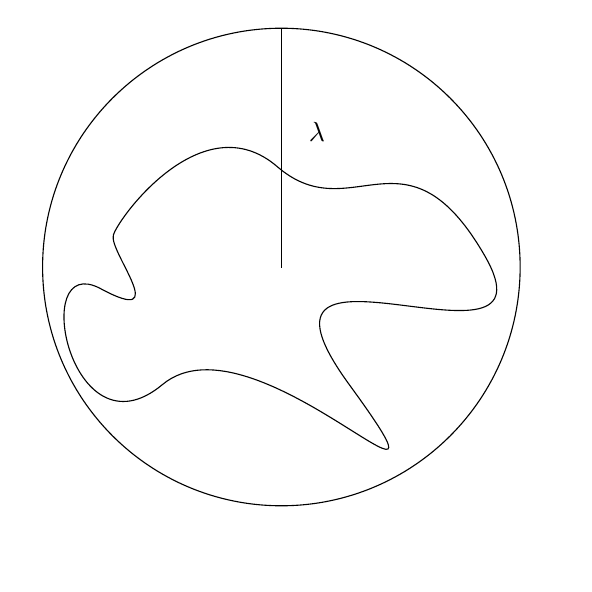
\begin{tikzpicture}[x=0.75pt,y=0.75pt,yscale=-1,xscale=1]

\draw   (266.34,108.02) .. controls (268.59,99.95) and (309.34,44.02) .. (345.34,75.02) .. controls (381.34,106.02) and (407.34,52.02) .. (445.34,118.02) .. controls (483.34,184.02) and (317.34,94.02) .. (380,180) .. controls (442.66,265.98) and (334.34,143.02) .. (290,180) .. controls (245.66,216.98) and (225.34,115.02) .. (260.26,133.81) .. controls (295.19,152.61) and (264.09,116.08) .. (266.34,108.02) -- cycle ;
\draw   (232.26,123.35) .. controls (232.26,59.82) and (283.77,8.31) .. (347.3,8.31) .. controls (410.84,8.31) and (462.34,59.82) .. (462.34,123.35) .. controls (462.34,186.88) and (410.84,238.39) .. (347.3,238.39) .. controls (283.77,238.39) and (232.26,186.88) .. (232.26,123.35) -- cycle ;
\draw    (347.3,8.31) -- (347.3,124.02) ;

\draw (359.33,52.4) node [anchor=north west][inner sep=0.75pt]    {$\lambda$};

\end{tikzpicture}

\end{figure*}

\begin{theorem}{
	Given $S$ is a compact subset of $X$ and $f:X\to\r$ is continuous, then $f$ has a maximum point in $S$.
}
	Since $S$ is compact and $f$ is continuous, $f(S)$ is compact.
	Hence $f(S)$ is closed and bounded.
	Let
	\[
		\alpha \coloneqq \sup(f(S)).
	\]
	Then $\alpha\in f(S)$ since $f(S)$ is closed.
	So there exists $x_0\in S$ such that
	\[
		f(x_0) = \alpha.
	\]
	Therefore $f$ attains a maximum on $S$.
\end{theorem}

\begin{theorem}{
	If $f:X\to Y$ is continuous and $A$ is a compact subset of $X$, then $f$ is uniformly continuous on $A$.
}
	Let $\eps > 0$.
	For each $p\in A$, there exists $\delta_p > 0$ such that
	\[
		d_X(p,x) < \delta_p \implies d_Y(f(p),f(x)) < \frac{\eps}{2}.
	\]
	Consider the open cover
	\[
		\{\vee_{\delta_p/2}(p) : p\in A\}.
	\]
	By compactness, there is a finite subcover
	\[
		\{\vee_{\delta_{p_i}/2}(p_i) : 1 \leq i\leq N\}.
	\]
	Choose
	\[
		\delta \coloneqq \min_{1\leq i\leq N}\frac{\delta_{p_i}}{2}.
	\]
	We show that
	\[
		d_X(x,y) < \delta \implies d_Y(f(x),f(y)) < \eps
	\]
	for all $x,y\in A$.
	Given $x\in A$, choose $p_i$ such that
	\[
		x\in \vee_{\delta_{p_i}/2}(p_i).
	\]
	So
	\[
		d_X(x,p_i) < \frac{\delta_{p_i}}{2}.
	\]
	If also $d_X(x,y) < \delta$, then
	\[
		d_X(x,y) < \frac{\delta_{p_i}}{2}.
	\]
	By the triangle inequality,
	\[
		d_X(y,p_i) \leq d_X(y,x) + d_X(x,p_i) < \frac{\delta_{p_i}}{2} + \frac{\delta_{p_i}}{2} = \delta_{p_i}.
	\]
	Hence both $x$ and $y$ lie in $\vee_{\delta_{p_i}}(p_i)$.
	Therefore
	\[
		d_Y(f(x),f(p_i)) < \frac{\eps}{2}
		\qquad\text{and}\qquad
		d_Y(f(y),f(p_i)) < \frac{\eps}{2}.
	\]
	So
	\[
		d_Y(f(x),f(y)) \leq d_Y(f(x),f(p_i)) + d_Y(f(p_i),f(y)) < \eps.
	\]
	Thus $f$ is uniformly continuous on $A$.
\end{theorem}
%! Author = sriadityavedantam
%! Date = 3/25/26

\lesson{50}{Self-Study Six}{Day 50}

\begin{definition}[Connectedness]
	A metric space $(X,d)$ is connected if it is impossible to write
	\[
		X = U_1\cup U_2
	\]
	as a disjoint union of nonempty open sets with
	\[
		U_1\cap U_2 = \varnothing.
	\]
\end{definition}

\begin{example}[Examples of Connected Sets]
	\[
		\r,\quad \r^n,\quad [a,b].
	\]
\end{example}

\begin{theorem}{
	Let $(X,d_X)$ and $(Y,d_Y)$ be metric spaces and let $f:X\to Y$ be continuous.
	If $X$ is connected, then $f(X)$ is connected.
}
	Suppose, for the sake of contradiction, that $f(X)$ is disconnected.
	Then
	\[
		f(X) = U_1\cup U_2
	\]
	where $U_1,U_2$ are nonempty disjoint open sets in $Y$.
	Then
	\[
		X = f^{-1}(U_1)\cup f^{-1}(U_2).
	\]
	Since $f$ is continuous, $f^{-1}(U_1)$ and $f^{-1}(U_2)$ are open.
	They are disjoint and nonempty.
	This contradicts connectedness of $X$.
	Hence $f(X)$ is connected.
\end{theorem}

\begin{theorem}[Intermediate Value Theorem]{
	Let $X$ be connected and $f:X\to\r$ be continuous.
	If $a,b\in f(X)$ and $a < r < b$, then $r\in f(X)$.
}
	Suppose, for the sake of contradiction, that $r\notin f(X)$.
	Let
	\[
		A \coloneqq (-\infty,r)
		\qquad\text{and}\qquad
		B \coloneqq (r,\infty).
	\]
	Then
	\[
		f(X)\subseteq A\cup B.
	\]
	So
	\[
		X = f^{-1}(A)\cup f^{-1}(B).
	\]
	Both sets are open, disjoint, and nonempty.
	This contradicts connectedness of $X$.
	Hence $r\in f(X)$.
\end{theorem}

\begin{definition}[Directional Derivative]
	Given $U\subset\r^n$ open, $f:U\to\r^m$, $a\in U$, and $u\in\r^n$, define
	\[
		D_u f(a) \coloneqq \lim_{t\to0}\frac{f(a + tu) - f(a)}{t}.
	\]
\end{definition}

\begin{remark}
	In single-variable calculus,
	\[
		f\uptick(a) = \lim_{t\to 0}\frac{f(a + t) - f(a)}{t}.
	\]
	Define $\lambda:\r\to\r$ by
	\[
		\lambda(t) \coloneqq f\uptick(a)t.
	\]
	Then
	\begin{align*}
		\lim_{t\to0}\frac{f(a+t) - f(a) - \lambda(t)}{t}
		&= \lim_{t\to0}\left(\frac{f(a+t) - f(a)}{t} - f\uptick(a)\right)\\
		&= 0.
	\end{align*}
	So for small $t$,
	\[
		f(a+t) - f(a) \approx f\uptick(a)t.
	\]
\end{remark}

\begin{definition}[Differentiability]
	Given $U\subset\r^n$ open and $a\in U$, a function $f:U\to\r^m$ is differentiable at $a$ if there exists a linear map $B:\r^n\to\r^m$ such that
	\[
		\frac{f(a+h) - f(a) - Bh}{\norm{h}}\to 0
		\qquad\text{as } h\to 0.
	\]
	In this case, $Bh$ approximates $f(a+h)-f(a)$.
\end{definition}

\begin{theorem}{
	If $f$ is differentiable at $a$, then for every $u\in\r^n$, the directional derivative $D_u f(a)$ exists and
	\[
		D_u f(a) = Bu.
	\]
}
	Since $f$ is differentiable at $a$,
	\[
		\frac{f(a+tu) - f(a) - B(tu)}{\norm{tu}}\to 0
		\qquad\text{as } t\to 0.
	\]
	Then
	\begin{align*}
		\frac{f(a+tu) - f(a)}{t}
		&= \frac{B(tu)}{t} + \frac{f(a+tu) - f(a) - B(tu)}{t}\\
		&= Bu + \frac{f(a+tu) - f(a) - B(tu)}{t}.
	\end{align*}
	The second term goes to $0$ as $t\to 0$.
	Hence
	\[
		\frac{f(a+tu) - f(a)}{t}\to Bu.
	\]
\end{theorem}

\begin{remark}
	We use $Df(a)$ to denote the derivative.
\end{remark}

\section{Lebesgue's Criterion for Riemann Integrability}

\begin{observation}
	The following is Thomae's function.
	It is continuous at every irrational point and discontinuous at every rational point.
	Nevertheless, it is Riemann integrable on $[0,1]$ with
	\begin{gather*}
	    \int_0^1 t(x)\,dx = 0.\\
	    t(x) =
		\begin{cases}
			1, & x=0,\\
			1/n, & x=m/n\in\q\setminus\{0\}\text{ in lowest terms},\\
			0, & x\notin\q.
		\end{cases}\\
	\end{gather*}
\end{observation}

\begin{definition}[Measure Zero]
	A set $A$ has measure zero if for all $\eps > 0$, there exists a countable collection of open intervals $\{O_n\}$ such that
	\[
		A\subseteq\bigcup_{n=1}^\infty O_n
		\qquad\text{and}\qquad
		\sum_{n=1}^\infty\abs{O_n}\leq\eps.
	\]
\end{definition}

\begin{theorem}[Lebesgue's Theorem]{
	Let $f$ be bounded on $[a,b]$.
	Then $f$ is Riemann integrable if and only if the set of discontinuities has measure zero.
}
	Let $M>0$ such that $\abs{f(x)}\leq M$ for all $x\in[a,b]$.
	Define
	\begin{gather*}
	    D \coloneqq \{x\in[a,b] : \text{$f$ is not continuous at $x$}\}.\\
	    D^\alpha \coloneqq \{x\in[a,b] : \text{$f$ is not $\alpha$-continuous at $x$}\}.\\
	\end{gather*}

	\textbf{($\impliedby$).}
	Suppose $D$ has measure zero.
	Let $\eps > 0$ and set
	\[
		\alpha \coloneqq \frac{\eps}{2(b-a)}.
	\]
	\begin{problem}
		Show there exists a finite collection of disjoint open intervals $\{G_1,\ldots,G_N\}$ covering $D^\alpha$ such that
		\[
			\sum_{n=1}^N \abs{G_n} < \frac{\eps}{4M}.
		\]
	\end{problem}
	\begin{problem}
		Let $K \coloneqq [a,b]\setminus \bigcup_{n=1}^N G_n$.
		Show $f$ is uniformly $\alpha$-continuous on $K$.
	\end{problem}

	\begin{problem}
		Construct a partition $P_\eps$ such that
		\[
			U(f,P_\eps)-L(f,P_\eps)\leq \eps.
		\]
	\end{problem}

	\textbf{($\implies$).}
	Suppose $f$ is Riemann integrable.
	Given $\eps > 0$ and $\alpha > 0$, choose a partition $P_\eps$ such that
	\[
		U(f,P_\eps)-L(f,P_\eps) < \alpha\eps.
	\]

	\begin{problem}
		(a) Show $D^\alpha$ has measure zero.

		(b) Deduce $D$ has measure zero.
	\end{problem}
\end{theorem}

\chapter{Problem Sets}

%! Author = sriadityavedantam
%! Date = 3/25/26

\section{Homework 0}

\begin{problem}{
    \label{ex:0.1}
    The transitive property for the rationals holds: if $(a,b)\sim(\alpha,\beta)$ and $(\alpha,\beta)\sim(c,d)$, then $(a,b)\sim(c,d)$.
}
    Assume
    \[
        (a,b)\sim(\alpha,\beta)
        \qquad\text{and}\qquad
        (\alpha,\beta)\sim(c,d).
    \]
    By definition,
    \[
        a\beta=\alpha b
        \qquad\text{and}\qquad
        \alpha d=\beta c.
    \]
    Multiply the two equations:
    \[
        (a\beta)(\alpha d)=(\alpha b)(\beta c).
    \]
    Cancel the common factors:
    \[
        (a\cancel{\beta})(\cancel{\alpha}d)=(\cancel{\alpha}b)(\cancel{\beta}c).
    \]
    Hence
    \[
        ad=bc.
    \]
    Therefore
    \[
        (a,b)\sim(c,d).
    \]
\end{problem}

\begin{problem}[Lemma 1.6 --- Transitivity Proof]{
    The transitive property for the rationals holds if $(a,b)\sim(\alpha,\beta)$ and $(\alpha,\beta)\sim(c,d)$, then $(a,b)\sim(c,d)$.
}
    Assume
    \[
        a\beta=\alpha b
        \qquad\text{and}\qquad
        \alpha d=\beta c.
    \]
    Then
    \begin{align*}
        (a\beta)(\alpha d)
&=(\alpha b)(\beta c)\\
(a\cancel{\beta})(\cancel{\alpha}d)
&=(\cancel{\alpha}b)(\cancel{\beta}c)\\
ad&=bc.
    \end{align*}
    Hence $(a,b)\sim(c,d)$.
\end{problem}

\begin{problem}[Proposition 1.8 --- Addition is Well-Defined]{
    Given $(a,b)\sim(c,d)$ and $(\alpha,\beta)\sim(\gamma,\delta)$, show
    \[
        (a\beta+\alpha b,\,b\beta)\sim(c\delta+\gamma d,\,d\delta).
    \]
    This is how addition is defined:
    \[
        (a,b)+(\alpha,\beta)\coloneqq (a\beta+\alpha b,\,b\beta).
    \]
}
    From the relations,
    \[
        ad=bc
        \qquad\text{and}\qquad
        \alpha\delta=\beta\gamma.
    \]
    We compute
    \begin{align*}
        (a\beta+\alpha b)(d\delta)
&=a\beta d\delta+\alpha bd\delta\\
&=(ad)(\beta\delta)+(\alpha\delta)(bd).
    \end{align*}
    Using $ad=bc$ and $\alpha\delta=\beta\gamma$, this becomes
    \begin{align*}
        (ad)(\beta\delta)+(\alpha\delta)(bd)
    &=(bc)(\beta\delta)+(\beta\gamma)(bd)\\
        &=b\beta(c\delta+\gamma d).
    \end{align*}
    Therefore
    \[
        (a\beta+\alpha b)(d\delta)=(c\delta+\gamma d)(b\beta),
    \]
    so
    \[
        (a\beta+\alpha b,\,b\beta)\sim(c\delta+\gamma d,\,d\delta).
    \]
    Hence addition is well-defined.
\end{problem}

\begin{problem}{
    Why must we use $\z\times(\z\setminus\{0\})$?
    Show that the relation
    \[
        (a,b)\sim(c,d)\iff ad=bc
    \]
    is not an equivalence relation on $\z\times\z$.
}
    Suppose this relation is defined on $\z\times\z$.
    Take
    \[
        (a,b)=(1,0),\qquad (c,d)=(1,0),\qquad (e,f)=(1,1).
    \]
    Then
    \[
        (1,0)\sim(1,0)
    \]
    because
    \[
        1\cdot 0=0\cdot 1.
    \]
    Also
    \[
        (1,0)\sim(1,1)
    \]
    because
    \[
        1\cdot 1=0\cdot 1
    \]
    is false, so this choice does not work.
    Instead take
    \[
        (a,b)=(1,0),\qquad (c,d)=(0,0),\qquad (e,f)=(0,1).
    \]
    Then
    \[
        (1,0)\sim(0,0)
    \]
    because
    \[
        1\cdot 0=0\cdot 0.
    \]
    Also
    \[
        (0,0)\sim(0,1)
    \]
    because
    \[
        0\cdot 1=0\cdot 0.
    \]
    But
    \[
        (1,0)\not\sim(0,1)
    \]
    because
    \[
        1\cdot 1\neq 0\cdot 0.
    \]
    So transitivity fails.
    Hence this is not an equivalence relation on $\z\times\z$.
    This is why the second component must be nonzero.
\end{problem}
%! Author = sriadityavedantam
%! Date = 3/25/26

\section{Homework 1}

\begin{problem}[Greatest Lower Bound Property of $\rr$]{
    Deduce the g.l.b.\ property from the l.u.b.\ property.
    Let $S\subset\rr$ and suppose $S$ is bounded below.
    Show that
    \[
        \inf(S)=-\sup\{-x:x\in S\}.
    \]
}
    Let
    \[
        R\coloneqq\{-x:x\in S\}.
    \]
    Because $S$ is bounded below, $R$ is bounded above.
    By the l.u.b.\ property of $\rr$, there exists
    \[
        \alpha\coloneqq\sup(R).
    \]
    Since $\alpha\geq r$ for all $r\in R$, we have
    \[
        \alpha\geq -s
        \qquad\text{for all } s\in S.
    \]
    Thus
    \[
        -\alpha\leq s
        \qquad\text{for all } s\in S,
    \]
    so $-\alpha$ is a lower bound of $S$.
    Now let $\beta$ be any lower bound of $S$.
    Then
    \[
        \beta\leq s
        \qquad\text{for all } s\in S,
    \]
    so
    \[
        -\beta\geq -s
        \qquad\text{for all } s\in S.
    \]
    Hence $-\beta$ is an upper bound of $R$.
    Since $\alpha=\sup(R)$, we have
    \[
        \alpha\leq -\beta.
    \]
    Therefore
    \[
        -\alpha\geq \beta.
    \]
    So $-\alpha$ is greater than or equal to every lower bound of $S$.
    Hence
    \[
        \inf(S)=-\alpha=-\sup\{-x:x\in S\}.
    \]
\end{problem}

\begin{problem}[Lemma 1.6 --- Ordering of Squares]{
    Suppose $a,b\in\rr$ and $a,b>0$.
    Then $a^2<b^2$ if and only if $a<b$.
}
    Assume
    \[
        a^2<b^2.
    \]
    Then
    \[
        0<b^2-a^2=(b-a)(b+a).
    \]
    Because $b+a>0$, it follows that
    \[
        b-a>0.
    \]
    Hence
    \[
        a<b.
    \]
    Conversely, if $a<b$, then since $a+b>0$,
    \[
        (b-a)(b+a)>0.
    \]
    Thus
    \[
        b^2-a^2>0,
    \]
    so
    \[
        a^2<b^2.
    \]
    Therefore
    \[
        a^2<b^2 \iff a<b.
    \]
\end{problem}
%! Author = sriadityavedantam
%! Date = 3/25/26

\section{Homework 2}

\begin{problem}[Subsets of Uncountable Sets]{
    \begin{enumerate}[label={(\alph*)}]
\item Let $C\subseteq[0,1]$ be uncountable.
Show there exists $a\in(0,1)$ such that $C\cap[a,1]$ is uncountable.
\item Let $A$ be the set of all $a\in(0,1)$ such that $C\cap[a,1]$ is uncountable, and define $\alpha=\sup(A)$.
Is $C\cap[\alpha,1]$ uncountable?
\item Does the statement in \textbf{(a)} remain true if “uncountable” is replaced by “infinite”?
    \end{enumerate}
}
    \textbf{(a).}
    For each $n\in\n$, define
    \[
        A_n\coloneqq C\cap\left[\frac{1}{n+1},1\right].
    \]
    Then
    \[
        \bigcup_{n=1}^\infty A_n=C\setminus\bigl(C\cap\{0\}\bigr).
    \]
    The set $C\cap\{0\}$ has at most one element, so if every $A_n$ were countable, then the countable union
    \[
        \bigcup_{n=1}^\infty A_n
    \]
    would be countable, and adjoining at most one point would still give a countable set.
    That would imply $C$ is countable, a contradiction.
    Hence some $A_n$ is uncountable.
    Set
    \[
        a\coloneqq\frac{1}{n+1}\in(0,1).
    \]
    Then
    \[
        C\cap[a,1]
    \]
    is uncountable.

    \textbf{(b).}
    Not necessarily.
    Take
    \[
        C=[0,1).
    \]
    Then for every $a\in(0,1)$,
    \[
        C\cap[a,1]=[a,1)
    \]
    is uncountable, so
    \[
        A=(0,1)
    \]
    and hence
    \[
        \alpha=\sup(A)=1.
    \]
    But then
    \[
        C\cap[\alpha,1]=C\cap[1,1]=\varnothing,
    \]
    which is not uncountable.
    So the answer is no.

    \textbf{(c).}
    No.
    Take
    \[
        C=\left\{\frac{1}{n}:n\in\n\right\}\subset[0,1].
    \]
    Then $C$ is infinite, but for every $a\in(0,1)$,
    \[
        C\cap[a,1]
    \]
    is finite.
    So the statement fails if “uncountable” is replaced by “infinite.”
\end{problem}

\begin{problem}[Arithmetic of Suprema]{
    Let $A,B\subset\rr$ be nonempty sets that are bounded above.
    \begin{enumerate}[label={(\alph*)}]
\item Define
\[
    C\coloneqq\{x:x=a+b\text{ for some }a\in A,\ b\in B\}.
\]
Show that
\[
    \sup(C)=\sup(A)+\sup(B).
\]
\item Show there exists a monotonically increasing sequence $(x_n)$, with all $x_n\in A$, such that $x_n\to\sup(A)$.
    \end{enumerate}
}
    \textbf{(a).}
    Let
    \[
        \alpha\coloneqq\sup(A)
        \qquad\text{and}\qquad
        \beta\coloneqq\sup(B).
    \]
    For all $a\in A$ and $b\in B$,
    \[
        a\leq\alpha
        \qquad\text{and}\qquad
        b\leq\beta.
    \]
    Hence
    \[
        a+b\leq\alpha+\beta.
    \]
    So $\alpha+\beta$ is an upper bound for $C$, and therefore
    \[
        \sup(C)\leq\alpha+\beta.
    \]
    Now let $\eps>0$.
    Since $\alpha=\sup(A)$, there exists $\gamma\in A$ such that
    \[
        \gamma>\alpha-\frac{\eps}{2}.
    \]
    Since $\beta=\sup(B)$, there exists $\delta\in B$ such that
    \[
        \delta>\beta-\frac{\eps}{2}.
    \]
    Then
    \[
        \gamma+\delta>\alpha+\beta-\eps.
    \]
    Because $\gamma+\delta\in C$, we have
    \[
        \sup(C)\geq\gamma+\delta>\alpha+\beta-\eps.
    \]
    Since this holds for all $\eps>0$,
    \[
        \sup(C)\geq\alpha+\beta.
    \]
    Thus
    \[
        \sup(C)=\alpha+\beta.
    \]

    \textbf{(b).}
    Let
    \[
        \alpha\coloneqq\sup(A).
    \]
    For each $n\in\n$, since $\alpha-\frac1n$ is not an upper bound of $A$, there exists $a_n\in A$ such that
    \[
        \alpha-\frac1n<a_n\leq\alpha.
    \]
    Now define
    \[
        x_1\coloneqq a_1,
        \qquad
        x_n\coloneqq\max\{x_{n-1},a_n\}\quad\text{for }n\geq2.
    \]
    Then each $x_n\in A$, and $(x_n)$ is monotonically increasing.
    Also
    \[
        x_n\leq\alpha
        \qquad\text{for all }n.
    \]
    Let $\eps>0$.
    Choose $N\in\n$ such that
    \[
        \frac1N<\eps.
    \]
    Then
    \[
        a_N>\alpha-\eps.
    \]
    Since $x_n\geq a_N$ for all $n\geq N$,
    \[
        \alpha-\eps<x_n\leq\alpha
        \qquad\text{for all }n\geq N.
    \]
    Thus
    \[
        \abs{x_n-\alpha}<\eps
        \qquad\text{for all }n\geq N.
    \]
    Hence
    \[
        x_n\to\alpha=\sup(A).
    \]
\end{problem}

\begin{problem}[Limits of a Root]{
    Let $x_n\geq0$ for all $n\in\n$.
    \begin{enumerate}[label={(\alph*)}]
\item If $(x_n)\to0$, show that $(\sqrt{x_n})\to0$.
\item If $(x_n)\to x$, show that $(\sqrt{x_n})\to\sqrt{x}$.
    \end{enumerate}
}
    \textbf{(a).}
    Let $\eps>0$.
    Because $x_n\to0$, there exists $N\in\n$ such that for all $n\geq N$,
    \[
        \abs{x_n}<\eps^2.
    \]
    Since $x_n\geq0$,
    \[
        0\leq x_n<\eps^2.
    \]
    Taking square roots gives
    \[
        0\leq \sqrt{x_n}<\eps.
    \]
    Hence
    \[
        \abs{\sqrt{x_n}-0}<\eps
    \]
    for all $n\geq N$.
    So
    \[
        \sqrt{x_n}\to0.
    \]

    \textbf{(b).}
    Since $x_n\geq0$ for all $n$ and $x_n\to x$, we must have $x\geq0$.
    Now
    \[
        \abs{\sqrt{x_n}-\sqrt{x}}
        =
        \frac{\abs{x_n-x}}{\sqrt{x_n}+\sqrt{x}}.
    \]
    If $x=0$, then this is part \textbf{(a)}.
    So assume $x>0$.
    Choose $N_1$ such that for $n\geq N_1$,
    \[
        \abs{x_n-x}<\frac{x}{2}.
    \]
    Then for $n\geq N_1$,
    \[
        x_n>\frac{x}{2},
    \]
    so
    \[
        \sqrt{x_n}+\sqrt{x}\geq \sqrt{x}.
    \]
    Hence
    \[
        \abs{\sqrt{x_n}-\sqrt{x}}
        \leq \frac{\abs{x_n-x}}{\sqrt{x}}.
    \]
    Now let $\eps>0$.
    Choose $N_2$ such that for $n\geq N_2$,
    \[
        \abs{x_n-x}<\eps\sqrt{x}.
    \]
    Then for $n\geq \max\{N_1,N_2\}$,
    \[
        \abs{\sqrt{x_n}-\sqrt{x}}<\eps.
    \]
    Therefore
    \[
        \sqrt{x_n}\to\sqrt{x}.
    \]
\end{problem}

\begin{problem}[Examples of Limit Convergence]{
    Using only the definition of convergence, prove that if $x_n\to2$, then
    \begin{enumerate}[label={(\alph*)}]
\item \(\left(\frac{2x_n-1}{3}\right)\to1\),
\item \(\left(\frac{1}{x_n}\right)\to\frac12\).
    \end{enumerate}
}
    \textbf{(a).}
    Let $\eps>0$.
    Since $x_n\to2$, there exists $N\in\n$ such that for all $n\geq N$,
    \[
        \abs{x_n-2}<\frac{3\eps}{2}.
    \]
    Then
    \begin{align*}
        \abs{\frac{2x_n-1}{3}-1}
        &=\abs{\frac{2x_n-4}{3}}\\
        &=\frac23\abs{x_n-2}\\
        &<\frac23\cdot\frac{3\eps}{2}\\
        &=\eps.
    \end{align*}
    Hence
    \[
        \frac{2x_n-1}{3}\to1.
    \]

    \textbf{(b).}
    Let $\eps>0$.
    Since $x_n\to2$, there exists $N_1$ such that for all $n\geq N_1$,
    \[
        \abs{x_n-2}<1.
    \]
    Then for $n\geq N_1$,
    \[
        1<x_n<3,
    \]
    so in particular
    \[
        x_n\geq1.
    \]
    Also choose $N_2$ such that for all $n\geq N_2$,
    \[
        \abs{x_n-2}<2\eps.
    \]
    Now for $n\geq\max\{N_1,N_2\}$,
    \begin{align*}
        \abs{\frac1{x_n}-\frac12}
        &=\abs{\frac{2-x_n}{2x_n}}\\
        &=\frac{\abs{x_n-2}}{2x_n}\\
        &\leq \frac{\abs{x_n-2}}{2}\\
        &<\frac{2\eps}{2}\\
        &=\eps.
    \end{align*}
    Hence
    \[
        \frac1{x_n}\to\frac12.
    \]
\end{problem}

\begin{problem}[Cesàro Means]{
    \begin{enumerate}[label={(\alph*)}]
\item Show that if $(x_n)$ converges to $L$, then the averages
\[
    y_n=\frac{x_1+x_2+\cdots+x_n}{n}
\]
also converge to $L$.
\item Give an example where $(y_n)$ converges even though $(x_n)$ does not.
    \end{enumerate}
}
    \textbf{(a).}
    Assume $x_n\to L$.
    Let
    \[
        y_n=\frac{x_1+\cdots+x_n}{n}.
    \]
    Then
    \[
        y_n-L=\frac{(x_1-L)+\cdots+(x_n-L)}{n}.
    \]
    Let $\eps>0$.
    Choose $N$ such that for all $n\geq N$,
    \[
        \abs{x_n-L}<\eps.
    \]
    Then
    \begin{align*}
        \abs{y_n-L}
        &\leq \frac1n\sum_{k=1}^n \abs{x_k-L}\\
        &= \frac1n\sum_{k=1}^{N-1}\abs{x_k-L}
        +\frac1n\sum_{k=N}^{n}\abs{x_k-L}\\
        &< \frac{C}{n}+\frac{n-N+1}{n}\eps,
    \end{align*}
    where
    \[
        C\coloneqq \sum_{k=1}^{N-1}\abs{x_k-L}.
    \]
    Since $\frac{C}{n}\to0$ and $\frac{n-N+1}{n}\leq1$, it follows that
    \[
        \abs{y_n-L}\to0.
    \]
    Hence
    \[
        y_n\to L.
    \]

    \textbf{(b).}
    Take
    \[
        x_n=(-1)^n.
    \]
    Then $(x_n)$ does not converge.
    But the averages satisfy
    \[
        y_{2k}=0
        \qquad\text{and}\qquad
        y_{2k+1}=-\frac{1}{2k+1}.
    \]
    So
    \[
        y_n\to0.
    \]
\end{problem}
%! Author = sriadityavedantam
%! Date = 3/25/26

\section{Homework 3}

\begin{problem}[Infinite Products]{
    Consider
    \[
        \prod_{n=1}^\infty(1+a_n)
        \qquad\text{where } a_n\geq0.
    \]

    \begin{enumerate}[label={(\alph*)}]
\item Find an explicit formula for the partial products when $a_n=1/n$ and decide whether they converge.
Also examine the case $a_n=1/n^2$.
\item Show that the partial products converge if and only if $\sum a_n$ converges.
    \end{enumerate}
}
    \textbf{(a).}
    If $a_n=\frac1n$, then
    \[
        p_m=\prod_{n=1}^m\left(1+\frac1n\right)
        =\prod_{n=1}^m \frac{n+1}{n}.
    \]

    This telescopes:
    \[
        p_m=\frac21\cdot\frac32\cdots\frac{m+1}{m}=m+1.
    \]

    Hence
    \[
        p_m\to\infty,
    \]
    so the product diverges.

    If $a_n=\frac1{n^2}$, then
    \[
        p_m=\prod_{n=1}^m\left(1+\frac1{n^2}\right).
    \]

    The first few terms are
    \[
        2,\quad 2\cdot\frac54,\quad 2\cdot\frac54\cdot\frac{10}{9},\quad \ldots
    \]

    This suggests convergence.

    \textbf{(b).}
    Assume first that
    \[
        \sum_{n=1}^\infty a_n
    \]
    converges.

    Let
    \[
        s_m=\sum_{n=1}^m a_n.
    \]

    Since $a_n\geq0$, the sequence $(s_m)$ is bounded.

    Also
    \[
        1+a_n\leq 3^{a_n}
    \]
    for $a_n\geq0$.

    Thus
    \[
        p_m=\prod_{n=1}^m(1+a_n)\leq \prod_{n=1}^m 3^{a_n}=3^{s_m}.
    \]

    So $(p_m)$ is bounded above.

    Because each factor $1+a_n\geq1$, $(p_m)$ is increasing.

    Hence $(p_m)$ converges.

    Conversely, assume $(p_m)$ converges.

    Then $(p_m)$ is bounded.

    We claim
    \[
        p_m\geq 1+\sum_{n=1}^m a_n.
    \]

    This is true by induction.

    For $m=1$,
    \[
        p_1=1+a_1.
    \]

    If it holds for $m$, then
    \begin{align*}
        p_{m+1}
        &=p_m(1+a_{m+1})\\
        &\geq \left(1+\sum_{n=1}^m a_n\right)(1+a_{m+1})\\
        &\geq 1+\sum_{n=1}^{m+1}a_n.
    \end{align*}

    Thus
    \[
        1+\sum_{n=1}^m a_n\leq p_m.
    \]

    Since $(p_m)$ is bounded, the partial sums of $\sum a_n$ are bounded.

    Because $a_n\geq0$, the partial sums are increasing.

    Hence
    \[
        \sum_{n=1}^\infty a_n
    \]
    converges.
\end{problem}

\begin{problem}[Infinite Products Two]{
    \begin{enumerate}[label={(\alph*)}]
\item Does
\[
    \frac21\cdot\frac32\cdot\frac54\cdot\frac98\cdot\frac{17}{16}\cdots
\]
converge?
\item Does
\[
    \frac12\cdot\frac34\cdot\frac56\cdot\frac78\cdot\frac9{10}\cdots
\]
converge to zero?
\item Show that
\[
    \left(\frac{2\cdot2}{1\cdot3}\right)\left(\frac{4\cdot4}{3\cdot5}\right)\left(\frac{6\cdot6}{5\cdot7}\right)\cdots
\]
at least converges.
    \end{enumerate}
}
    \textbf{(a).}
    This product is
    \[
        \prod_{n=1}^\infty\left(1+\frac{1}{2^n}\right).
    \]

    Using the identity
    \[
        \prod_{n=1}^m\left(1+\frac{1}{2^n}\right)=\frac{2-2^{-m}}{1},
    \]
    or by the standard telescoping trick,
    \[
        p_m=2-\frac{1}{2^m}.
    \]

    Hence
    \[
        p_m\to2.
    \]

    So the product converges.

    \textbf{(b).}
    This product is
    \[
        \prod_{k=1}^\infty \frac{2k-1}{2k}
        =
        \prod_{k=1}^\infty\left(1-\frac{1}{2k}\right).
    \]

    Each factor lies in $(0,1)$, so the partial products are decreasing and bounded below by $0$.

    Hence they converge.

    To determine the limit, note that
    \[
        \frac{1}{\prod_{k=1}^n \frac{2k-1}{2k}}
        =
        \prod_{k=1}^n \left(1+\frac{1}{2k-1}\right).
    \]

    But
    \[
        \sum_{k=1}^\infty \frac{1}{2k-1}
    \]
    diverges, so by the previous problem the reciprocal product diverges to $\infty$.

    Hence the original product converges to $0$.

    \textbf{(c).}
    The Wallis product can be written as
    \[
        \prod_{n=1}^\infty \frac{4n^2}{4n^2-1}
        =
        \prod_{n=1}^\infty \left(1+\frac{1}{4n^2-1}\right).
    \]

    Since
    \[
        0<\frac{1}{4n^2-1}\leq \frac{1}{n^2},
    \]
    and
    \[
        \sum_{n=1}^\infty \frac{1}{n^2}
    \]
    converges, it follows by comparison that
    \[
        \sum_{n=1}^\infty \frac{1}{4n^2-1}
    \]
    converges.

    Therefore the infinite product converges.
\end{problem}

\begin{problem}[Iterated Series]{
    Show that if
    \[
        \sum_{i=1}^{\infty}\sum_{j=1}^{\infty}\abs{a_{ij}}
    \]
    converges, then
    \[
        \sum_{i=1}^{\infty}\sum_{j=1}^{\infty} a_{ij}
    \]
    converges.
}
    For each fixed $i$, the series
    \[
        \sum_{j=1}^\infty \abs{a_{ij}}
    \]
    converges.

    Hence
    \[
        \sum_{j=1}^\infty a_{ij}
    \]
    converges absolutely, and therefore converges.

    Let
    \[
        b_i\coloneqq \sum_{j=1}^\infty \abs{a_{ij}}
        \qquad\text{and}\qquad
        c_i\coloneqq \sum_{j=1}^\infty a_{ij}.
    \]

    Then
    \[
        \abs{c_i}\leq b_i.
    \]

    Since
    \[
        \sum_{i=1}^\infty b_i
    \]
    converges, comparison implies
    \[
        \sum_{i=1}^\infty c_i
    \]
    converges.

    Thus
    \[
        \sum_{i=1}^{\infty}\sum_{j=1}^{\infty} a_{ij}
    \]
    converges.
\end{problem}
%! Author = sriadityavedantam
%! Date = 3/25/26

\section{Homework 4}

\begin{problem}{
    Decide whether the following sets are open, closed, or neither.
    If a set is not open, find a point in the set for which there is no $\eps$-neighborhood contained in the set.
    If a set is not closed, find a limit point that is not contained in the set.
    \begin{enumerate}[label={(\arabic*)}]
	\item $\q$
    \item $\n$
    \item $\{x\in\r : x\neq 0\}$
    \item $\left\{1+\frac14+\frac19+\cdots+\frac1{n^2} : n\in\n\right\}$
    \item $\left\{1+\frac12+\frac13+\cdots+\frac1n : n\in\n\right\}$
    \end{enumerate}
}
    \begin{enumerate}[label={(\arabic*)}]
	\item $\q$ is neither open nor closed.

    It is not open because if $q\in\q$ and $\eps>0$, then $(q-\eps,q+\eps)$ contains irrational numbers, so no $\eps$-neighborhood of $q$ lies in $\q$.

    It is not closed because $\sqrt{2}$ is a limit point of $\q$ but $\sqrt{2}\notin\q$.

    \item $\n$ is closed but not open.

    It is not open because if $n\in\n$ and $\eps>0$, then $(n-\eps,n+\eps)$ contains non-natural numbers.

    It is closed because every point of $\n$ is isolated, so $\n$ has no limit points in $\r$ outside itself.

    \item $\{x\in\r : x\neq 0\}$ is open but not closed.

    Indeed,
    \[
        \{x\in\r : x\neq 0\} = (-\infty,0)\cup(0,\infty),
    \]
    which is open.

    It is not closed because $0$ is a limit point and $0$ is not in the set.

    \item Let
    \[
        S_4 \coloneqq \left\{1+\frac14+\frac19+\cdots+\frac1{n^2} : n\in\n\right\}.
    \]

    This set is not open because each point is isolated.

    It is not closed because the sequence of its elements converges to
    \[
        \sum_{n=1}^\infty \frac1{n^2} = \frac{\pi^2}{6},
    \]
    and $\frac{\pi^2}{6}\notin S_4$.

    \item Let
    \[
        S_5 \coloneqq \left\{1+\frac12+\frac13+\cdots+\frac1n : n\in\n\right\}.
    \]

    This set is not open because each point is isolated.

    It is closed because the harmonic partial sums diverge to $+\infty$, so $S_5$ has no finite limit points.
    \end{enumerate}
\end{problem}

\begin{problem}{
    Let $A$ be nonempty and bounded above so that $s=\sup(A)$ exists.
    \begin{enumerate}[label={(\alph*)}]
	\item Show that $s\in\overline{A}$.
    \item Can an open set contain its supremum?
    \end{enumerate}
}
    \textbf{(a).}
    Let $\eps>0$.

    Because $s=\sup(A)$, the number $s-\eps$ is not an upper bound for $A$.

    So there exists $a\in A$ such that
    \[
        s-\eps<a\leq s.
    \]

    Hence
    \[
        \abs{a-s}<\eps.
    \]

    Therefore every $\eps$-neighborhood of $s$ meets $A$, so
    \[
        s\in\overline{A}.
    \]

    \textbf{(b).}
    Yes.

    For example, let
    \[
        A=(0,1)
    \]
    and let
    \[
        U=(-1,2).
    \]

    Then $U$ is open and contains $\sup(A)=1$.
\end{problem}

\begin{problem}{
    Decide whether the following statements are true or false.
    Provide counterexamples for those that are false, and supply proofs for those that are true.
    \begin{enumerate}[label={(\alph*)}]
	\item An open set that contains every rational number must necessarily be all of $\r$.
    \item The Nested Interval Property remains true if the term “closed interval” is replaced by “closed set.”
    \item Every nonempty open set contains a rational number.
    \item Every bounded infinite closed set contains a rational number.
    \item The Cantor set is closed.
    \end{enumerate}
}
    \textbf{(a).} False.

    Take
    \[
        \r\setminus\{\sqrt{2}\}.
    \]

    This set is open, contains every rational number, but is not all of $\r$.

    \textbf{(b).} False.

    Take
    \[
        F_n \coloneqq \{n,n+1,n+2,\ldots\}.
    \]

    Each $F_n$ is closed, the family is nested, and each $F_n$ is nonempty.
    But
    \[
        \bigcap_{n=1}^\infty F_n = \varnothing.
    \]

    \textbf{(c).} True.

    Let $U$ be a nonempty open set and choose $x\in U$.
    Then there exists $\eps>0$ such that
    \[
        (x-\eps,x+\eps)\subseteq U.
    \]

    Because $\q$ is dense in $\r$, there exists $q\in\q$ such that
    \[
        q\in(x-\eps,x+\eps).
    \]

    Hence $q\in U$.

    \textbf{(d).} False.

    Take
    \[
        S\coloneqq \left\{\sqrt{2}+\frac1n : n\in\n\right\}\cup\{\sqrt{2}\}.
    \]

    This set is bounded, infinite, and closed, but it contains no rational number.

    \textbf{(e).} True.

    The Cantor set is an intersection of closed sets, so it is closed.
\end{problem}

\begin{problem}{
    Assume $A$ is an open set and $B$ is a closed set.
    Determine if the following sets are definitely open, definitely closed, both, or neither.
    \begin{enumerate}[label={(\alph*)}]
	\item $\overline{A\cup B}$
    \item $A\setminus B = \{x\in A : x\notin B\}$
    \item $(A^c\cup B)^c$
    \item (A \cap B)\cup(A^c \cap B)
    \item $\overline{A}^{\,c}\cap \overline{A^c}$
    \end{enumerate}
}
    \textbf{(a).}
    \[
        \overline{A\cup B}
    \]
    is definitely closed.

    It need not be open.

    \textbf{(b).}
    Since $B$ is closed, $B^c$ is open.
    Thus
    \[
        A\setminus B = A\cap B^c
    \]
    is an intersection of two open sets, hence is open.

    \textbf{(c).}
    By De Morgan's law,
    \[
        (A^c\cup B)^c = A\cap B^c.
    \]

    By part \textbf{(b)}, this is open.

    \textbf{(d).}
    Factor out $B$:
    \[
        (A\cap B)\cup(A^c\cap B) = (A\cup A^c)\cap B = \r\cap B = B.
    \]

    So this set is definitely closed.

    \textbf{(e).}
    Since $A$ is open, $A^c$ is closed, so
    \[
        \overline{A^c}=A^c.
    \]

    Also
    \[
        \overline{A}^{\,c}\subseteq A^c.
    \]

    Hence
    \[
        \overline{A}^{\,c}\cap\overline{A^c}
        =
        \overline{A}^{\,c}\cap A^c
        =
        \overline{A}^{\,c}.
    \]

    Because $\overline{A}$ is closed, $\overline{A}^{\,c}$ is open.

    So the set is definitely open.
\end{problem}

\begin{problem}{
    \begin{enumerate}[label={(\alph*)}]
	\item Prove that
    \[
        \overline{A\cup B}=\overline{A}\cup\overline{B}.
    \]
    \item Does this result about closures extend to infinite unions of sets?
    \end{enumerate}
}
    \textbf{(a).}
    Because
    \[
        A\subseteq \overline{A}
        \qquad\text{and}\qquad
        B\subseteq \overline{B},
    \]
    we have
    \[
        A\cup B\subseteq \overline{A}\cup\overline{B}.
    \]

    Since $\overline{A}\cup\overline{B}$ is closed, it follows that
    \[
        \overline{A\cup B}\subseteq \overline{A}\cup\overline{B}.
    \]

    Conversely,
    \[
        A\subseteq A\cup B
        \qquad\text{and}\qquad
        B\subseteq A\cup B,
    \]
    so
    \[
        \overline{A}\subseteq \overline{A\cup B}
        \qquad\text{and}\qquad
        \overline{B}\subseteq \overline{A\cup B}.
    \]

    Hence
    \[
        \overline{A}\cup\overline{B}\subseteq \overline{A\cup B}.
    \]

    Therefore
    \[
        \overline{A\cup B}=\overline{A}\cup\overline{B}.
    \]

    \textbf{(b).}
    No.

    For example, let
    \[
        A_n \coloneqq \left\{\frac1n\right\}.
    \]

    Then each $A_n$ is closed, so
    \[
        \bigcup_{n=1}^\infty \overline{A_n}
        =
        \left\{\frac1n : n\in\n\right\}.
    \]

    But
    \[
        \overline{\bigcup_{n=1}^\infty A_n}
        =
        \left\{\frac1n : n\in\n\right\}\cup\{0\}.
    \]

    So the equality fails for infinite unions.
\end{problem}

\begin{definition}[Connectedness]
    Given a metric space $(X,d)$, we say $X$ is connected if it is impossible to write
    \[
        X = U_1\cup U_2
    \]
    as a disjoint union of nonempty open sets such that
    \[
        U_1\cap U_2 = \varnothing.
    \]
\end{definition}

\begin{example}[Examples of Connected Sets]
    \[
        \r,\qquad \r^n,\qquad [a,b].
    \]
\end{example}

\begin{problem}{
    Prove that the only sets that are both open and closed are $\r$ and $\varnothing$.
}
    Suppose $S\subseteq \r$ is both open and closed.

    Then $S^c$ is also both open and closed.

    If $S\neq \varnothing$ and $S\neq \r$, then
    \[
        \r = S\cup S^c
    \]
    is a disjoint union of two nonempty open sets.

    This contradicts that $\r$ is connected.

    Therefore the only clopen subsets of $\r$ are $\r$ and $\varnothing$.
\end{problem}

\begin{problem}{
    Decide which of the following sets are compact.
    For those that are not compact, show how the sequential definition breaks down by giving a sequence in the set that has no subsequence converging to a limit in the set.
    \begin{enumerate}[label={(\alph*)}]
	\item $\n$
    \item $\q\cap[0,1]$
    \item The Cantor set
    \item $\left\{1+\frac1{2^2}+\frac1{3^2}+\cdots+\frac1{n^2}: n\in\n\right\}$
    \item $\left\{1,\frac12,\frac23,\frac34,\frac45,\ldots\right\}$
    \end{enumerate}
}
    \textbf{(a).}
    $\n$ is not compact.

    The sequence $x_n=n$ has no convergent subsequence in $\n$.

    \textbf{(b).}
    $\q\cap[0,1]$ is not compact.

    Choose a sequence of rationals converging to an irrational number in $[0,1]$, for example a rational sequence converging to $\sqrt{2}/2$.
    No subsequence can converge to a point in $\q\cap[0,1]$.

    \textbf{(c).}
    The Cantor set is compact because it is closed and bounded.

    \textbf{(d).}
    Let
    \[
        S\coloneqq \left\{1+\frac1{2^2}+\frac1{3^2}+\cdots+\frac1{n^2}: n\in\n\right\}.
    \]

    The sequence of its elements converges to
    \[
        \sum_{n=1}^\infty \frac1{n^2}=\frac{\pi^2}{6},
    \]
    which is not in $S$.

    So $S$ is not compact.

    \textbf{(e).}
    The set
    \[
        \left\{1,\frac12,\frac23,\frac34,\frac45,\ldots\right\}
    \]
    is compact.

    Indeed,
    \[
        \frac{n}{n+1}\to 1,
    \]
    and $1$ is already in the set.
    Thus it is closed and bounded.
\end{problem}

\begin{problem}{
    Consider each of the sets listed in the previous problem.
    For each one that is not compact, find an open cover for which there is no finite subcover.
}
    \textbf{(a).}
    For $\n$, take
    \[
        \left\{\left(n-\frac12,n+\frac12\right) : n\in\n\right\}.
    \]

    This is an open cover of $\n$ with no finite subcover.

    \textbf{(b).}
    For $\q\cap[0,1]$, let $\alpha=\sqrt{2}/2$ and define
    \[
        U_n \coloneqq \left(0,\alpha-\frac1n\right)\cup\left(\alpha+\frac1n,1\right).
    \]

    Then
    \[
        \q\cap[0,1]\subseteq \bigcup_{n=1}^\infty U_n
    \]
    because $\alpha$ is irrational.

    But no finite subcollection covers all rationals in $[0,1]$, since finitely many of these still omit rational numbers arbitrarily close to $\alpha$.

    \textbf{(d).}
    Let
    \[
        s_n \coloneqq 1+\frac1{2^2}+\frac1{3^2}+\cdots+\frac1{n^2}.
    \]

    Then the family
    \[
        \left\{\left(s_n-\frac{1}{10n},\,s_n+\frac{1}{10n}\right) : n\in\n\right\}
    \]
    is an open cover of the set, and no finite subcollection covers all of it.
\end{problem}

\begin{problem}{
    Assume $K$ is compact and $F$ is closed.
    Decide if the following sets are definitely compact, definitely closed, both, or neither.
    \begin{enumerate}[label={(\alph*)}]
	\item $K\cap F$
    \item $\overline{F^c \cup K^c}$
    \item $K\setminus F = \{x\in K : x\notin F\}$
    \item $\overline{K\cap F^c}$
    \end{enumerate}
}
    \textbf{(a).}
    $K\cap F$ is both closed and compact.

    It is closed as the intersection of closed sets, and it is compact as a closed subset of a compact set.

    \textbf{(b).}
    \[
        \overline{F^c\cup K^c}
    \]
    is definitely closed.

    It need not be compact.

    \textbf{(c).}
    \[
        K\setminus F = K\cap F^c.
    \]

    This is not definitely open or closed in the ambient space, so in general it is neither.

    \textbf{(d).}
    \[
        \overline{K\cap F^c}
    \]
    is closed by definition.

    Also
    \[
        K\cap F^c\subseteq K,
    \]
    so its closure is a closed subset of the compact set $K$.
    Hence it is compact as well.

    So it is both closed and compact.
\end{problem}

\begin{problem}{
    Use the epsilon-delta definition to supply proper proofs for the following limit statements.
    \begin{enumerate}[label={(\alph*)}]
	\item $\lim_{x\to 2}(3x+4)=10$
    \item $\lim_{x\to 0}x^3=0$
    \item $\lim_{x\to 2}(x^2+x-1)=5$
    \item $\lim_{x\to 3}1/x=1/3$
    \end{enumerate}
}
    \textbf{(a).}
    Let $\eps>0$.

    Choose
    \[
        \delta \coloneqq \frac{\eps}{3}.
    \]

    If $\abs{x-2}<\delta$, then
    \[
        \abs{(3x+4)-10}
        =
        \abs{3x-6}
        =
        3\abs{x-2}
        <
        3\delta
        =
        \eps.
    \]

    \textbf{(b).}
    Let $\eps>0$.

    Choose
    \[
        \delta \coloneqq \sqrt[3]{\eps}.
    \]

    If $\abs{x}<\delta$, then
    \[
        \abs{x^3}
        =
        \abs{x}^3
        <
        \delta^3
        =
        \eps.
    \]

    \textbf{(c).}
    Let $\eps>0$.

    Choose
    \[
        \delta \coloneqq \min\left\{1,\frac{\eps}{6}\right\}.
    \]

    If $\abs{x-2}<\delta$, then $\abs{x-2}<1$, so
    \[
        1<x<3,
    \]
    and hence
    \[
        \abs{x+3}<6.
    \]

    Therefore
    \begin{align*}
        \abs{(x^2+x-1)-5}
        &=
        \abs{x^2+x-6}\\
        &=
        \abs{(x+3)(x-2)}\\
        &=
        \abs{x+3}\abs{x-2}\\
        &<
        6\delta\\
        &\leq \eps.
    \end{align*}

    \textbf{(d).}
    Let $\eps>0$.

    Choose
    \[
        \delta \coloneqq \min\{1,6\eps\}.
    \]

    If $\abs{x-3}<\delta$, then $\abs{x-3}<1$, so
    \[
        2<x<4,
    \]
    and in particular $\abs{x}\geq 2$.

    Thus
    \begin{align*}
        \abs{\frac1x-\frac13}
        &=
        \abs{\frac{3-x}{3x}}\\
        &=
        \frac{\abs{x-3}}{3\abs{x}}\\
        &\leq \frac{\abs{x-3}}{6}\\
        &<
        \frac{\delta}{6}\\
        &\leq \eps.
    \end{align*}
\end{problem}
%! Author = sriadityavedantam
%! Date = 3/25/26

\section{Homework 5}

\begin{problem}[Exercise 6.2.1]{
    Let
    \[
        f_n(x)=\frac{nx}{1+nx^2}.
    \]
    \begin{enumerate}[label={(\alph*)}]
	\item Find the pointwise limit of $(f_n)$ for all $x\in(0,\infty)$.
    \item Is the convergence uniform on $(0,\infty)$?
    \item Is the convergence uniform on $(0,1)$?
    \item Is the convergence uniform on $(1,\infty)$?
    \end{enumerate}
}
    \textbf{(a).}
    For fixed $x>0$,
    \[
        f_n(x)=\frac{nx}{1+nx^2}
        =
        \frac{x}{\frac1n+x^2}
        \to \frac{1}{x}.
    \]
    So the pointwise limit is
    \[
        f(x)=\frac1x.
    \]

    \textbf{(b).}
    The convergence is not uniform on $(0,\infty)$.
    Indeed,
    \[
        \abs{f_n(x)-\frac1x}
        =
        \abs{\frac{nx}{1+nx^2}-\frac1x}
        =
        \frac{1}{x(1+nx^2)}.
    \]
    Take $x=\frac1n$.
    Then
    \[
        \abs{f_n(1/n)-n}
        =
        \frac{n^2}{n+1},
    \]
    which does not go to $0$.
    \textbf{(c).}
    The convergence is not uniform on $(0,1)$ for the same reason, since $\frac1n\in(0,1)$ for large $n$.

    \textbf{(d).}
    The convergence is uniform on $(1,\infty)$.
    If $x>1$, then
    \[
        \abs{f_n(x)-\frac1x}
        =
        \frac{1}{x(1+nx^2)}
        \leq
        \frac{1}{1+n}.
    \]
    Since $\frac{1}{n+1}\to 0$, the convergence is uniform.
\end{problem}

\begin{definition}[Uniformly Differentiable]
    A function $f$ is uniformly differentiable on $A$ if for every $\eps > 0$, there exists $\delta > 0$ such that
    \[
        0<\abs{x-y}<\delta
        \implies
        \abs{\frac{f(x)-f(y)}{x-y}-f\uptick(y)}<\eps.
    \]
\end{definition}

\begin{problem}[Exercise 6.2.4]{
    If a function is uniformly differentiable, then its derivative must be continuous.
}
    Let $\eps > 0$.
    By uniform differentiability, there exists $\delta > 0$ such that whenever
    \[
        0<\abs{x-y}<\delta,
    \]
    we have
    \[
        \abs{\frac{f(x)-f(y)}{x-y}-f'(y)}<\frac{\eps}{2}.
    \]
    Also,
    \[
        \frac{f(x)-f(y)}{x-y}
        =
        \frac{f(y)-f(x)}{y-x},
    \]
    so
    \[
        \abs{\frac{f(y)-f(x)}{y-x}-f'(x)}<\frac{\eps}{2}.
    \]
    Hence
    \begin{align*}
        \abs{f'(x)-f'(y)}
        &\leq
        \abs{f'(x)-\frac{f(y)-f(x)}{y-x}}
        +
        \abs{\frac{f(x)-f(y)}{x-y}-f'(y)}\\
        &<\frac{\eps}{2}+\frac{\eps}{2}\\
        &=\eps.
    \end{align*}
    Therefore $f'$ is continuous.
\end{problem}

\begin{problem}[Exercise 6.2.6]{
    Assume $f_n\to f$ pointwise on a set $A$.
    Provide examples showing that all of the following propositions are false if the convergence is only pointwise.
    Then decide which are true under the stronger hypothesis of uniform convergence.
    \begin{enumerate}[label={(\alph*)}]
	\item If each $f_n$ is uniformly continuous, then $f$ is uniformly continuous.
    \item If each $f_n$ is bounded, then $f$ is bounded.
    \item If each $f_n$ has a finite number of discontinuities, then $f$ has a finite number of discontinuities.
    \item If each $f_n$ has fewer than $M$ discontinuities, where $M\in\n$ is fixed, then $f$ has fewer than $M$ discontinuities.
    \item If each $f_n$ has at most a countable number of discontinuities, then $f$ has at most a countable number of discontinuities.
    \end{enumerate}
}
    \textbf{(a).}
    Take
    \[
        f_n(x)=x^n
        \qquad\text{on }[0,1].
    \]
    Each $f_n$ is uniformly continuous.
    The pointwise limit is
    \[
        f(x)=
        \begin{cases}
            0,&0\leq x<1,\\
            1,&x=1,
        \end{cases}
    \]
    which is not continuous, and therefore not uniformly continuous.
    Under uniform convergence, the statement is true.

    \textbf{(b).}
    Take
    \[
        f_n(x)=
        \begin{cases}
            x,&x<n,\\
            n,&x\geq n.
        \end{cases}
    \]
    Each $f_n$ is bounded.
    The pointwise limit is
    \[
        f(x)=x,
    \]
    which is unbounded.
    Under uniform convergence, the statement is true.

    \textbf{(c).}
    Define
    \[
        f_n(x)=
        \begin{cases}
            \lfloor x\rfloor,&x\in[0,n],\\
            x,&x\notin[0,n].
        \end{cases}
    \]
    Each $f_n$ has finitely many discontinuities.
    The pointwise limit is
    \[
        f(x)=
        \begin{cases}
            x,&x<0,\\
            \lfloor x\rfloor,&x\geq 0,
        \end{cases}
    \]
    which has infinitely many discontinuities.
    Under uniform convergence, this statement is false in general.

    \textbf{(d).}
    Take
    \[
        f_n(x)=\frac{1}{1+nx^2}.
    \]
    Each $f_n$ is continuous, so with $M=1$ each has fewer than $1$ discontinuities.
    But the pointwise limit is
    \[
        f(x)=
        \begin{cases}
            1,&x=0,\\
            0,&x\neq 0,
        \end{cases}
    \]
    which has one discontinuity.
    Under uniform convergence, the statement is true.

    \textbf{(e).}
    A standard counterexample is a sequence of functions converging pointwise to the Dirichlet function
    \[
        \chi_{\q}(x)=
        \begin{cases}
            1,&x\in\q,\\
            0,&x\notin\q.
        \end{cases}
    \]
    The limit has discontinuities at every real number, so the set of discontinuities is uncountable.
    Under uniform convergence, the statement is true.
\end{problem}

\begin{problem}[Exercise 6.2.8]{
    Let $(g_n)$ be a sequence of continuous functions that converges uniformly to $g$ on a compact set $K$.
    If $g(x)\neq 0$ on $K$, show that $(1/g_n)$ converges uniformly on $K$ to $1/g$.
}
    Since $g$ is continuous on compact $K$ and never vanishes, there exists $m>0$ such that
    \[
        \abs{g(x)}\geq m
        \qquad\text{for all }x\in K.
    \]
    Because $g_n\to g$ uniformly, choose $N_1$ such that for all $n\geq N_1$,
    \[
        \abs{g_n(x)-g(x)}<\frac{m}{2}
        \qquad\text{for all }x\in K.
    \]
    Then for $n\geq N_1$,
    \[
        \abs{g_n(x)}
        \geq
        \abs{g(x)}-\abs{g_n(x)-g(x)}
        \geq
        m-\frac{m}{2}
        =
        \frac{m}{2}.
    \]
    Now let $\eps>0$.
    Choose $N_2$ such that for all $n\geq N_2$,
    \[
        \abs{g_n(x)-g(x)}<\frac{\eps m^2}{2}
        \qquad\text{for all }x\in K.
    \]
    Then for $n\geq \max\{N_1,N_2\}$,
    \begin{align*}
        \abs{\frac1{g_n(x)}-\frac1{g(x)}}
        &=
        \abs{\frac{g(x)-g_n(x)}{g_n(x)g(x)}}\\
        &\leq
        \frac{\abs{g_n(x)-g(x)}}{(m/2)m}\\
        &<
        \frac{(\eps m^2)/2}{m^2/2}\\
        &=
        \eps.
    \end{align*}
    Hence
    \[
        \frac1{g_n}\to\frac1g
    \]
    uniformly on $K$.
\end{problem}

\begin{problem}{
    Assume $(f_n)$ and $(g_n)$ are uniformly convergent sequences of functions.
    \begin{enumerate}[label={(\alph*)}]
	\item Show that $(f_n+g_n)$ is a uniformly convergent sequence of functions.
    \item Give an example to show that the product $(f_ng_n)$ may not converge uniformly.
    \item Prove that if there exists an $M>0$ such that $\abs{f_n}\leq M$ and $\abs{g_n}\leq M$ for all $n\in\n$, then $(f_ng_n)$ does converge uniformly.
    \end{enumerate}
}
    \textbf{(a).}
    Suppose
    \[
        f_n\to f
        \qquad\text{and}\qquad
        g_n\to g
    \]
    uniformly.
    Let $\eps>0$.
    Choose $N_1$ such that for all $n\geq N_1$,
    \[
        \abs{f_n(x)-f(x)}<\frac{\eps}{2}
        \qquad\text{for all }x.
    \]
    Choose $N_2$ such that for all $n\geq N_2$,
    \[
        \abs{g_n(x)-g(x)}<\frac{\eps}{2}
        \qquad\text{for all }x.
    \]
    Then for all $n\geq \max\{N_1,N_2\}$,
    \begin{align*}
        \abs{(f_n+g_n)(x)-(f+g)(x)}
        &\leq
        \abs{f_n(x)-f(x)}+\abs{g_n(x)-g(x)}\\
        &<\eps.
    \end{align*}
    So $f_n+g_n\to f+g$ uniformly.
    \textbf{(b).}
    Take
    \[
        f_n(x)=x+\frac1n,
        \qquad
        g_n(x)=x+\frac1n
        \qquad\text{on }\r.
    \]
    Then $f_n\to x$ and $g_n\to x$ uniformly on $\r$.
    But
    \[
        f_n(x)g_n(x)-x^2
        =
        \frac{2x}{n}+\frac1{n^2},
    \]
    and the supremum of this difference over $\r$ is not finite.
    So $(f_ng_n)$ does not converge uniformly on $\r$.
    \textbf{(c).}
    Assume
    \[
        f_n\to f,
        \qquad
        g_n\to g
    \]
    uniformly, and
    \[
        \abs{f_n(x)}\leq M,
        \qquad
        \abs{g_n(x)}\leq M
    \]
    for all $x$ and all $n$.
    Then also
    \[
        \abs{f(x)}\leq M,
        \qquad
        \abs{g(x)}\leq M.
    \]
    Now
    \begin{align*}
        \abs{f_n(x)g_n(x)-f(x)g(x)}
        &\leq
        \abs{f_n(x)}\abs{g_n(x)-g(x)}
        +
        \abs{g(x)}\abs{f_n(x)-f(x)}\\
        &\leq
        M\abs{g_n(x)-g(x)}
        +
        M\abs{f_n(x)-f(x)}.
    \end{align*}
    Let $\eps>0$.
    Choose $N$ such that for all $n\geq N$,
    \[
        \abs{f_n(x)-f(x)}<\frac{\eps}{2M}
        \qquad\text{and}\qquad
        \abs{g_n(x)-g(x)}<\frac{\eps}{2M}
    \]
    for all $x$.
    Then for $n\geq N$,
    \[
        \abs{f_n(x)g_n(x)-f(x)g(x)}<\eps
    \]
    for all $x$.
    Hence $(f_ng_n)$ converges uniformly to $fg$.
\end{problem}